\documentclass[10pt]{article}

% Be sure to use PDF Latex
\pdfoutput=1

% links
\usepackage[bookmarks,bookmarksdepth=2, colorlinks=true, linkcolor=blue,citecolor=red, urlcolor=blue]{hyperref}


\usepackage{fullpage}

\usepackage[latin1]{inputenc}
\usepackage{mystyle}
\usepackage{wrapfig}
\usepackage{notations_ot} % for OT chapter
\usepackage{tikz}

\newcommand{\dims}{d}


\graphicspath{{./figures/}}


\newcommand{\myauthor}[3]{#1\protect\footnote{#2, \protect\url{#3}}}


\title{Course notes on\\ Computational Optimal Transport} 

\author{%
\begin{tabular}{c}
	Gabriel Peyr{\'e} \\ CNRS \& DMA \\
	 \'Ecole Normale Sup\'erieure \\
	 \url{gabriel.peyre@ens.fr}\\
	 \url{https://mathematical-tours.github.io}\\
	 \url{www.numerical-tours.com}
\end{tabular}
}


\date{\today}

%%

\begin{document}

\maketitle

\begin{abstract}
These course notes present the foundational mathematics concepts relevant to computational optimal transport. They delve into various formulations and techniques, starting with Monge's formulation, illustrated through applications to one-dimensional optimal transport and distributions involving Gaussians. The notes then explore Kantorovich's formulation, a more general approach that addresses limitations in Monge's method and applies to a wider range of problems.
%
Additionally, the course covers the concept of the Wasserstein distance, a key metric in optimal transport theory that quantifies the cost of transporting one distribution to another.
%
The notes also introduce entropic regularization, an important technique used to smooth optimization problems and make them more tractable computationally. This approach facilitates the numerical solution of optimal transport problems by adding an entropy term to the objective function, leading to faster and more stable algorithms.
%
Finally, the dual formulation of optimal transport problems is presented. This perspective allows for deriving alternative algorithms and insights into the structure of optimal transport solutions. By exploring the dual problem, students can understand the relationships between different formulations and how they can be exploited to solve transport problems more efficiently.
%
Overall, these course notes provide a comprehensive introduction to the mathematics of computational optimal transport, offering insights into both theoretical foundations and practical applications.
\end{abstract}

% \tableofcontents

% !TEX root = ../CourseOT.tex

%%%%%%%%%%%%%%%%%%%%%%%%%%%%%%%%%%%%%%%%%%%%%%%%%%%%%%%%%%%%%%%%%%%%%%%%%%%
%%%%%%%%%%%%%%%%%%%%%%%%%%%%%%%%%%%%%%%%%%%%%%%%%%%%%%%%%%%%%%%%%%%%%%%%%%%
%%%%%%%%%%%%%%%%%%%%%%%%%%%%%%%%%%%%%%%%%%%%%%%%%%%%%%%%%%%%%%%%%%%%%%%%%%%
\section{Optimal Matching between Point Clouds}

%%%%%%%%%%%%%%%%%%%%%%%%%%%%%%%%%%%%%%%%%%%%%%%%%%%%%%%%%%%%%%%%%%%%%%%%%%%
\subsection{Monge Problem between Discrete points}
\label{sec-monge-pbm}

%%%%%%%
\paragraph{Matching problem}

Given a cost matrix $(\C_{i,j})_{i \in \range{n}, j \in \range{m}}$, assuming $n=m$, the optimal assignment problem seeks for a bijection $\si$ in the set $\Perm(n)$ of permutations of $n$ elements solving
\eql{\label{eq-optimal-assignment}
	\umin{\si \in \Perm(n)} \frac{1}{n}\sum_{i=1}^n \C_{i,\si(i)}.
}
One could naively evaluate the cost function above using all permutations in the set $\Perm(n)$. However, that set has size $n!$, which is gigantic even for small $n$. 
% Consider for instance that such a set has more than $10^{100}$ elements~\cite{Dantzig1983} when $n$ is as small as 70. That problem can therefore only be solved if there exist efficient algorithms to optimize that cost function over the set of permutations, which will be the subject of~\S\ref{s-matching}.
In general the optimal $\si$ is non-unique. 

% \begin{rem}[Uniqueness] Note that the optimal assignment problem may have several optimal solutions. Suppose for instance that $n=m=2$ and that the matrix $\C$ is the pairwise distance matrix between the 4 corners of a 2-dimensional square of side length $1$, as represented in the left plot in Figure~\ref{fig-non-unique-matching}. In that case only two assignments exist, and they share the same cost. \end{rem}

%\begin{figure}
%\centering
%\includegraphics[width=.5\linewidth]{non-unique-optimal-matching/non-unique-optimal-matching}
%\caption{\label{fig-non-unique-matching}
%(left) blue dots from measure $\alpha$ and red dots from measure $\beta$ are pairwise equidistant. Hence, either matching $\sigma=(1,2)$ (full line) or $\sigma=(2,1)$ (dotted line) is optimal. (right) a Monge map can associate the blue measure $\alpha$ to the red measure $\beta$. The weights $\alpha_i$ are displayed proportionally to the area of the disk marked at each location. The mapping here is such that $T(x_1)=T(x_2)=y_2$, $T(x_3)=y_3$, whereas for $4\leq i\leq 7$ we have $T(x_i)=y_1$.
%}
%\end{figure}


\paragraph{1D case}

If the cost is of the form $\C_{i,j}=h(x_i-y_j)$, where $h: \RR \rightarrow \RR^+$ is  convex (for instance $\C_{i,j}=|x_i-y_j|^p$ for $p \geq 1$), one has that an optimal $\si$ necessarily defines an increasing map $x_i \mapsto x_{\si(i)}$, i.e. 
\eq{
	\foralls (i,j), \quad (x_i-y_j)(x_{\si(i)}-y_{\si(j)}) \geq 0.
}
Indeed, if this property is violated, i.e. there exists $(i,j)$ such that $(x_i-y_j)(x_{\si(i)}-y_{\si(j)}) < 0$, then one can defines a permutation $\tilde \si$ by swapping the match, i.e. $\tilde\si(i)=\si(j)$ and $\tilde\si(j)=\si(i)$, with a better cost
\eq{
	\sum_i h(x_{i}-y_{\tilde \si(i)}) \leq \sum_i h(x_{i}-y_{\si(i)}),  
}
because
\eq{
	h(x_{i}-y_{\si(j)}) + h(x_{j}-y_{\si(i)}) 
	\leq
	h(x_{i}-y_{\si(i)}) + h(x_{j}-y_{\si(j)}).  
}
So the algorithm to compute an optimal transport (actually all optimal transport) is to sort the points, i.e. find some pair of permutations $\si_X, \si_Y$ such that
\eq{
	x_{\si_X(1)} \leq \si_{\si_X(2)} \leq \ldots
	\qandq
	y_{\si_Y(1)} \leq \si_{\si_Y(2)} \leq \ldots
}
and then an optimal match is mapping $x_{\si_X(k)} \mapsto y_{\si_Y(k)}$, i.e. an optimal transport is $\si = \si_Y \circ \si_X^{-1}$. The total computational cost is thus $O(n\log(n))$ using for instance quicksort algorithm.
%
Note that if $\phi : \RR \rightarrow \RR$ is an increasing map, with a change of variable, one can apply this technique to cost of the form $h(|\phi(x)-\phi(y)|)$. 
%
A typical application is grayscale histogram equalization of the luminance of images. 

Note that is $h$ is concave instead of being convex, then the behavior is totally different, and the optimal match actually rather exchange the positions, and in this case there exists an $O(n^2)$ algorithm.   
% Note that in the case of concave cost of the distance, for instance when $p<1$, the behaviour of the optimal transport plan is very different, see~\cite{delon-concave}, which describes an efficient solver in this case.

%
%
%\begin{figure}
%\centering
%\includegraphics[width=.4\linewidth]{1d-discrete/1d-schematic}
%\caption{\label{fig-1d-discrete}
%1-D optimal couplings: each arrow $x_i \rightarrow y_j$ indicate a non-zero $\P_{i,j}$ in the optimal coupling.
%% 
%Top: empirical measures with same number of points (optimal matching).
%Bottom: generic case. 
%%
%This corresponds to monotone rearrangements, if $x_i \leq x_{i'}$ are such that $\P_{i,j} \neq 0, \P_{i',j'} \neq 0$, then necessarily $y_j \leq y_{j'}$.
%}
%\end{figure}


%%%%%%%%%%%%%%%%%%%%%%%%%%%%%%%%%%%%%%%%%%%%%%%%%%%%%%%%%%%%%%%%%%%%%%%%%%%
\subsection{Matching Algorithms}

There exists efficient algorithms to solve the optimal matching problems. The most well known are the hungarian and the auction algorithm, which runs in $O(n^3)$ operations. Their derivation and analysis is however very much simplified by introducing the Kantorovitch relaxation and its associated dual problem.
%
A typical application of these methods is the equalization of the color palette between images, which corresponds to a 3-D optimal transport. 

  
  
  
% !TEX root = ../CourseOT.tex

%%%%%%%%%%%%%%%%%%%%%%%%%%%%%%%%%%%%%%%%%%%%%%%%%%%%%%%%%%%%%%%%%%%%%%%%%%%
%%%%%%%%%%%%%%%%%%%%%%%%%%%%%%%%%%%%%%%%%%%%%%%%%%%%%%%%%%%%%%%%%%%%%%%%%%%
%%%%%%%%%%%%%%%%%%%%%%%%%%%%%%%%%%%%%%%%%%%%%%%%%%%%%%%%%%%%%%%%%%%%%%%%%%%
\section{Monge Problem between Measures}

%%%%%%%%%%%%%%%%%%%%%%%%%%%%%%%%%%%%%%%%%%%%%%%%%%%%%%%%%%%%%%%%%%%%%%%%%%%
\subsection{Measures}


%%%
\paragraph{Histograms}

We will interchangeably the term histogram or probability vector for any element $\a \in \simplex_n$ that belongs to the probability simplex
\eq{
	\simplex_n \eqdef \enscond{\a \in \RR_+^n}{ \sum_{i=1}^n \a_i = 1 }.
}


%%%
\paragraph{Discrete measure, empirical measure}


A discrete measure with weights $\a$ and locations $x_1,\dots,x_n\in\X$ reads
\eql{\label{eq-discr-meas}
	\al = \sum_{i=1}^n \a_i \de_{x_i}
}
where $\de_x$ is the Dirac at position $x$, intuitively a unit of mass which is infinitely concentrated at location $x$. Such as measure describes a probability measure if, additionally, $\a\in\simplex_n$, and more generally a positive measure if each of the ``weights'' described in vector $\a$ is positive itself. 

Lagrangian vs Eulerian. 


%%%%
\paragraph{Measures}


We denote $\Mm_+(\X)$ the set of all positive measures on $\X$. The set of probability measures is denoted $\Mm_+^1(\X)$, which means that any $\al \in \Mm_+^1(\X)$ is positive, and that $\al(\X)=\int_\Xx \d\al = 1$. 



%%%%
\paragraph{Radon measures}

To be make use of tools from convex analysis and optimization (and in particular duality), we assume a bit more on the measures, namely that they are Radon measures $\Mm(\X)$ on the space $\X$. This 
requires that $\X$ is equipped with a distance, usually denoted $\dist$, because one can only access a measure by ``testing'' (integrating) it against continuous functions, denoted $f \in \Cc(\X)$. 
%
Integration of $f \in \Cc(\X)$ against a discrete measure $\al$ computes a sum
\eq{ 
	\int_\X f(x) \d\al(x) = \sum_{i=1}^n \a_i f(x_i).
}

An arbitrary measure $\al \in \Mm(\X)$ (which needs not to have a density nor be a sum of Diracs) is defined by the fact that it can be integrated agains any continuous function $f \in \Cc(\X)$ and obtain $\int_\X f(x) \d\al(x) \in \RR$. If $\X$ is not compact, one should also impose that $f$ has compact support or at least as $0$ limit at infinity. 

Measure as thus in some sense ``less regular'' than functions, but more regular than distributions (which are dual to smooth functions). For instance, the derivative of a Dirac is not a measure.



%%%%%
\paragraph{Relative densities}

%TODO : ref measures
More general measures, for instance on $\X=\RR^\dims$ (where $\dims \in \NN^*$ is the dimension), can have a density $\d\al(x)=\density{\al}(x)\d x$ w.r.t. the Lebesgue measure, often denoted $\density{\al} = \frac{\d\al}{\d x}$, which means that 
\eq{
	\foralls h \in \Cc(\RR^\dims), \quad
	\int_{\RR^\dims} h(x) \d\al(x) =  \int_{\RR^\dims} h(x) \density{\al}(x) \d x.
}



%%%%%
\paragraph{Probabilistic interpretation}

Radon measures can also be viewed as representing the distributions of random variables. A random variable $X$ on $\X$ is actually a map $X : \Om \rightarrow \X$ from some abstract (often un-specified) probabized space $(\Om,\PP)$, and its distribution $\al$ is the Radon measure $X \in \Mm_+^1(\X)$ such that $\PP(X \in A) = \al(A)=\int_A \d\al(x)$.


%%%%%%%%%%%%%%%%%%%%%%%%%%%%%%%%%%%%%%%%%%%%%%%%%%%%%%%%%%%%%%%%%%%%%%%%%%%
\subsection{Push Forward}
  
  
For some continuous map $\T : \X \rightarrow \Y$, we define the pushforward operator $\T_\sharp : \Mm(X) \rightarrow \Mm(Y)$. 
%
For discrete measures~\eqref{eq-discr-meas}, the pushforward operation consists simply in moving the positions of all the points in the support of the measure
\eq{
	\T_{\sharp} \al \eqdef \sum_i \a_i \de_{\T(x_i)}.
}
For more general measures, for instance for those with a density, the notion of push-forward plays a fundamental to describe spatial modifications of probability measures. The formal definition reads as follow.

\begin{defn}[Push-forward]\label{defn-pushfwd}
For $\T : \X \rightarrow \Y$, the push forward measure $\be = \T_\sharp \al \in \Mm(\Y)$ of some $\al \in \Mm(\X)$ reads
\eql{\label{eq-push-fwd}
	\foralls h \in \Cc(\Y), \quad \int_\Y h(y) \d \be(y) = \int_\X h(\T(x)) \d\al(x).
	% = \int_X h(T(x)) \density{\al}(x) \d x %%%% y=T(x)   dy=|T'(x)| dx
	% = \int_Y h(y) \density{\al}(T^{-1}(y)) 1/|T'(x)| \d y 
	% = \int_Y h(y) \density{\be}(y) \d y
	%  \density{\al}(T^{-1}(y)) 1/|T'(x)| = \density{\be}(y)
}
Equivalently, for any measurable set $B \subset \Y$, one has
\eql{\label{eq-equiv-pushfwd}
	\be(B) = \al( \enscond{x \in \X}{\T(x) \in B} ).
}
Note that $\T_\sharp$ preserves positivity and total mass, so that if $\al \in \Mm_+^1(\X)$ then $\T_\sharp \al \in \Mm_+^1(\Y)$. 
\end{defn}

Intuitively, a measurable map $T: \X\rightarrow \Y$, can be interpreted as a function ``moving'' a single point from a measurable space to another. The more general extension $T_\sharp$ can now ``move'' an entire probability measure on $\X$ towards a new probability measure on $\Y$. The operator $T_\sharp$ ``pushes forward'' each elementary mass of a measure $\al$ on $\X$ by applying the map $T$ to obtain then an elementary mass in $\Y$, to build on aggregate a new measure on $\Y)$ written $T_{\sharp}\al$.  Note that such a push-forward $\T_\sharp : \Mm_+^1(\X) \rightarrow \Mm_+^1(\Y)$ is a linear operator between measures in the sense that for two measures $\al_1,\al_2$ on $\X$, $T_\sharp(\al_1+\al_2)=T_\sharp\al_1+ T_\sharp\al_2$.



%%%%%%%
\begin{rem}[Push-forward for densities]
Explicitly doing the change of variable in formula~\eqref{eq-push-fwd} for measures with densities $(\density{\al},\density{\be})$ on $\RR^\dims$ (assuming $\T$ is smooth and a bijection) shows that a push-forward acts on densities linearly as a change of variables in the integration formula, indeed
\eql{\label{eq-pfwd-density}
	\density{\al}(x) = |\det(\T'(x))|  \density{\be}(\T(x))
}
where $\T'(x) \in \RR^{\dims \times \dims}$ is the Jacobian matrix of $T$ (the matrix formed by taking the gradient of each coordinate of $T$).
This implies, denoting $y=\T(x)$
\eq{
	|\det(\T'(x))| = \frac{ \density{\al}(x) }{ \density{\be}(y) }.
}
\end{rem}
%%%%%%%


%%%%%%%
\begin{rem}[Push-forward vs. pull-back]
The push-forward $\T_\sharp$ of measures should not be confounded with the pull-back of function $\T^\sharp : \Cc(\Y) \rightarrow \Cc(\X)$ which corresponds to the ``warping'' of functions. It is the linear map defined, for $g \in \Cc(\Y)$ by $\T^\sharp g = g \circ \T$. Push-forward and pull-back are actually adjoint one from each others, in the sense that
\eq{
	\foralls (\al,g) \in \Mm(\X) \times \Cc(Y), \quad
	\int_\Y g \d( \T_\sharp\al ) = \int_\X (\T^\sharp g) \d\al.
}
It is important to realize that even if $(\al,\be)$ have densities $(\density{\al},\density{\be})$, $\T_\sharp \al$ is not equal to $\T^\sharp \density{\be}$, because of the presence of the Jacobian in~\eqref{eq-pfwd-density}.
%
This explains why OT should be used with caution to perform image registration, because it does not operate as an image warping method.
%
Figure~\ref{fig-push-pull} illustrate the distinction between these push-forward and pull-back operators. 
\end{rem}
%%%%%%%


\begin{figure}
\centering
\begin{tabular}{@{}c@{\hspace{5mm}}c@{}}
\includegraphics[width=.3\linewidth]{push-pull/push-forward}&
\includegraphics[width=.3\linewidth]{push-pull/pull-back}\\
Push-forward of measures & Pull-back of functions
\end{tabular}
\caption{\label{fig-push-pull}
Comparison of push-forward $\T_\sharp$ and pull-back $\T^\sharp$.
}
\end{figure}



A random variable $X$, equivalently, it is the push-forward of $\PP$ by $X$, $\al=X_\sharp\PP$.
%
Applying another push-forward $\be = \T_\sharp\al$ for $\T : \X \rightarrow \Y$, following~\eqref{eq-push-fwd}, is equivalent to defining another random variable $Y=\T(X) : \om \in \Om \rightarrow \T(X(\om)) \in Y$, so that $\be$ is the distribution of $Y$.
%
Drawing a random sample $y$ from $Y$ is thus simply achieved by computing $y=\T(x)$ where $x$ is drawn from $X$. 



%%%%%%%%%%%%%%%%%%%%%%%%%%%%%%%%%%%%%%%%%%%%%%%%%%%%%%%%%%%%%%%%%%%%%%%%%%%
\subsection{Brenier Theorem}


%%%%
\paragraph{Monge problem}

Monge problem~\eqref{eq-monge-discr} is extended to the setting of two arbitrary probability measures $(\al,\be)$ on two spaces $(\X,\Y)$ as finding a map $\T : \X \rightarrow \Y$ that minimizes
\eql{\label{eq-monge-continuous}
	\umin{\T} \enscond{ \int_{\X} \c(x,\T(x)) \d \al(x)  }{  \T_\sharp \al = \be }
}
The constraint $\T_\sharp \al = \be$ means that $\T$ pushes forward the mass of $\al$ to $\be$, and makes use of the push-forward operator~\eqref{eq-push-fwd}. 

For empirical measure with same number $n=m$ of points, one retrieves the optimal matching problem TODO explain.   
  


%%%%
\paragraph{Brenier's theorem}

The following celebrated theorem of~\cite{Brenier91} ensures that in $\RR^\dims$ for $p=2$, if at least one of the two inputs measures has a density, then Kantorovitch and Monge problems are equivalent.

\begin{thm}[Brenier]
	In the case $\X=\Y=\RR^\dims$ and $c(x,y)=\norm{x-y}^2$, if at least one of the two inputs measures (denoted $\al$) has a density $\density{\al}$ with respect to the Lebesgue measure, then the optimal $\pi$ in the Kantorovich formulation~\eqref{eq-mk-generic} is unique, and is supported on the graph $(x,\T(x))$ of a ``Monge map'' $\T : \RR^\dims \rightarrow \RR^\dims$. This means that $\pi = (\Id,\T)_{\sharp} \mu$, \emph{i.e.} 
\eql{\label{eq-brenier-map}
	\foralls h \in \Cc(\X \times \Y), \quad
		\int_{\X \times \Y} h(x,y) \d \pi(x,y) = \int_{\X} h(x,\T(x)) \d\mu(x).
}
Furthermore, this map $\T$ is uniquely defined as the gradient of a convex function $\phi$, $\T(x) = \nabla\phi(x)$, where $\phi$ is the unique (up to an additive constant) convex function such that $(\nabla\phi)_\sharp \mu=\nu$. This convex function is related to the dual potential $\f$ solving~\eqref{eq-dual-generic} as $\phi(x)=\frac{\norm{x}^2}{2}-\f(x)$.
\end{thm}


This results shows that in the setting of $\Wass_2$ with non-singular densities, the Monge problem~\eqref{eq-monge-continuous} and its Kantorovich relaxation~\eqref{eq-mk-generic} are equal (the relaxation is tight). This is the continuous analog of Proposition~\ref{prop-matching-kanto} for the assignment case~\eqref{prop-matching-kanto}, which states that the minimum of the optimal transport problem is achieved, when the marginals are equal and uniform, at a permutation matrix (a discrete map).
%
Brenier's theorem, stating that an optimal transport map must be the gradient of a convex function, should be examined under the light that a convex function is the natural generalization of the notion of increasing functions in dimension more than one. Optimal transport can thus plays an important role to define quantile functions in arbitrary dimensions, which in turn is useful for applications to quantile regression problems~\cite{carlier2016vector}.

Note also that this theorem can be extended in many directions. 
% 
The condition that $\al$ has a density can be weakened to the condition that it does not give mass to ``small sets'' having Hausdorff dimension smaller than $\dims-1$ (e.g. hypersurfaces). 
%
One can also consider costs of the form $\c(x,y)=h(x-y)$ where $h$ is a strictly convex function. 




- Brenier thm, need regularity of the *source*



\todo{Question of regularity of OT: need convexity of *target*}


%%%%%%%
\paragraph{Monge-Amp\`ere equation}

For measures with densities, using~\eqref{eq-pfwd-density}, one obtains that $\phi$ is the unique (up to the addition of a constant) convex function which solves the following Monge-Ampère-type equation
\eql{\label{eq-monge-ampere}
	\det(\partial^2\phi(x))  \density{\be}(\nabla\phi(x)) = \density{\al}(x)
}
where $\partial^2\phi(x) \in \RR^{\dims \times \dims}$ is the hessian of $\phi$. The Monge-Amp\`ere operator $\det(\partial^2\phi(x))$ can be understood as a non-linear degenerate Laplacian. In the limit of small displacements, $\phi=\Id + \epsilon\phi$, one indeed recovers the Laplacian $\Delta$ as a linearization since for smooth maps
\eq{
	\det(\partial^2\phi(x)) = 1 + \epsilon \Delta \phi(x) + o(\epsilon).
}
%
The convexity constraint forces $\det(\partial^2\phi(x)) \geq 0$ and is necessary for this equation to have a solution. 





%%%%%%%
\paragraph{OT in 1D}

For a measure $\al$ on $\RR$, we introduce the cumulative function
\eql{\label{eq-cumul-defn}
	\foralls x \in \RR, \quad \cumul{\al}(x) \eqdef \int_{-\infty}^x \d\al, 
}
which is a function $\cumul{\al} : \RR \rightarrow [0,1]$, and its pseudo-inverse  $\cumul{\al}^{-1} : [0,1] \rightarrow \RR \cup \{-\infty\}$ \eq{
	\foralls r \in [0,1], \quad \cumul{\al}^{-1}(r) = \umin{x} \enscond{x \in \RR \cup \{-\infty\} }{ \cumul{\al}(x) \geq r }.
}
%
That function is also called the generalized quantile function of $\alpha$. For any $p \geq 1$, one has
\eql{\label{eq-wass-cumul}
	\Wass_p(\al,\be)^p = \norm{ \cumul{\al}^{-1} - \cumul{\be}^{-1} }_{L^p([0,1])}^p = \int_0^1 | \cumul{\al}^{-1}(r) - \cumul{\be}^{-1}(r) |^p \d r.
}
This means that through the map $\al \mapsto \cumul{\al}^{-1}$, the Wasserstein distance is isometric to a linear space equipped with the $L^p$ norm, or, equivalently, that the Wasserstein distance for measures on the real line is a Hilbertian metric. 
This makes the geometry of 1-D optimal transport very simple, but also very different from its geometry in higher dimensions, which is not Hilbertian as discussed in Proposition~\ref{prop-negative-definite} and more generally in~\S\ref{sec-non-embeddability}.
%
For $p=1$, one even has the simpler formula
\begin{align}\label{eq-w1-1d}
	\Wass_1(\al,\be) &= \norm{ \cumul{\al} - \cumul{\be} }_{L^1(\RR)} = 
	\int_\RR | \cumul{\al}(x) - \cumul{\be}(x) | \d x \\
	&= \int_\RR \abs{ \int_{-\infty}^x \d(\al-\be) } \d x.
\end{align}
which shows that $\Wass_1$ is a norm (see~\S\ref{sec-w1-eucl} for the generalization to arbitrary dimensions). 
%
An optimal Monge map $\T$ such that $\T_\sharp \al=\be$ is then defined by
\eql{\label{eq-OT-map-1d}
 	\T = \cumul{\be}^{-1} \circ \cumul{\al}.
}
Figure~\ref{fig-1d-ot} illustrates the computation of 1-D OT through cumulative functions. It also displays displacement interpolations, computed as detailed in~\eqref{eq-displacement-1d-cumul}, see also Remark~\ref{rem-bary-1d}. For a detailed survey of the properties of optimal transport in 1-D, we refer the reader to~\cite[Chapter 2]{SantambrogioBook}.



\newcommand{\MyFigCumulMeas}[1]{\includegraphics[width=.28\linewidth]{1d-cumulative/#1}}
\newcommand{\MyFigCumulCum}[1]{\includegraphics[width=.2\linewidth]{1d-cumulative/#1}}
\begin{figure}
\centering
\begin{tabular}{@{}c@{\hspace{1mm}}c@{\hspace{1mm}}c@{}}
\MyFigCumulMeas{input-mu}&
\MyFigCumulMeas{input-nu}&
\MyFigCumulMeas{interp-bary}\\
$\mu$ & $\nu$ & ${ (t\T+(1-t)\Id)_\sharp \mu}$
\end{tabular}
%%%%
\begin{tabular}{@{}c@{\hspace{2mm}}c@{\hspace{2mm}}c@{\hspace{2mm}}c@{}}
\MyFigCumulCum{cumul}&
\MyFigCumulCum{icumul}&
\MyFigCumulCum{transports}&
\MyFigCumulCum{interp-cumul}\\
$(\cumul{\al},\cumul{\be})$ & 
$(\cumul{\al}^{-1},\cumul{\be}^{-1})$ & 
$(T,T^{-1})$ &
$(1-t)\cumul{\al}^{-1}+t\cumul{\be}^{-1}$ 
\end{tabular}
\caption{\label{fig-1d-ot}
Computation of OT and displacement interpolation between two 1-D measures, using cumulant function as detailed in~\eqref{eq-OT-map-1d}. 
}
\end{figure}




%%%%%%%
\paragraph{OT on Gaussians}

\todo{First in 1D}

If $\al = \Nn(\mean_\al,\cov_\al)$ and $\be = \Nn(\mean_\be,\cov_\be)$ are two Gaussians in $\RR^\dims$, then one can show that the following map
\eql{\label{eq-transport-Bures}T:x\mapsto \mean_\be + A(x-\mean_\al),}
where 
$$A=\cov_\al^{-\tfrac{1}{2}}\Big(\cov_\al^{\tfrac{1}{2}}\cov_\be\cov_\al^{\tfrac{1}{2}}\Big)^{\tfrac{1}{2}}\cov_\al^{-\tfrac{1}{2}}=\transp{A},$$
is such that $T_\sharp \rho_\al = \rho_\be$. Indeed, one simply has to notice that the change of variables formula~\eqref{eq-pfwd-density} is satisfied since
$$
\begin{aligned}\rho_\be(T(x))&=\det(2\pi\cov_\be)^{-\tfrac{1}{2}} \exp(-\dotp{T(x)-\mean_\be}{\cov_\be^{-1}(T(x)-\mean_\be)})\\
&= \det(2\pi\cov_\be)^{-\tfrac{1}{2}} \exp(-\dotp{ x-\mean_\al}{\transp{A}\cov_\be^{-1}A(x-\mean_\al)}) \\
&= \det(2\pi\cov_\be)^{-\tfrac{1}{2}} \exp(-\dotp{ x-\mean_\al}{\cov_\al^{-1}(x-\mean_\al)}),
\end{aligned}$$
and since $T$ is a linear map we have that 
$$|\det T'(x)|= \det A = \left(\frac{\det\cov_\be}{\det\cov_\al}\right)^{\tfrac{1}{2}}$$
 and we therefore recover $\rho_\al=|\det T'| \rho_\be$ meaning $T_\sharp \al = \be$. Notice now that $T$ is the gradient of the convex function $\psi:x\mapsto \tfrac{1}{2}\dotp{x-\mean_\al}{A (x-\mean_\al)} + \dotp{\mean_\be}{x}$ to conclude, using Brenier's theorem~\cite{Brenier91} (see Remark~\ref{rem-exist-mongemap}) that $T$ is optimal. Both that map $T$ and the corresponding potential $\psi$ are illustrated in Figures~\ref{fig-gaussians-2d-T} and~\ref{fig-gaussians-2d-psi}
 
 
With additional calculations involving first and second order moments of $\rho_\al$, we obtain that the transport cost of that map is
\eql{\label{eq-dist-gauss}
	\Wass_2^2( \al,\be ) = \norm{ \mean_\al - \mean_\be }^2 + \Bb(\cov_\al,\cov_\be)^2
}
where $\Bb$ is the so-called Bures' metric~\cite{bures1969extension} between positive definite matrices (see also~\cite{,forrester2016relating}),
\eql{\label{eq-bure-defn}
	\Bb(\cov_\al,\cov_\be)^2 \eqdef \tr\pa{
		\cov_\al + \cov_\be - 2 ( \cov_\al^{1/2} \cov_\be \cov_\al^{1/2} )^{1/2}
	},
}
where $\cov^{1/2}$ is the matrix square root. One can show that $\Bb$ is a distance on covariance matrices, and that $\Bb^2$ is convex with respect to both its arguments. 
In the case where $\cov_\al = \diag(r_i)_i$ and $\cov_\be = \diag(s_i)_i$ are diagonals, the Bures metric is the Hellinger distance
\eq{
	\Bb(\cov_\al,\cov_\be) = \norm{ \sqrt{r}-\sqrt{s} }_2.
}
For 1-D Gaussians, $\Wass_2$ is thus the Euclidean distance on the 2-D plane $(\mean,\sqrt{\cov})$, as illustrated in Figure~\ref{fig-1d-gaussian}. 
%
For a detailed treatment of the Wasserstein geometry of Gaussian distributions, we refer to~\cite{takatsu2011wasserstein}.





\begin{figure}
\centering
\includegraphics[width=.4\linewidth]{gaussians-2d/gaussians1.pdf}
\caption{\label{fig-gaussians-2d-T} Two Gaussians $\rho_\al$ and $\rho_\be$, represented using the contour plots of their densities, with respective mean and variance matrices $\mean_\al=(-2,0),\cov_\al=\frac{1}{2}\left(1 -\tfrac{1}{2};-\tfrac{1}{2}  1\right)$ and $\mean_\be=(3,1), \cov_\be=\left(2, \tfrac{1}{2}; \tfrac{1}{2}, 1\right)$. The arrows originate at random points $x$ taken on the plane and end at the corresponding mappings of those points $T(x)=\mean_\be + A(x-\mean_\al)$.}
\end{figure}



\begin{figure}
\centering
\begin{tabular}{@{}c@{\hspace{15mm}}c@{}}
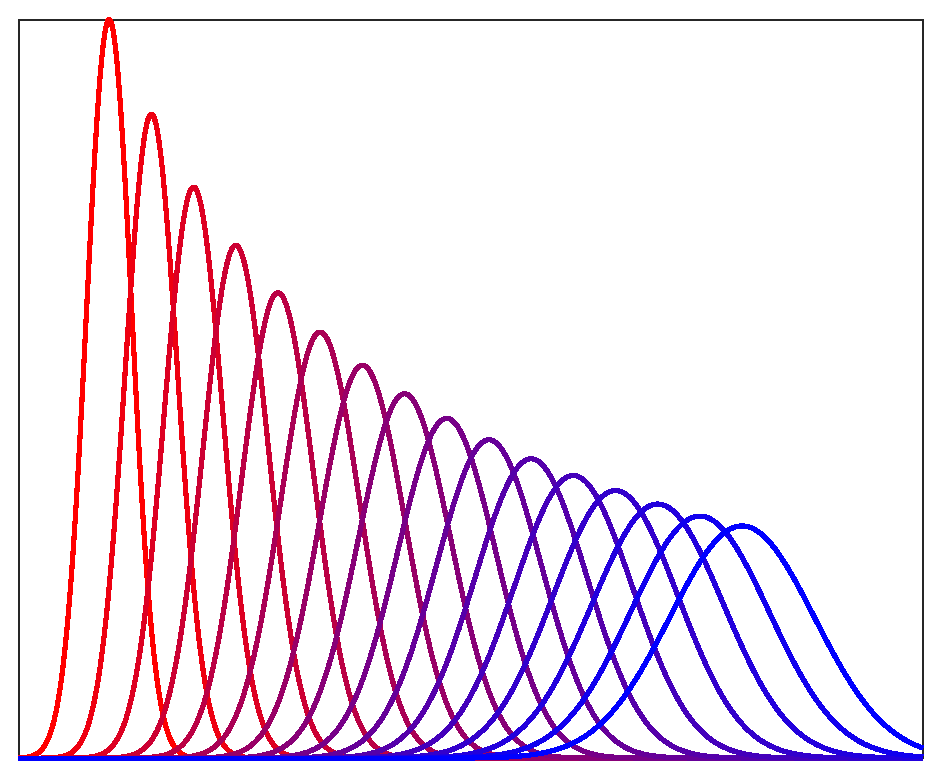
\includegraphics[width=.25\linewidth]{gaussian-1d/interp-density}&
\includegraphics[width=.2\linewidth]{gaussian-1d/gaussian-param}
\end{tabular}
\caption{\label{fig-1d-gaussian}
Computation of displacement interpolation between two 1-D Gaussians. 
%
Denoting $\Gg_{m,\si}(x) \eqdef \frac{1}{\sqrt{2\pi}s}e^{-\frac{(x-m)^2}{2s^2}}$ the Gaussian density, it thus shows 
the interpolation $\Gg_{(1-t)m_0+t m_1,(1-t)\si_0+t \si_1}$.
}
\end{figure}






% !TEX root = ../CourseOT.tex

%%%%%%%%%%%%%%%%%%%%%%%%%%%%%%%%%%%%%%%%%%%%%%%%%%%%%%%%%%%%%%%%%%%%%%%%%%%
%%%%%%%%%%%%%%%%%%%%%%%%%%%%%%%%%%%%%%%%%%%%%%%%%%%%%%%%%%%%%%%%%%%%%%%%%%%
%%%%%%%%%%%%%%%%%%%%%%%%%%%%%%%%%%%%%%%%%%%%%%%%%%%%%%%%%%%%%%%%%%%%%%%%%%%
\section{Kantorovitch Relaxation}

%%%%%%%%%%%%%%%%%%%%%%%%%%%%%%%%%%%%%%%%%%%%%%%%%%%%%%%%%%%%%%%%%%%%%%%%%%%
\subsection{Discrete Relaxation}

Monge discrete matching problem is problematic because it cannot be applied when $n \neq m$. One needs to take into account masses $(\a_i,\b_j)$ to handle this more general situation. 
%
Monge continuous formulation~\eqref{eq-monge-continuous} using push-forward is also problematic because it can be the case that there is no transport map $T$ such that $T_\sharp \al = \be$, for instance when $\al$ is made of a single Dirac to be mapped to several Dirac. Associated to this, it is not symmetric with respect to exchange of $\al$ and $\be$ (one can map two Diracs to a single one, but not the other way).
%
Also, these are non-convex optimization problem which are not simple to solve numerically. 
 
The key idea of~\cite{Kantorovich42} is to relax the deterministic nature of transportation, namely the fact that a source point $x_i$ can only be assigned to another, or transported to one and one location $T(x_i)$ only. Kantorovich proposes instead that the mass at any point $x_i$ be potentially dispatched across several locations. Kantorovich moves away from the idea that mass transportation should be ``deterministic'' to consider instead a ``probabilistic'' (or ``fuzzy'') transportation, which allows what is commonly known now as ``mass splitting'' from a source towards several targets. This flexibility is encoded using, in place of a permutation $\sigma$ or a map $T$, a coupling matrix $\P  \in \RR_+^{n \times m}$, where $\P_{i,j}$ describes the amount of mass flowing from bin $i$ (or point $x_i$) towards bin $j$ (or point $x_j$), 
$x_i$ towards $y_j$ in the formalism of discrete measures $\al=\sum_i \a_i \de_{x_i}$, $\be=\sum_j \b_j \de_{y_j}$. Admissible couplings are only constrained to satisfy the conservation of mass
\eql{\label{eq-discr-couplings}
	\CouplingsD(\a,\b) \eqdef \enscond{ \P \in \RR_+^{n \times m} }{
		\P \ones_m = \a \qandq 
		\transp{\P} \ones_n = \b	
	},
}
where we used the following matrix-vector notation
\eq{
	\P \ones_m = \left(\sum_j \P_{i,j}\right)_i \in \RR^n
	\qandq
	\transp{\P} \ones_n = \left(\sum_i \P_{i,j}\right)_j \in \RR^m. 
}
The set of matrices $\CouplingsD(\a,\b)$ is bounded, defined by $n+m$ equality constraints, and therefore a convex polytope (the convex hull of a finite set of matrices).

%
Additionally, whereas the Monge formulatio is intrinsically asymmetric, Kantorovich's relaxed formulation is always symmetric, in the sense that a coupling $\P$ is in  $\CouplingsD(\a,\b)$ if and only if  $\transp{\P}$ is in $\CouplingsD(\b,\a)$.

Kantorovich's optimal transport problem now reads
\eql{\label{eq-kanto-discr} 
	\MKD_{\C}(\a,\b) \eqdef 
	\umin{\P \in \CouplingsD(\a,\b)}
		\dotp{\C}{\P} \eqdef \sum_{i,j} \C_{i,j} \P_{i,j}. 
}
This is a linear program, and as is usually the case with such programs, its solutions are not necessarily unique. 



%%%%%%%%%%
\paragraph{Linear programming algorithms.}

The reference algorithms to solve~\eqref{eq-mk-discr} are network simplexes. There exists instances of this method which scale like  $O(n^3 \log n)$. Alternative include interior points, which are usually inferior on this particular type of linear program.

%%%%%%%%%%
\paragraph{1-D cases.}

In 1-D, if $c(x,y)=|x-y|^p$ on $\Xx=\Yy=\RR$ with $p \geq 1$, then an optimal transport map is given by an increasing map. So as explained in~\eqref{sec-monge-pbm}, the case $n=m$ and $\a_i=\b_j=\frac{1}{n}$ is solved in $O(n \log(n))$ operations. 
%
In the general case, an optimal coupling matrix $\P$ can be computed similarly in $O(n\log(n)+m\log(m))$ by sorting the points and then sweeping the mass in a single pass from left to right \todo{explain more}.


%%%%%%%%%%
\paragraph{Permutation Matrices as Couplings} 

We restrict our attention to the special case $n=m$ and $\a_i=\b_i=1$ (up to a scaling by $1/n$, these are thus probability measures).
%
In this case one can solve Monge optimal matching problem~\eqref{eq-optimal-assignment}, and it is convenient to re-write it using permutation matrices. 
%
For a permutation $\si\in\Perm(n)$, we write $\P_{\si}$ for the corresponding permutation matrix,
\eql{\label{eq-perm-matrices}
		\foralls (i,j) \in \range{n}^2, \quad
		(\P_{\si})_{i,j} = \choice{
			1 \qifq j=\si_i, \\
			0 \quad\text{otherwise.} 
		}
} 
We denote the set of permutation matrices as
\eq{
	\Pp_n \eqdef \enscond{\P_\si}{ \si\in\Perm(n) }, 
}
which is a discrete, hence non-convex, set. One has
\eq{
	\dotp{\C}{\P_{\si}} = \sum_{i=1}^n \C_{i,\si_i}
}
so that~\eqref{eq-optimal-assignment} is equivalent to the non-convex optimization problem
\eq{
	\umin{\P \in \Pp_n} \dotp{\C}{\P}. 
}

In contrast, one has that $\CouplingsD(\a,\b) = \Bb_n$ is equal to the convex set of bistochastic matrices 
\eq{
	\Bb_n \eqdef \enscond{ \P \in \RR_+^{n \times n} }{\P \ones_n = \P^\top \ones_n = \ones_n}
}
so that Kantorovitch problem reads 
\eq{
	\umin{\P \in \Bb_n} \dotp{\C}{\P}. 
}
The set of permutation matrices is strictly included in the set of bistochastic matrices, and more precisely
\eq{
	\Pp_n = \Bb_n \cap \{0,1\}^{n \times n}.
}
This shows that one has the following obvious relation between the cost of Monge and Kantorovitch problem
\eq{
	\umin{\P \in \Bb_n} \dotp{\C}{\P} \leq \umin{\P \in \Pp_n} \dotp{\C}{\P}. 
}
We will now show that there is in fact an equality between these two costs, so that both problems are in some sense equivalent. 


For this, we will make a detour through more general linear optimization problem of the form $\umin{\P \in \Cc} \dotp{\C}{\P}$ for some compact convex set $\Cc$. We firs introduce the notion of extremal point, which are intuitively the vertices of $\Cc$
\eq{
	\text{Extr}(\Cc) \eqdef \enscond{\P}{ \foralls (Q,R) \in \Cc^2, \P = \frac{Q+R}{2} \Rightarrow Q=R }.
}
So to show that $\P \notin \text{Extr}(\Cc)$ is suffices to split $\P$ as $\P = \frac{Q+R}{2}$ with $Q \neq R$ and $(Q,R) \in \Cc^2$.
%
We will assume the following fundamental result.

\begin{prop}
	If $\Cc$ is compact, then $\text{\upshape Extr}(\Cc) \neq 0$.
\end{prop}

The fact that $\Cc$ is compact is crucial, for instance the set $\enscond{(x,y) \in \RR_+^2}{ xy \geq 1}$ has no extremal point. 

We can now use this result to show the following fundamental result, namely that there is always a solution to a linear program which is an extremal point.
% 
Note that of course the set of solution (which is non-empty because one minimizes a continuous function on a compact) might not be a singleton. 


\begin{figure}
\centering
\begin{tabular}{@{}c@{\hspace{5mm}}c@{}}
\includegraphics[width=.45\linewidth]{birkhoff/extremal-pts}&
\includegraphics[width=.45\linewidth]{birkhoff/min-cvx}
\end{tabular}
\caption{\label{fig-extremal}
%
Left: extremal points of a convex set. 
Right: the solution of a convex program is a convex set. 
}
\end{figure}


\begin{prop}\label{prop-extr-optim}
	If $\Cc$ is compact, then 
	\eq{
		\text{Extr}(\Cc) \cap \pa{ \uargmin{\P \in \Cc} \dotp{\C}{\P}  } \neq \emptyset.
	}
\end{prop}
\begin{proof}
	One consider $\Ss \eqdef \uargmin{\P \in \Cc} \dotp{\C}{\P}$. 
	%	
	We first note that $\Ss$ is convex (as always for an argmin) and compact, because $\Cc$ is compact and the objective function is continuous, so that $\text{Extr}(\Ss) \neq \emptyset$.
	%
	We will show that $\text{Extr}(\Ss) \subset \text{Extr}(\Cc)$. 
	\todo{finish}
\end{proof}

The following theorem states that the extremal points of bistochastic matrices are the permutation matrices. It implies as a corollary that the cost of Monge and Kantorovitch are the same, and that they share a common solution. 


\begin{thm}[Birkhoff and von Neumann]\label{thm-birkh-vnm}
	One has $\text{Extr}(\Bb_n) = \Pp_n$.
\end{thm}
\begin{proof}
	We first show the simplest inclusion $\Pp_n \subset \text{Extr}(\Bb_n)$. Indeed it follows from the fact that $\text{Extr}([0,1]) = \{0,1\}$. Take $\P \in \Pp_n$, if $\P=(Q+R)/2$ with $Q_{i,j},R_{i,j} \in [0,1]$, since $\P_{i,j} \in \{0,1\}$ then necessarily $Q_{i,j}=R_{i,j} \in \{0,1\}$.
	
	Now we show $\text{Extr}(\Bb_n) \subset \Pp_n$ by showing that $\Pp_n^c \subset \text{Extr}(\Bb_n)^c$ where the complementary are computed inside the larger set $\Bb_n$. So picking $\P \in \Bb_n \backslash \Pp_n$, we need to split $\P = (Q+R)/2$ where $Q,R$ are distinct bistochastic matrices. 
	%
	As shown on figure~\ref{fig-extremal}, $\P$ defines a partite graph linking two sets of $n$ vertices. 
	%
	This graph is composed of isolated edge when $\P_{i,j}=1$ and connected edges corresponding to $0 < \P_{i,j} <1$.
	If $i$ is such a connected vertex on the left (similarly for $j$ on the right), because $\sum_j \P_{i,j}=1$, there is necessarily at least two edges $(i,j_1)$ and $(i,j_2)$ emating from it (similarely on the right there are at least two converging edges $(i_1,j)$ and $(i_2,j)$). This means that by following these connexions, one necessarily can extract a cycle (if not, one could alway extend it by the previous remarks) of the form
	\eq{
		(i_1,j_1,i_2,j_2,\ldots,i_p,j_p), 
		\quad \text{i.e.}\quad i_{p+1}=i_1.
	}
	We assume this cycle is the shortest one among all this (finite) ensemble of cycle. Along this cycle, the left-right and right-left edges satisfy
	\eq{
		0 < \P_{i_s,j_s}, \P_{j_s,i_{s+1}} < 1.
	}
	The $(i_s)_s$ and $(j_s)_s$ are also all distincts because the cycle is the shortest. Lets pick
	\eq{
		\epsilon \eqdef \umin{0 \leq s \leq p} \{ \P_{i_s,j_s}, \P_{j_s,i_{s+1}}, 1-\P_{i_s,j_s}, 1-P_{j_s,i_{s+1}} \}
	}
	so that $0 < \epsilon < 1$. As shown on Figure~\ref{fig-extremal}, right, we split the graph in two set of edges, left-right and right-left
	\eq{
		\Aa \eqdef \{(i_s,j_s)\}_{s=1}^p
		\qandq 
		\Bb \eqdef \{(j_s,i_{s+1})\}_{s=1}^p.
	}
	We define then two matrices as
	\eq{
		Q_{i,j} \eqdef 
		\choice{
			\P_{i,j} \qifq (i,j) \notin \Aa \cup \Bb, \\
			\P_{i,j}+\epsilon/2 \qifq (i,j) \in \Aa, \\
			\P_{i,j}-\epsilon/2 \qifq (i,j) \in \Bb, 		
		}
		\qandq
		R_{i,j} \eqdef 
		\choice{
			\P_{i,j} \qifq (i,j) \notin \Aa \cup \Bb, \\
			\P_{i,j}-\epsilon/2 \qifq (i,j) \in \Aa, \\
			\P_{i,j}+\epsilon/2 \qifq (i,j) \in \Bb, 		
		}.
	}
	Because of the choice of $\epsilon$, one has $0 \leq Q_{i,j}, R_{i,j} \leq 1$.
	Because each left-right edge in $\Aa$ is associated to a right-left edge in $\Bb$, (and the other way) the
	sum constraint on the row (and on the column) is maintain, so that $U,V \in \Bb_n$. Finally, note that $\P=(P+Q)/2$.	
\end{proof}



\begin{figure}
\centering
\begin{tabular}{@{}c@{\hspace{5mm}}c@{}}
\includegraphics[width=.7\linewidth]{birkhoff/bipartite}&
\includegraphics[width=.25\linewidth]{birkhoff/bipartite-split}
\end{tabular}
\caption{\label{fig-extremal}
%%
Left: the support of the coupling $\P$ defines a bipartite graph.
Right: splitting of this graph in two set of edges.
}
\end{figure}

By putting together Proposition~\ref{prop-extr-optim} and Theorem~\ref{thm-birkh-vnm}, one obtains that for the discrete optimal problem with empirical measures, Monge and Kantoritch problems are equivalent.

\begin{cor}[Kantorovich for matching]\label{prop-matching-kanto}
	If $m=n$ and $\a=\b=\ones_n$, then there exists an optimal solution for Problem~\eqref{eq-mk-discr} $\P_{\si^\star}$, which is a permutation matrix associated to an optimal permutation $\si^\star \in \Perm(n)$ for Problem~\eqref{eq-optimal-assignment}.	
\end{cor}

The following proposition shows that these problems result in fact in the same optimum, namely that one can always find a permutation matrix that minimizes Kantorovich's problem~\eqref{eq-mk-discr} between two uniform measures $\a=\b=\ones_n/n$, which shows that the Kantorovich relaxation is \emph{tight} when considered on assignment problems. %Note however that some computational algorithm, which are combinatorial in nature, are dedicated to the case of uniform histograms with the same number of points (see Chapter~\ref{c-algo-basics}). 
%
% Figure~\ref{fig-matching-kantorovitch} shows on the left a 2-D example of optimal matching corresponding to this special case. 

%\begin{figure}
%\centering
%\begin{tabular}{@{}c@{\hspace{5mm}}c@{}}
%\includegraphics[width=.25\linewidth]{matching-kantorovitch/matching}&
%\includegraphics[width=.25\linewidth]{matching-kantorovitch/weighted}
%\end{tabular}
%\caption{\label{fig-matching-kantorovitch}
%%
%Comparison of optimal matching and generic couplings. A black segment between $x_i$ and $y_j$ indicates a non-zero element in the displayed optimal coupling $\P_{i,j}$ solving~\eqref{eq-mk-discr}.
%%
%Left: optimal matching, corresponding to the setting of Proposition~\eqref{prop-matching-kanto} (empirical measures with the same number $n=m$ of points).
%%
%Right: these two weighted point clouds cannot be matched; instead a Kantorovich coupling can be used to associate two arbitrary discrete measures.  
%}
%\end{figure}


\begin{rem}[General case] For general input measure, one does not have equivalence between Monge and Kantorovitch problems (since the Monge constraint is in general empty). But the support of the optimal coupling $\P$ still enjoys some strong regularity, in particular, it defines a cycle-free bipartite graph. This implies in particular that the resulting $\P$ matrix is sparse, for instance one can show that there are always solutions with less than $n+m-1$ non-zero elements.	
\end{rem}

%%%%%%%%%%%%%%%%%%%%%%%%%%%%%%%%%%%%%%%%%%%%%%%%%%%%%%%%%%%%%%%%%%%%%%%%%%%
\subsection{Relaxation for Arbitrary Measures}

%%%
\paragraph{Continuous couplings.}

The definition of $\MK_\c$ in~\eqref{eq-kanto-discr} is extended to arbitrary measures by considering couplings $\pi \in \Mm_+^1(\X \times \Y)$ which are joint distributions over the product space. 
%
The marginal constraint $\P\ones_m=\a, \P\ones_n=\b$ must be replaced by ``integrated'' versions, which are written $\pi_1 = \al$ and $\pi_2 = \be$, where $(\pi_1,\pi_2) \in \Mm(\Xx) \times \Mm(\Yy)$ are the two marginals. 
%
They are defined as $\pi_1 \eqdef P_{1\sharp} \pi$ and $\pi_2 \eqdef P_{2\sharp} \pi$ the two marginals of $\pi$, which are defined using push-forward by the projectors $P_1(x,y)=x$ and $P_2(x,y)=y$.

A heuristic way to understand the marginal constraint $\pi_1 = \al$ and $\pi_2 = \be$, which mimics the discrete case where one sums along the rows and columns is to write
\eq{
	\int_\Yy \d\pi(x,y) = \d\al(x)
	\qandq
	\int_\Xx \d\pi(x,y) = \d\be(y),
}
and the mathematically rigorous way to write this, which corresponds to the change of variables formula, is 
\eq{
	\foralls (f,g) \in \Cc(\Xx) \times \Cc(\Yy), \quad
	\int_{\Xx \times \Yy} f(x) \d\pi(x,y) = \int_\Xx f \d\al
	\qandq
	\int_{\Xx \times \Yy} \d\pi(x,y) = \int_\Yy g \d\be.
}	
%
Using~\eqref{eq-equiv-pushfwd}, these marginal constraints are also equivalent to imposing that $\pi(A \times \Y)=\al(A)$ and $\pi(\X \times B)=\be(B)$ for sets $A \subset \X$ and $B \subset \Y$.

Replacing continuous functions by indicator function, one can also rephrase this conservation of mass constraint as
\eq{
	\foralls (A,B) \in \X \times \Y, \quad
		\pi(A \times \Y) = \al(A)
		\qandq
		\pi(\X \times B) = \be(B). 
}

In the general case, the mass conservation constraint~\eqref{eq-discr-couplings} should thus rewritten as a marginal constraint on joint probability distributions
\eql{\label{eq-coupling-generic}
	\Couplings(\al,\be) \eqdef 
	\enscond{
		\pi \in \Mm_+^1(\X \times \Y)
	}{
		\pi_1 = \al
		\qandq
		\pi_2 = \be
	}.
} 

The discrete case, when $\al=\sum_i \a_i \de_{x_i}$, $\be=\sum_j \a_j \de_{x_j}$, the constraint $\pi_1=\al$ and $\pi_2=\be$ necessarily imposes that $\pi$ is discrete, supported on the set $\{(x_i,y_j)\}_{i,j}$, and thus has the form $\pi = \sum_{i,j} \P_{i,j} \de_{(x_i,y_j)}$. The discrete formulation is thus a special case (and not some sort of approximation) of the continuous formulation. 

The set $\Couplings(\al,\be)$ is always non-empty because it contains at least the tensor product coupling $\al \otimes \be$ defined by $\d(\al\otimes\be)(x,y)=\d\al(x)\d\be(y)$ i.e.
\eq{
	\foralls h \in \Cc(\Xx\times\Yy), \quad
	\int_{\X \times \Y} h(x,y)\d(\al\otimes\be)(x,y) = \int_\X (\int_\Y h(x,y) \d\be(y)) \d\al(x)
	=  \int_\X (\int_\Y h(x,y) \d\al(x) ) \d\be(y).
} 
Indeed, $(\al\otimes\be)_1 = \al$ since
\eq{
	\foralls f \in \Cc(\X), \quad
	\int_\X f(x) \d (\al\otimes\be)_1(x)
	= 
	\int_{\X \times \Y} f(x) d\al(x)\d\be(y)
	= \int_\X f(x) \d\al(x) \int_\Y \d\be
	= \int_\X f(x) \d\al(x)
}
because $\int_\Y \d\be=1$.

A very different (concentrated) type of coupling is defined when there exists a map $T: \X \rightarrow \Y$ such that $T_\sharp \al = \be$ (i.e. the constraint set of Monge's problem~\eqref{eq-monge-continuous} is non-empty). In this case, one has that $\pi = (\Id,T)_\sharp \al \in \Couplings(\al,\be)$. This coupling is defined though the integrated definition of push-forward as
\eq{
	\foralls h \in \Cc(\Xx\times\Yy), \quad
	\int_{\X \times \Y} h(x,y)\d\pi(x,y)
	= 
	\int_{\X} h(x,T(x))\d\al. 
} 
In particular, applying this formula to $h(x,y)=f(x)$ or $h(x,y)=g(y)$  shows that $\pi_1=\al$ and $\pi_2=\be$.



%
%
%\begin{figure}
%\centering
%\begin{tabular}{@{}c@{\hspace{5mm}}c@{\hspace{5mm}}c@{}}
%\includegraphics[width=.22\linewidth]{settings/discrete}&
%\includegraphics[width=.22\linewidth]{settings/semi-discrete}&
%\includegraphics[width=.22\linewidth]{settings/continuous}\\
%Discrete & Semi-discrete & Continuous
%\end{tabular}
%\caption{\label{fig-settings}
%Schematic viewed of input measures $(\al,\be)$ and couplings $\Couplings(\al,\be)$ encountered in the three main scenario for Kantorovich OT. Chapter~\ref{c-algo-semidiscr} is dedicated to the semi-discrete setup.
%}
%\end{figure}


%%%
\paragraph{Continuous Kantorovitch problem.}


The Kantorovich problem~\eqref{eq-kanto-discr} is then generalized as 
\eql{\label{eq-mk-generic}
	\MK_\c(\al,\be) \eqdef 
	\umin{\pi \in \Couplings(\al,\be)}
		\int_{\X \times \Y} \c(x,y) \d\pi(x,y).
}
This is an infinite-dimensional linear program over a space of measures. 


% Figure~\ref{fig-couplings} shows examples of discrete and continuous optimal coupling solving~\eqref{eq-mk-generic}.
% Figure~\ref{fig-couplings-simple} shows other examples of optimal 1-D couplings, involving discrete and continuous marginals.

%\begin{figure}
%\centering
%\begin{tabular}{@{}c@{\hspace{10mm}}c@{}}
%\includegraphics[width=.2\linewidth]{couplings/couplings-continuous}&
%\includegraphics[width=.2\linewidth]{couplings/couplings-discr}
%\end{tabular}
%\caption{\label{fig-couplings}
%Left: ``continuous'' coupling $\pi$ solving~\eqref{eq-coupling-generic} between two 1-D measure with density. The coupling is localized along the graph of the Monge map $(x,\T(x))$ (displayed in black).  
%%
%Right: ``discrete'' coupling $\T$ solving~\eqref{eq-mk-discr} between two discrete measures of the form~\eqref{eq-pair-discr}. The non-zero entries $\T_{i,j}$  are display with a black disk at position $(i,j)$ with radius proportional to $\T_{i,j}$.
%}
%\end{figure}


%\begin{figure}
%\centering
%\begin{tabular}{@{}c@{}c@{}c@{}c@{}}
%\includegraphics[width=.2\linewidth]{couplings/couplings-1}&
%\includegraphics[width=.2\linewidth]{couplings/couplings-2}&
%\includegraphics[width=.2\linewidth]{couplings/couplings-3}&
%\includegraphics[width=.2\linewidth]{couplings/couplings-4}
%\end{tabular}
%\caption{\label{fig-couplings-simple}
%Four simple examples of optimal couplings between 1-D distributions, represented as maps above (arrows) and couplings below. Inspired by~\cite{Levy2017review}.
%}
%\end{figure}


On compact domain $(\Xx,\Yy)$, \eqref{eq-mk-generic} always has a solution, because using the weak-* topology (so called weak topology of measures), the set of measure is compact, and a linear function with a continuous $c(x,y)$ is weak-* continuous. And the set of constraint is non empty, taking $\al \otimes \be$. On non compact domain, one needs to impose moment condition on $\al$ and $\be$.

%%%%
\paragraph{Probabilistic interpretation.}

If we denote $X \sim \al$ the fact that the law of a random vector $X$ is the probability distribution $\al$, then the marginal constraint appearing in~\eqref{eq-mk-generic} is simply that $\pi$ is the law of a couple $(X,Y)$ and that its coordinates $X$ and $Y$ have laws $\al$ and $\be$. The coupling $\pi$ encodes the statistical dependency between $X$ and $Y$. For instance, $\pi = \al\otimes \be$ means that $X$ and $Y$ are independent, and it unlikely that such a coupling is optimal. Indeed as stated by Brenier's theorem, optimal coupling for a square Euclidean loss on contrary describe totally dependent variable, which corresponds to a coupling of the form $\pi=(\Id,T)_\sharp \al$ in which case $Y=T(X)$ where $T: \X \rightarrow \Y$ is a measurable map. 

With this remark, problem~\eqref{eq-mk-generic} reads equivalently 
\eql{\label{eq-mk-proba}
	\MK_\c(\al,\be) = 
	\umin{X \times \al, Y \sim \be} \EE(c(X,Y)).
}

%%%%
\paragraph{Monge-Kantorovitch equivalence.}

The proof of Brenier theorem~\ref{thm-brenier}  (detailed in Section~\ref{sec-c-transfo}, Remark~\ref{rem-proof-brenier}) to prove the existence of a Monge map actually studies Kantorovitch relaxation (and makes use of duality), and proves that this relaxation is tight in the sense that it has the same cost as Monge problem. 

Indeed, it shows that the support of an optimal $\pi$ is contained in the subdifferential $\partial \phi$ of a convex function $\phi$, which in general is a set-valued mapping \todo{give the example of a segment split into two equally spaced segments}.
%
When $\alpha$ does not have a density, then $\phi$ is non-smooth and non-smooth points where $\al(\{x\})>0$ leads to mass splitting, for instance moving $\de_{0}$ to $(\de_{-1}+\de{+1})/2$ can be achieved using $\phi(x)=|x|$.  


If $\al$ has a density, then this $\phi$ is differentiable $\al$-almost everywhere and we denote $\T=\nabla\phi$ the unique optimal transport (which is a valid definition almost everywhere and one can use any value at point of non differentiability), then the coupling 
\eq{
	\pi = (\Id,\T)_\sharp \al
	\quad\text{i.e.}\quad
	\foralls h \in \Cc(\Xx \times \Yy), \quad
	\int_{\Xx \times \Yy} h \d \pi = \int_{\Xx} h(x,\T(x)) \d\al(x)
}
is optimal.
In term of random vector, denoting $(X,Y)$ a random vector with law $\pi$, it means that any such optimal random vector satisfies $Y=\T(X)$ where $X \sim \al$ (and of course $\T(X) \sim \be$ by the marginal constraint). 


This key result is similar to Birkoff-von-Neumann Theorem~\ref{prop-matching-kanto} in the sense that it provides conditions ensuring the equivalence between Monge and Kantorovitch problems (note however that Birkoff-von-Neumann does not implies uniqueness). Note however that the settings are radically difference (one is fully discrete while the other requires the sources to  be ``continuous'', i.e. to have a density).


%%%%%%%%%%%%%%%%%%%%%%%%%%%%%%%%%%%%%%%%%%%%%%%%%%%%%%%%%%%%%%%%%%%%%%%%%%%
\subsection{Metric Properties}

%%%%
\paragraph{OT defines a distance.}

An important feature of OT is that it defines a distance between histograms and probability measures as soon as the cost matrix satisfies certain suitable properties. Indeed, OT can be understood as a canonical way to lift a ground distance between points to a distance between histogram or measures. 

% We first consider the case where, using a term first introduce by~\cite{RubTomGui00}, the ``ground metric'' matrix $\C$ is fixed, representing substitution costs between bins, and shared across several histograms we would like to compare. The following proposition states that OT provides a meaningful distance between histograms supported on these bins.

\begin{prop}\label{prop-metric-histo}
We suppose $n=m$, and that for some $p \geq 1$, $\C=\distD^p=(\distD_{i,j}^p)_{i,j} \in \RR^{n \times n}$ where $\distD \in \RR_+^{n \times n}$ is a distance on $\range{n}$, \emph{i.e.}
\begin{enumerate}% [label=(\roman*)]
	\item $\distD \in \RR_+^{n \times n}$ is symmetric; 
	\item $\distD_{i,j}=0$ if and only if $i=j$; 
	\item $\foralls (i,j,k) \in \range{n}^3, \distD_{i,k} \leq \distD_{i,j}+\distD_{j,k}$.
\end{enumerate}
Then 
\eql{\label{eq-wass-p-disc}
	\WassD_p(\a,\b) \eqdef \MKD_{\distD^p}(\a,\b)^{1/p}
}
(note that $\WassD_p$ depends on $\distD$) defines the $p$-Wasserstein distance on $\Si_n$, \emph{i.e.} $\WassD_p$ is symmetric, positive, $\WassD_p(\a,\b)=0$ if and only if $\a = \b$, and it satisfies the triangle inequality
\eq{
	\foralls \a,\a',\b \in \Si_n, \quad \WassD_p(\a,\b) \leq \WassD_p(\a,\a') + \WassD_p(\a',\b).
}
\end{prop}

\begin{proof}
Symmetry and definiteness of the distance are easy to prove: since $\C = \distD^p$ has a null diagonal, $\WassD_p(\a,\a)=0$, with corresponding optimal transport matrix $\P^\star=\diag(\a)$; by the positivity of all off-diagonal elements of $\distD^p$, $\WassD_p(\a,\b)>0$ whenever $\a\ne \b$ (because in this case, an admissible coupling necessarily has a non-zero element outside the diagonal); by symmetry of $\distD^p$, $\WassD_p(\a,\b)=0$ is itself a symmetric function. 


To prove the triangle inequality of Wasserstein distances for arbitrary measures, \cite[Theorem 7.3]{Villani03} uses the gluing lemma, which stresses the existence of couplings with a prescribed structure. 
% Closed forms for such couplings exist in the discrete case which we can readily use. 
In the discrete setting, the explicit constuction of this glued coupling is simple.
%
Let $\a,\b,\VectMode{c} \in\simplex_n$. Let $\P$ and $\Q$ be two optimal solutions of the transport problems between $\a$ and $\b$, and $\b$ and $\VectMode{c}$ respectively. 
%
We define $\bar\b_j \eqdef \b_j$ if $\b_j>0$ and set otherwise $\bar\b_j=1$ (or actually any other value). We then define 
\eq{
	\SS \eqdef \P \diag(1/\bar\b) \Q \in \RR_+^{n \times n}.
} 
We remark that $\SS \in \U(\a,\VectMode{c})$ because 
\eq{
	\SS \ones_n  = \P \diag(1/\bar\b) \Q \ones_n = \P (\b / \bar\b) = \P \ones_{\Supp(\b)} = \a
}
where we denoted $\ones_{\Supp(\b)}$ the indicator of the support of $\b$, and we use the fact that $\P \ones_{\Supp(\b)} = \P \ones = \b$ because necessarily $\P_{i,j} = 0$ for $j \notin \Supp(\b)$.
Similarly one verifies that $\SS^\top \ones_n = \VectMode{c}$.


The triangle inequality follows from
%   notice that $\SS_{i\cdot k}$ being therefore a matrix of $\U(\a,\b)$ we can write:
$$\begin{aligned}
\WassD_p(\a,\VectMode{c})&=\left(\min_{\P\in U(\a,\VectMode{c})}\dotp{\P}{\distD^p}\right)^{1/p} \leq \dotp{\SS}{\distD^p}^{1/p}\\
&= \left(\sum_{ik} \distD^p_{ik}\sum_{j} \frac{\P_{ij}\Q_{jk}}{\bar\b_j}\right)^{1/p} \leq \left(\sum_{ijk} \left(\distD_{ij}+\distD_{jk}\right)^p \frac{\P_{ij}\Q_{jk}}{\bar\b_j}\right)^{1/p} \\
& \leq \left(\sum_{ijk} \distD^p_{ij} \frac{\P_{ij}\Q_{jk}}{\bar\b_j}\right)^{1/p} + \left(\sum_{ijk}\distD^p_{jk} \frac{\P_{ij}\Q_{jk}}{\bar\b_j}\right)^{1/p} \\
&= \left(\sum_{ij} \distD^p_{ij}\P_{ij} \sum_k \frac{\Q_{jk}}{\bar\b_j}\right)^{1/p} + \left(\sum_{jk} \distD^p_{jk} \Q_{jk} \sum_i \frac{\P_{ij}}{\bar\b_j}\right)^{1/p}\\
&= \left(\sum_{ij} \distD^p_{ij}\P_{ij}\right)^{1/p} + \left(\sum_{jk} \distD^p_{jk} \Q_{jk}\right)^{1/p}\\ 
&= \WassD_p(\a,\b) +\WassD_p(\b,\b).
\end{aligned}
$$
%
The first inequality is due to the suboptimality of $\SS$, the second is the usual triangle inequality for elements in $\distD$, and the third comes from Minkowski's inequality.
\end{proof}

Proposition~\ref{prop-metric-histo} generalizes from histogram to arbitrary measures that need not be discrete.

\begin{prop}\label{prop-metric-measure}
We assume $\X=\Y$, and that for some $p \geq 1$, $\c(x,y)=\dist(x,y)^p$ where $\dist$ is a distance on $\X$, \emph{i.e.} \\
	\hbox{}\qquad (i) $\dist(x,y) = \dist(y,x) \geq 0$;  \\
	\hbox{}\qquad (ii)  $\dist(x,y)=0$ if and only if $x=y$;  \\
	\hbox{}\qquad (ii)  $\foralls (x,y,z) \in \X^3, \dist(x,z) \leq \dist(x,y)+\dist(y,z)$. \\
Then 
\eql{\label{eq-defn-wass-dist}
	\Wass_p(\al,\be) \eqdef \MK_{\dist^p}(\al,\be)^{1/p}
}
(note that $\Wass_p$ depends on $\dist$) defines the $p$-Wasserstein distance on $\X$, \emph{i.e.} $\Wass_p$ is symmetric, positive, $\Wass_p(\al,\be)=0$ if and only if $\al = \be$, and it satisfies the triangle inequality
\eq{
	\foralls (\al,\be,\ga) \in  \Mm_+^1(\X)^3, \quad \Wass_p(\al,\ga) \leq \Wass_p(\al,\be) + \Wass_p(\be,\ga).
}
\end{prop}

This distance $\Wass_p$ defined though Kantorovitch problem~\eqref{eq-defn-wass-dist} should be contrasted with the distance $\tilde\Wass$ obtained using Monge's problem~\eqref{eq-monge-distance}. Kantorovitch distance is always finite, while Monge's one might be infinite if the constraint set $\enscond{T}{T_\sharp \al=\be}$ is empty. In fact, one can show that as soon as this constraint set is non-empty, and even if no optimal $T$ exists, then one has $\Wass_p = \tilde\Wass_p$, which is a non-trivial result. Kantorovitch distance should thus be seen as a (convex) relaxation of Monge's distance, which behave in a much nicer way, as we will explore next (it is continuous with respect to the convergence in law topology.


%%%%
\paragraph{Convergence in law topology.}

Let us first note that on a compact space, all $W_p$ distance defines the same topology (although they are not equivalent, the notion of converging sequence is the same).

\begin{prop}\label{prop-comp-wass-p}
	On a compact space $\Xx$, one has for $p \leq q$
	\eq{
		W_p( \al,\be ) \leq W_q(\al,\be) \leq \text{\upshape diam}(\Xx)^{\frac{q-p}{q}} W_p(\al,\be)^{\frac{q}{p}}
	}
\end{prop}
\begin{proof}
	The left inequality follows from Jensen inequality, $\phi(\int c(x,y) \d\pi(x,y)) \leq \int \phi(c(x,y)) \d\pi(x,y)$, applied to any probability distribution $\pi$ and to the convex function $\phi(r)=r^{q/p}$ to $c(x,y)=\norm{x-y}^p$, so that one gets
	\eq{
		\pa{\int \norm{x-y}^{p} \d\pi(x,y)}^{\frac{q}{p}} \leq \int \norm{x-y}^{q} \d\pi(x,y).
	} 	
	The right inequality follows from
	\eq{
		\norm{x-y}^q \leq \text{diam}(\Xx)^{q-p} \norm{x-y}^p.
	}
\end{proof}

The Wasserstein distance $\Wass_p$ has many important properties, the most important one being that it is a weak distance, \emph{i.e.} it allows to compare singular distributions (for instance discrete ones) and to quantify spatial shift between the supports of the distributions. This corresponds to the notion of weak$^*$ convergence.

\begin{defn}[Weak$^*$ topology]\label{dfn-weak-conv}
	$(\al_k)_k$ converges weakly$^*$ to $\al$ in $\Mm_+^1(\Xx)$ (denoted $\al_k \rightharpoonup \al$) if and only if for any continuous function $f \in \Cc(\Xx)$, $\int_\Xx f \d\al_k \rightarrow \int_\Xx f \d\al$.
\end{defn}

In term of random vectors, if $X_n \sim \al_n$ and $X \sim \al$ (not necessarily defined on the same probability space), the weak$^*$ convergence corresponds to the convergence in law of $X_n$ toward $X$.

\begin{defn}[Strong topology]
The simplest distance on Radon measures is the total variation norm, which is the dual norm of the $L^\infty$ norm on $\Cc(\Xx)$ and whose topology is often called the ``strong'' topology
\eq{
	\norm{\al-\be}_{TV} \eqdef \usup{\norm{f}_\infty \leq 1} \int f \d(\al-\be)
	 = |\al-\be|(\Xx)
}
where $|\al-\be|(\Xx)$ is the mass of the absolute value of the difference measure. When $\al-\be=\rho \d x$ has a density, then $\norm{\al-\be}_{TV}=\int |\rho(x)| \d x=\norm{\rho}_{L^1(\d x)}$ is the $L^1$ norm associated to $\d x$. When $\al-\be=\sum_i u_i \de_{z_i}$ is discrete, then $\norm{\al-\be}_{TV}=\sum_i |u_i|=\norm{u}_{\ell^1}$ is the discrete $\ell^1$ norm. 
\end{defn}

In the special case of Diracs, having $\int f \d\de_{x_n} = f(x_n) \rightarrow \int f \d\de_{x} = f(x)$ for any continuous $f$ is equivalent to $x_n \rightarrow x$. One can then contrast the strong topology with the Wasserstein distance, if $x_n \neq x$, 
\eq{
	\norm{\de_{x_n}-\de_x}_{TV}=2
	\qandq
	W_p(\de_{x_n},\de_x) = d(x_n,x).
}
This shows that for the strong topology, Diracs never converge, while they do converge for the Wasserstein distance. In fact it is a powerful property of the Wasserstein distance, which is regular with respect to the weak$^*$ topology, and metrizes it.

\begin{prop}
	If $\Xx$ is compact, $\al_k \rightharpoonup \al$ if and only if $W_p(\al_k,\al) \rightarrow 0$. 
\end{prop}

The proof of this proposition requires the use of duality, and is delayed to later, see Proposition~\ref{cor-topol-wass}. 
On non-compact spaces, one needs also to impose the convergence of the moments up to order $p$.
%
Note that there exists alternative distances which also metrize weak convergence. The simplest one are Hilbertian kernel norms, which are detailed in Section~\ref{sec-dual-norms}.

Another example of such a weak convergence is the fact that on $\Xx=\RR$
\eq{
	\frac{1}{n} \sum_{k=1}^n \de_{k/n} \rightharpoonup \Uu_{[0,1]}
}
(convergence toward the uniform measure on $[0,1]$), which comes from the convergence of Riemann sums 
\eq{
	\foralls f \in \Cc(\RR), \quad
	\frac{1}{n} \sum_{k=1}^n f(k/n) \longrightarrow \int_0^1 f(x) \d x.
}
In contrary, one has that for all $n$, since the two measure are mutually singular
\eq{
	\norm{ \frac{1}{n} \sum_{k=1}^n \de_{k/n} - \Uu_{[0,1]}}_{TV} = 
	\norm{ \frac{1}{n} \sum_{k=1}^n \de_{k/n} }_{TV} +  \norm{\Uu_{[0,1]}}_{TV} = 2
}
so that there is no strong convergence. 


 
 
%%%%%
\paragraph{Applications and implications}

Applications for having a geometric distance : barycenters, shape registration loss functions, density fitting
% !TEX root = ../CourseOT.tex


%%%%%%%%%%%%%%%%%%%%%%%%%%%%%%%%%%%%%%%%%%%%%%%%%%%%%%%%%%%%%%%%%%%%%%%%%%%
%%%%%%%%%%%%%%%%%%%%%%%%%%%%%%%%%%%%%%%%%%%%%%%%%%%%%%%%%%%%%%%%%%%%%%%%%%%
%%%%%%%%%%%%%%%%%%%%%%%%%%%%%%%%%%%%%%%%%%%%%%%%%%%%%%%%%%%%%%%%%%%%%%%%%%%
\section{Sinkhorn}

%%%%%%%%%%%%%%%%%%%%%%%%%%%%%%%%%%%%%%%%%%%%%%%%%%%%%%%%%%%%%%%%%%%%%%%%%%%
\subsection{Entropic Regularization for Discrete Measures}


%%%%%
\paragraph{Relative entropy}

The Kullback-Leibler divergence is defined as
\eql{\label{eq-kl-defn}
	\KLD(\P|\Q) \eqdef \sum_{i,j}  \P_{i,j} \log\pa{\frac{\P_{i,j}}{\Q_{i,j}}} - \P_{i,j} + \Q_{i,j}.
}
with the convention $0\log(0)=0$ and $\KLD(\P|\Q)=+\infty$ if there exists some $(i,j)$ such that $\Q_{i,j}=0$ but $\P_{i,j} \neq 0$. 
%
The special case $\KLD(\P|\ones_{n \times m})$ corresponds to minus the Shannon-Boltzmann entropy
\eq{
	\HD( \P ) = -\KLD(\P|\ones_{n \times m}) = -\sum_{i,j} \P_{i,j} \log(\P_{i,j}). 
}
%
The function $\KLD(\cdot|\Q)$ is strongly convex, because its hessian is $\partial^2 \KLD(\P|\Q)=\diag(1/\P_{i,j})$ and $\P_{i,j} \leq 1$. 
%
Note that since in what follows $\P$ and $\Q$ are actually probability distributions, one has 
\eq{
	\KLD(\P|\Q) = \sum_{i,j}  \P_{i,j} \log\pa{\frac{\P_{i,j}}{\Q_{i,j}}},
} 
but considering the extra terms gives cleaner expressions, in particular $\nabla \KLD(\P|\Q) = \log(\P/\Q)$ and duality formula reads more nicely. And for later, it will be important to have this normalization when considering unbalanced OT (see Section~\ref{sec-unbalanced}).

$\KL$ is a particular instance (and actually the unique case) of both a $\phi$-divergence (as defined in Section~\ref{sec-phi-div}) and a Bregman divergence. This unique property is at the heart of the fact that this regularization leads to elegant algorithms and a tractable mathematical analysis. One thus has $\KLD(\P|\Q) \geq 0$ and  $\KLD(\P|\Q)=0$ if and only if $\P=\Q$ (see Proposition~\ref{phi-div-positive}).


%%%%%
\paragraph{Entropic Regularization for Discrete Measures.}

The idea of the entropic regularization of optimal transport is to use $\KLD$ as a regularizing function to obtain approximate solutions to the original transport problem~\eqref{eq-mk-discr}:
\eql{\label{eq-regularized-discr}
	\MKD_\C^\epsilon(\a,\b) \eqdef 
	\umin{\P \in \CouplingsD(\a,\b)}
		\dotp{\P}{\C} + \epsilon \KLD(\P|\a \otimes \b). 
} 
Here we used as a reference measure for the relative entropy $\a \otimes \b = (\a_i \b_j)_{i,j}$.
%
This choice of normalization, specially in this discrete setting, has no importance for the selection of the optimal $\P$ since it only affects the objective by a constant, as shown in the following proposition.

\begin{prop} For $\P \in \CouplingsD(\a,\b)$, one has
\eq{
	\KLD(\P|\a \otimes \b) = 
	\KLD(\P|\a' \otimes \b') - \KLD(\a|\a') - \KL(\b|\b').
} 
\end{prop}

\begin{proof}
This follows from 
\eq{
	\sum_{i,j} \P_{i,j} \log\frac{\P_{i,j}}{\a_i\b_j}
	= 
	\sum_{i,j} \P_{i,j} \log\frac{\P_{i,j}}{\a_i'\b_j'}
	+ 
	\sum_{i,j} \P_{i,j} \pa{\log\frac{\a_i'}{\a_i} + \log\frac{\b_j'}{\b_j}}.
} 
\end{proof}

In the case where $\a_i>0$ and $\b_j>0$ (full support histogram), one could thus replace the reference measure $\a \otimes \b$ by $\ones_{n \times m}$, and thus regularize using the penalty $\HD(\P)$ in place of $\KL(\P|\a \otimes \b)$, resulting in the same solution.
%
The choice of using the reference measure $\a \otimes \b$ is however important to deal with situation where the support of $\a$ and $\b$ can change (so that some coordinate of $\a$ or $\b$ might vanish), and more importantly in the following section which dealds with possibly continuous distributions. Note that it also affect the values of the cost $\MKD_\C^\epsilon(\a,\b)$.


% Figure~\ref{fig-impact-eps} illustrates the effect of the entropy to regularize a linear program over the simples $\simplex_3$ (which can thus be visualized as a triangle in 2-D). Note how the entropy pushes the original LP solution away from the boundary of the triangle. The optimal $\P_\epsilon$ progressively moves toward an ``entropic center'' of the triangle. This is further detailed in the proposition below. The convergence of the solution of that regularized problem towards an optimal solution of the original linear program has been studied by~\cite{CominettiAsympt}.


%\begin{figure}
%\centering
%\includegraphics[width=.5\linewidth]{entropic/simplex}
%\caption{\label{fig-impact-eps}
%Impact of $\epsilon$ on the optimization of a linear function on the simplex, solving $\P_\epsilon = \argmin_{\P \in \simplex_3} \dotp{\C}{\P}-\epsilon\HD(\P)$ for a varying $\epsilon$. 
%}
%\end{figure}


%%%%%
\paragraph{Smoothing effect.}

Since the objective is a $\epsilon$-strongly convex function, problem~\ref{eq-regularized-discr} has a unique optimal solution. 
%
As studied in Section~\ref{}, this smoothing, beyond providing uniqueness, actually leads to $\MKD_\C^\epsilon(\a,\b)$ being a smooth function of $\a, \b$ and $\C$. 
%
The effect of the entropy is to act as a barrier function for the positivity constraint. As we will show next, this forces the solution $\P$ to be strictly positive on the support of $\a \otimes \b$. 

One has the following convergence property.
 
 
\begin{prop}[Convergence with $\epsilon$]\label{prop-convergence-eps}
The unique solution $\P_\epsilon$ of~\eqref{eq-regularized-discr} converges to the optimal solution with maximal entropy within the set of all optimal solutions of the Kantorovich problem, namely
\eql{\label{eq-entropy-conv-1}
	\P_\epsilon \overset{\epsilon \rightarrow 0}{\longrightarrow}
	\uargmin{\P} \enscond{ \KLD(\P|\a \otimes \b) }{
		\P \in \CouplingsD(\a,\b), \dotp{\P}{\C} = \MKD_\C(\a,\b)
	}
}
so that in particular
\eq{
	\MKD_\C^\epsilon(\a,\b) \overset{\epsilon \rightarrow 0}{\longrightarrow} \MKD_\C(\a,\b).
}
One has
\eql{\label{eq-entropy-conv-2}
	\P_\epsilon \overset{\epsilon \rightarrow \infty}{\longrightarrow}
	\a \otimes \b.
}
\end{prop}

\begin{proof}
	\textbf{Case $\epsilon \rightarrow 0$.}
	 We consider a sequence $(\epsilon_\ell)_\ell$ such that $\epsilon_\ell \rightarrow 0$ and $\epsilon_\ell > 0$.	
 	We denote $\P_\ell$ the solution of~\eqref{eq-regularized-discr} for $\epsilon=\epsilon_\ell$. 
	%
	Since $\CouplingsD(\a,\b)$ is bounded, we can extract a sequence (that we do not relabel for sake of simplicity) such that $\P_\ell \rightarrow \P^\star$. Since $\CouplingsD(\a,\b)$ is closed, $\P^\star \in \CouplingsD(\a,\b)$. We consider any $\P$ such that $\dotp{\C}{\P} = \MKD_\C(\a,\b)$. By optimality of $\P$ and $\P_\ell$ for their respective optimization problems (for $\epsilon=0$ and $\epsilon=\epsilon_\ell$), one has
 	\eql{\label{eq-proof-gamma-conv}
 		0 \leq \dotp{\C}{\P_\ell} - \dotp{\C}{\P} \leq \epsilon_\ell ( \KLD(\P_\ell|\a \otimes \b)-\KLD(\P|\a \otimes \b) ).
 	}
 	Since $\HD$ is continuous, taking the limit $\ell \rightarrow +\infty$ in this expression shows that 
 	$\dotp{\C}{\P^\star} = \dotp{\C}{\P}$ so that $\P^\star$ is a feasible point of~\eqref{eq-entropy-conv-1}. Furthermore, dividing by $\epsilon_\ell$ in~\eqref{eq-proof-gamma-conv} and taking the limit shows that 
 	$\KLD(\P|\a \otimes \b) \leq \KLD(\P^\star|\a \otimes \b)$, which shows that $\P^\star$ is a solution of~\eqref{eq-entropy-conv-1}. Since the solution $\P_0^\star$ to this program is unique by strict convexity of $\KLD(\cdot|\a \otimes \b)$, one has $\P^\star = \P_0^\star$, and the whole sequence is converging. 
	
	
	\textbf{Case $\epsilon \rightarrow +\infty$.} Evaluating at $\a \otimes \b$ the energy, one has
	\eq{
		\dotp{\C}{\P_\epsilon} + \epsilon \KLD(\P_\epsilon|\a \otimes \b) \leq \dotp{\C}{\a \otimes \b} + \epsilon \times 0
	}
	and since $\dotp{\C}{\P_\epsilon} \geq 0$, this leads to
	\eq{
		\KLD(\P_\epsilon|\a \otimes \b) \leq \epsilon^{-1} \dotp{\C}{\a \otimes \b} \leq \frac{\norm{\C}_\infty}{\epsilon}
	}
	so that $\KLD(\P_\epsilon|\a \otimes \b) \rightarrow 0$ and thus $\P_\epsilon \rightarrow \a \otimes \b$ since $\KLD$ is a valid divergence.
\end{proof}


%\begin{figure}
%\centering
%\includegraphics[width=.48\linewidth]{entropic/densities}
%\includegraphics[width=.48\linewidth]{entropic/matching-2d}
%\caption{\label{fig-entropic}
%Impact of $\epsilon$ on coupling between densities and discrete distributions, illustrating Proposition~\ref{prop-convergence-eps}.
%%
%Left: between two 1-D densities. Right: between two 2-D discrete empirical densities with same number $n=m$ of points (only entries of the optimal $(\P_{i,j})_{i,j}$ above a small threshold are displayed as segments between $x_i$ and $y_j$).
%}
%\end{figure}




% \todo{First order expansion}


%%%%%%%%%%%%%%%%%%%%%%%%%%%%%%%%%%%%%%%%%%%%%%%%%%%%%%%%%%%%%%%%%%%%%%%%%%%
\subsection{General Formulation}

One can consider arbitrary measures by replacing the discrete entropy by the relative entropy with respect to the product measure $\d\al\otimes\d\be(x,y) \eqdef \d\al(x)\d\be(y)$, and propose a regularized counterpart to~\eqref{eq-mk-generic} using
\eql{\label{eq-entropic-generic}
	\MK_\c^\epsilon(\al,\be) \eqdef 
	\umin{\pi \in \Couplings(\al,\be)}
		\int_{X \times Y} c(x,y) \d\pi(x,y) + \epsilon \KL(\pi|\al\otimes\be)
}
where the relative entropy is a generalization of the discrete Kullback-Leibler divergence~\eqref{eq-kl-defn}
\eql{\label{eq-defn-rel-entropy}
	\KL(\pi|\xi) \eqdef \int_{\X \times \Y} \log\Big( \frac{\d \pi}{\d\xi}(x,y) \Big) \d\pi(x,y)
	  + \int_{\X \times \Y} (\d\xi(x,y)-\d\pi(x,y)), 
}
and by convention $\KL(\pi|\xi)=+\infty$ if $\pi$ does not have a density $\frac{\d \pi}{\d\xi}$ with respect to $\xi$. 
%
It is important to realize that the reference measure $\al\otimes\be$ chosen in~\eqref{eq-entropic-generic} to define the entropic regularizing term $\KL(\cdot|\al\otimes\be)$ plays no specific role, only its support matters.
%
This problem is often referred to as the ``static Schr\"odinger problem'', since $\pi$ is intended to model the most likely coupling between particules of gaz which can be only observed at two different times (it is the so-called lazy gaz model). The parameter $\epsilon$ controls the temperature of the gaz, and particules do not move in deterministic straight line as in optimal transport for the Euclidean cost, but rather according to a stochastic Brownian bridge. 

%Formula~\eqref{eq-entropic-generic} can be re-factored as a projection problem
% \eql{\label{eq-entropic-generic-proj}
%	\umin{\pi \in \Couplings(\al,\be)} \KL(\pi|\Kk)
% }
% where $\Kk$ is the Gibbs distributions $\d\Kk(x,y) \eqdef e^{-\frac{c(x,y)}{\epsilon}} \d\mu(x)\d\nu(y)$.
%
% This problem is often referred to as the ``static Schr\"odinger problem''~\cite{LeonardSchroedinger,RuschendorfThomsen}, since it was initially considered by Schr\"odinger in statistical physics~\cite{Schroedinger31}. 
%
% As $\epsilon \rightarrow 0$, the unique solution to~\eqref{eq-entropic-generic-proj} converges to the maximum entropy solution to~\eqref{eq-mk-generic}, see~\cite{leonard2012schrodinger,2017-carlier-SIMA}.
%
% ~\S\ref{sec-entropic-dynamic} details an alternate ``dynamic'' formulation of the Schr\"odinger problem over the space of paths connecting the points of two measures.

\begin{rem}[Probabilistic interpretation]
	If $(X,Y) \sim \pi$ have marginals $X \sim \al$ and $Y \sim \be$, then $\KL(\pi|\al \otimes \be) = \Ii(X,Y)$ is the mutual information of the couple, which is 0 if and only if $X$ and $Y$ are independent. The entropic problem~\eqref{eq-entropic-generic} is thus equivalent to
	\eq{
		\umin{(X,Y), X \sim \al, Y \sim \be } \EE( c(X,Y)) + \epsilon \Ii(X,Y). 
	}
	Using a large $\epsilon$ thus enforces the optimal coupling to describe independent variables, while, according to Brenier's theorem, small $\epsilon$ rather imposes a deterministic dependency between the couple according to a Monge map. 
\end{rem}

% - Probabilistic interpretation, mutual information, independence

%%%%%%%%%%%%%%%%%%%%%%%%%%%%%%%%%%%%%%%%%%%%%%%%%%%%%%%%%%%%%%%%%%%%%%%%%%%
\subsection{Sinkhorn's Algorithm}

The following proposition shows that the solution of~\eqref{eq-regularized-discr} has a specific form, which can be parameterized using $n+m$ variables. That parameterization is therefore essentially dual, in the sense that a coupling $\P$ in $\CouplingsD(\a,\b)$ has $nm$ variables but $n+m$ constraints.

\begin{prop}\label{prop-regularized-primal}
$\P$ is the unique solution to~\eqref{eq-regularized-discr} if and only if there exists  $(\uD,\vD) \in \RR_+^n \times \RR_+^m$ such that 
\eql{\label{eq-scaling-form}
	\foralls (i,j) \in \range{n} \times \range{m}, \quad \P_{i,j} = \uD_i \K_{i,j} \vD_j
	\qwhereq \K_{i,j} \eqdef e^{-\frac{-\C_{i,j}}{\epsilon}}, 
}
and $\P \in \Couplings(\a,\b)$.
\end{prop} 

\begin{proof} 
Without loss of generality, we assume $\a_i,\b_j>0$ (otherwise, we can set the corresponding $\uD_i$ or $\vD_j$ to 0).

The first thing to prove is that if $\P^\star$ is the solution (which is unique by strict convexity of the entropy) then $\P_{i,j}^\star>0$ for all $(i,j)$. Indeed, if $\P_{i,j}^\star=0$, then we can consider $\P_t = (1-t)\P^\star + t \a \otimes \b$, which satisfies the marginal constraint for $t \in [0,1]$. One then check that, denoting $\Ee(\P) \eqdef \dotp{\P}{\C}+\KLD(\P|\a \otimes \b)$ the objective function, and $f(t) \eqdef \Ee(\P_t)$, then $f'(0) = -\infty$, so that for $t$ small enough, $\Ee(\P_t)<\Ee(\P^\star)$ which is a contradiction.

We can thus ignore the positivity constraint when introducing two dual variables $\fD\in\RR^n,\gD\in\RR^m$ for each marginal constraint, so that the Lagrangian of~\eqref{eq-regularized-discr} reads
\eq{\label{eq-sinkhorn-lagrangian}
	\Lag(\P,\fD,\gD)= \dotp{\P}{\C} + \epsilon \KLD(\P|\a \otimes \b) + \dotp{\fD}{\a - \P\ones_m} + \dotp{\gD}{\b - \transp{\P}\ones_n}.
}
Considering first order conditions (where we ignore the positivity constraint, which can be made rigorous by showing the associated multiplier vanishes), we have
$$
	\frac{\partial\Lag(\P,\fD,\gD)}{\partial \P_{i,j}}= \C_{i,j} + \epsilon \log\pa{\frac{\P_{i,j}}{\a_i \b_j}} - \fD_i -\gD_j = 0.
$$
which results, for an optimal $\P$ coupling to the regularized problem, in the expression 
$\P_{i,j}=\a_i \b_j e^{\frac{\fD_i+\gD_j - \C_{i,j}}{\epsilon}}$ 
which can be rewritten in the form provided in the proposition using non-negative vectors $\uD \eqdef (\a_i e^{\fD_i/\varepsilon})_i$ and $\vD \eqdef (\b_j e^{\gD_j/\varepsilon})_j$.
\end{proof} 

The factorization of the optimal solution exhibited in Equation~\eqref{eq-scaling-form} can be conveniently rewritten in matrix form as $\P=\diag(\uD)\K\diag(\vD)$.
%
$\uD,\vD$ must therefore satisfy the following non-linear equations which correspond to the mass conservation constraints inherent to $\CouplingsD(\a,\b)$,
\eql{\label{eq-dualsinkhorn-constraints}
	\diag(\uD)\K\diag(\vD)\ones_m=\a,
	\qandq
	\diag(\vD)\K^\top \diag(\uD)\ones_n=\b,
}
These two equations can be further simplified, since $\diag(\vD)\ones_m$ is  $\vD$, and the multiplication of $\diag(\uD)$ times $\K \vD$ is 
\eql{\label{eq-dualsinkhorn-constraints2}
	\uD \odot (\K \vD) = \a
	\qandq
	\vD \odot (\transp{\K}\uD) = \b
}
where $\odot$ corresponds to entry-wise multiplication of vectors. That problem is known in the numerical analysis community as the matrix scaling problem (see~\cite{nemirovski1999complexity} and references therein).
%
An intuitive way to try to solve these equations is to solve them iteratively, by modifying first $\uD$ so that it satisfies the left-hand side of Equation~\eqref{eq-dualsinkhorn-constraints2} and then $\vD$ to satisfy its right-hand side. These two updates define Sinkhorn's algorithm
\eql{\label{eq-sinkhorn}	
	\itt{\uD} \eqdef \frac{\a}{\K \it{\vD}}
	\qandq
	\itt{\vD} \eqdef \frac{\b}{\transp{\K}\itt{\uD}},
}
initialized with an arbitrary positive vector, for instance $\init{\vD} = \ones_m$. The division operator used above between two vectors is to be understood entry-wise. Note that a different initialization will likely lead to a different solution for $\uD,\vD$, since $\uD,\vD$ are only defined up to a multiplicative constant (if $\uD,\vD$ satisfy \eqref{eq-dualsinkhorn-constraints} then so do $\lambda\uD,\vD/\lambda$ for any $\lambda>0$).
%
It turns out however that these iterations converge, as we detail next. 

\todo{Say a few word about the general probleme of scaling a matrix to a bistochastic one, and why this is non trivial for matrices with vanishing entries.}

%  (see Remark~\ref{rem-iterative-projection} for a justification using iterative projections, and Remark~\ref{rem-global-conv-sinkh} for a strict contraction result) and all result in the same optimal coupling $\diag(\uD)\K\diag(\vD)$. 
%
% Figure~\ref{fig-sinkhorn-convergence}, top row, shows the evolution of the coupling $\diag(\it{\UD})\K\diag(\it{\VD})$ computed by Sinkhorn iterations. It  evolves from the Gibbs kernel $\K$ towards the optimal coupling solving~\eqref{eq-regularized-discr} by progressively shifting the mass away from the diagonal.

%
%\begin{figure}
%\centering
%\includegraphics[width=.7\linewidth]{entropic/sinkhorn-convergence}
%\includegraphics[width=.28\linewidth]{entropic/sinkhorn-rates}
%\caption{\label{fig-sinkhorn-convergence}
%Left: evolution of the coupling $\pi_\epsilon^\ell=\diag(\it{\UD})\K\diag(\it{\VD})$ computed at iteration $\ell$ of Sinkhorn's iterations, for 1-D densities.
%Right: impact of $\epsilon$ the convergence rate of Sinkhorn, as measured in term of marginal constraint violation $\log( \norm{\pi_\epsilon^\ell \ones_m - \b}_1 )$.
%}
%\end{figure}

A chief advantage, beside its simplicity, of Sinkhorn's algorithm is that the only computationnaly expensive step are matrix-vector multiplication by the Gibbs kernel, so that its complexity scales likes $Knm$ where $K$ is the number of Sinkhorn iteration, which can be kept polynomially in $1/\epsilon$ if one is interested in reaching an accuracy $\epsilon$ on the (unregularized) transportation cost. Note however that in many situation, one is not interested in reaching high accuracy, because targeted application success is often only remotely connected to the ability to solve an optimal transport problem (but rather only being able to compare in a geometrically faithful way distribution), so that $K$ is usually quite small.
%
This should be contrasted with interior point methods, which also operate by introducing a barrier function of the form $-\sum_i \log(\P_{i,j})$. These algorithm have typically a complexity of the order $O(n^6 \log(|\epsilon|))$ \todo{check}. 

The second crucial aspect of Sinkhorn is that matrix-vector multiplication streams extremely well on GPU. Even better, if one is interested in computing many OT problem with a fixed cost matrix $\C$, one can replace many matrix-vector multiplication by matrix-matrix multiplication, so that the computation gain is enormous. 


%%%%%%%%%%%%%%%%%%%%%%%%%%%%%%%%%%%%%%%%%%%%%%%%%%%%%%%%%%%%%%%%%%%%%%%%%%%
\subsection{Convergence}
\label{sec-convergence-init}

This section provides a first overview of convergence proof for Sinkhorn. For the sake of simplicity, this section is written for discrete measures, but the analysis caries over to general measure. This analysis is revisited in Section~\ref{} using convex duality. 

%%%%
\paragraph{Alternating $\KL$ projections.}

One has 
\eq{
	\dotp{\P}{\C} + \epsilon \KLD(\P|\a \otimes \b) = \epsilon \KLD(\P|\K) + \text{cst}, 
}
so that the unique solution $\P_\epsilon$ of~\eqref{eq-regularized-discr} is a projection onto $\CouplingsD(\a,\b)$ of the Gibbs kernel $\K$
\eql{\label{eq-kl-proj}
	\P_\epsilon = \Proj_{\CouplingsD(\a,\b)}^\KLD(\K) \eqdef \uargmin{\P \in \CouplingsD(\a,\b)} \KLD(\P|\K).
}

Denoting 
\eq{
	\Cc^1_\a \eqdef \enscond{\P}{\P\ones_m=\a}
	\qandq
	\Cc^2_\b \eqdef \enscond{\P}{\transp{\P}\ones_m=\b}
}
the rows and columns constraints, one has $\CouplingsD(\a,\b) = \Cc^1_\a \cap \Cc^2_\b$. One can use Bregman iterative projections~\cite{bregman1967relaxation}
\eql{\label{eq-kl-sinkh-proj}
	\itt{\P} \eqdef \Proj_{\Cc^1_\a}^{\KLD}(\it{\P})
	\qandq
	\ittt{\P} \eqdef \Proj_{\Cc^2_\b}^{\KLD}(\itt{\P}).
}
Since the sets $\Cc^1_\a$ and $\Cc^2_\b$ are affine, these iterations are known to converge to the solution of~\eqref{eq-kl-proj}, see~\cite{bregman1967relaxation}. 

The two projector are simple to compute since they corresponds to scaling respectively the rows and the columns
\eq{
	 \Proj_{\Cc^1_\a}^{\KLD}(\P) = \diag\pa{\frac{\a}{\P \ones_m}} \P
	 \qandq
	 \Proj_{\Cc^2_\b}^{\KLD}(\P) =  \P \diag\pa{\frac{\b}{\P^\top \ones_n}}.
}

These iterate are equivalent to Sinkhorn iterations~\eqref{eq-sinkhorn} since defining 
\eq{\label{eq-sink-matrix}\P^{(2\ell)} \eqdef \diag(\it{\uD}) \K \diag(\it{\vD}),}
one has
\begin{align*}
	\P^{(2\ell+1)} &\eqdef \diag(\itt{\uD}) \K \diag(\it{\vD}) \\
	\qandq
	\P^{(2\ell+2)} &\eqdef \diag(\itt{\uD}) \K \diag(\itt{\vD})
\end{align*}
In practice however one should prefer using~\eqref{eq-sinkhorn} which only requires manipulating scaling vectors and multiplication against a Gibbs kernel, which can often be accelerated (see below Remarks~\ref{rem-separable} and~\ref{rem-geod-heat}). 

Such a convergence analysis using Bregman projection is however of limited interested because it only works in finite dimension. For instance, the linear convergence speed one can obtain with these analyses (because the objective is strongly convex) will degrade with the dimension (and of course also with $\epsilon$). 
%
It is also possible to decay $\epsilon$ during the iterates to improve the speed and rely on multiscale strategies in low dimension.
 
% \todo{Remark on Bregman divergence, generalizatiton of projected gradient desc (mirror descent), etc.}



%%%%
\paragraph{Convergence for the Hilbert metric}

As initially explained by~\cite{franklin1989scaling}, the global convergence analysis of Sinkhorn is greatly simplified using Hilbert projective metric on $\RR_{+,*}^n$ (positive vectors), defined as
\eq{
	\foralls (\uD,\uD') \in (\RR_{+,*}^n)^2, \quad
	\Hilbert(\uD,\uD') \eqdef 
	\norm{\log(\uD)-\log(\vD)}_V
	% \log \umax{i,i'} \frac{ \uD_i \uD_{i'}' }{ \uD_{i'} \uD_{i}'  }.
}
where the variation semi-norm is
\eq{
	\norm{z}_V = \max(z)-\min(z).
}
One can show that $d_\Hh$ is a distance on the projective cone $\RR_{+,*}^n/\sim$, where $\uD \sim \uD'$ means that $\exists s>0, \uD=s\uD'$ (the vector are equal up to rescaling, hence the naming ``projective''), and that $(\RR_{+,*}^n/\sim,d_\Hh)$ is then a complete metric space.  
%
% This is a projective version of Hilbert's original distance on bounded open convex sets~\cite{hilbert1895gerade}.
%
It was introduced independently by~\cite{birkhoff1957extensions} and~\cite{samelson1957perron} to provide a quantitative proof of Perron-Frobenius theorem (convergence of iterations of positive matrices). Sinkhorn should be thought as a non-linear generalization of Perron-Frobenius. 

% , which, as explained in Remark~\ref{rem-local-conv} is linked to a local linearization of Sinkhorn's iterates. They proved the following fundamental theorem, which shows that a positive matrix is a strict contraction on the cone of positive vectors.

\begin{thm}\label{thm-birkoff}
	Let $\K \in \RR_{+,*}^{n \times m}$, then for $(\vD,\vD') \in (\RR_{+,*}^m)^2$
	\eq{
		\Hilbert(\K \vD,\K \vD') \leq \la(\K) \Hilbert(\vD,\vD')
		\text{ where }
		\choice{
			\la(\K) \eqdef \frac{ \sqrt{\eta(\K)}-1 }{ \sqrt{\eta(\K)}+1 } < 1 \\
			\eta(\K) \eqdef \umax{i,j,k,\ell} \frac{ \K_{i,k} \K_{j,\ell} }{ \K_{j,k} \K_{i,\ell} }.
		}
	}
\end{thm}

The following theorem, proved by~\cite{franklin1989scaling}, makes use of this Theorem~\ref{thm-birkoff} to show the linear convergence of Sinkhorn's iterations.

\begin{thm}
	One has $(\it{\uD},\it{\vD}) \rightarrow (\uD^\star,\vD^\star)$ and
	\eql{\label{eq-convlin-sinkh}
		\Hilbert(\it{\uD}, \uD^\star) = O(\la(\K)^{2\ell}), \quad
		\Hilbert(\it{\vD}, \vD^\star) = O(\la(\K)^{2\ell}).
	}
	One also has
	\eql{\label{eq-convsinkh-control}
		\Hilbert(\it{\uD}, \uD^\star) \leq \frac{\Hilbert( \it{\P}\ones_m,\a )}{1-\la(\K)} 
		\qandq
		\Hilbert(\it{\vD}, \vD^\star) \leq \frac{\Hilbert( \P^{(\ell),\top} \ones_n,\b )}{1-\la(\K)}, 
	}
	where we denoted $\it{\P} \eqdef \diag(\it{\uD}) \K \diag(\it{\vD})$. Lastly, one has
	\eql{\label{eq-convlin-sinkh-prim}
		\|\log(\it{\P}) - \log(\P^\star)\|_\infty \leq \Hilbert(\it{\uD}, \uD^\star) + \Hilbert(\it{\vD}, \vD^\star)
	}
	where $\P^\star$ is the unique solution of~\eqref{eq-regularized-discr}. 
\end{thm}

\begin{proof}
	One notice that for any $(\vD,\vD') \in (\RR_{+,*}^m)^2$, one has 
	\eq{	
		\Hilbert(\vD,\vD') = \Hilbert(\vD/\vD',\ones_m) = \Hilbert(\ones_m/\vD,\ones_m/\vD').
	}
	This shows that
	\begin{align*}
		\Hilbert(\itt{\uD},\uD^\star) &= \Hilbert\pa{ \frac{\a}{\K \it{\vD}}, \frac{\a}{\K \vD^\star} } 
		= \Hilbert( \K \it{\vD}, \K \vD^\star ) \leq \la(\K) \Hilbert( \it{\vD}, \vD^\star ).
	\end{align*}
	where we used Theorem~\ref{thm-birkoff}. This shows~\eqref{eq-convlin-sinkh}.  One also has, using the triangular inequality
	\begin{align*}
		\Hilbert(\it{\uD},\uD^\star) &\leq \Hilbert(\itt{\uD},\it{\uD}) + \Hilbert(\itt{\uD},\uD^\star) 
		\leq \Hilbert\pa{ \frac{\a}{\K \it{\vD}},\it{\uD} } + \la(\K) \Hilbert(\it{\uD},\uD^\star) \\
		&= \Hilbert\pa{ \a,\it{\uD} \odot  ( \K \it{\vD} ) } + \la(\K) \Hilbert(\it{\uD},\uD^\star), 
	\end{align*}
	which gives the first part of~\eqref{eq-convsinkh-control} since 
	$\it{\uD} \odot  ( \K \it{\vD} ) = \it{\P}\ones_m$ (the second one being similar).
	%
	The proof of~\eqref{eq-convlin-sinkh-prim} follows from~\cite[Lemma 3]{franklin1989scaling}
\end{proof}
 
The bound~\eqref{eq-convsinkh-control} shows that some error measures on the marginal constraints violation, for instance $\| \it{\P} \ones_m - \a \|_1$ and $\|\transp{\it{\P}} \ones_n - \b \|_1$, are useful stopping criteria to monitor the convergence. 
%
This theorem shows that Sinkhorn algorithm converges linearly, but the rates becomes exponentially bad as $\epsilon \rightarrow 0$, since it scales like $e^{-1/\epsilon}$. In practice, one eventually observes a linear rate after enough iteration, because the local linear rate is much better, usually of the order $1-\epsilon$. 

% Figure~\ref{fig-sinkhorn-convergence}, bottom row, highlights this linear rate on the constraint violation, and shows how this rate degrades as $\epsilon\rightarrow 0$. 
%
% These results are proved in~\cite{franklin1989scaling} and are tightly connected to nonlinear Perron-Frobenius Theory~\cite{lemmens2012nonlinear}. Perron-Frobenius theory corresponds to the linearization of the iterations, see~\eqref{eq-linearized-sinkh}. This convergence analysis is extended in~\cite{linial1998deterministic}, who shows that each iteration of Sinkhorn increases the permanent of the scaled coupling matrix. 


% !TEX root = ../CourseOT.tex

%%%%%%%%%%%%%%%%%%%%%%%%%%%%%%%%%%%%%%%%%%%%%%%%%%%%%%%%%%%%%%%%%%%%%%%%%%%
%%%%%%%%%%%%%%%%%%%%%%%%%%%%%%%%%%%%%%%%%%%%%%%%%%%%%%%%%%%%%%%%%%%%%%%%%%%
%%%%%%%%%%%%%%%%%%%%%%%%%%%%%%%%%%%%%%%%%%%%%%%%%%%%%%%%%%%%%%%%%%%%%%%%%%%
\section{Dual Problem}

%%%%%%%%%%%%%%%%%%%%%%%%%%%%%%%%%%%%%%%%%%%%%%%%%%%%%%%%%%%%%%%%%%%%%%%%%%%
\subsection{Discrete dual}

- Dual pbm discrete, dual of linear programming
- Mention auction and eps-scaling

The Kantorovich problem~\eqref{eq-mk-discr} is a constrained convex minimization problem, and as such, it can be naturally paired with a so-called dual problem, which is a constrained concave maximization problem. The following fundamental proposition, which is a special case of Fenchel-Rockafellar duality theory, explains the relationship between the primal and dual problems.

\begin{prop}\label{prop-duality-discr}
One has
\eql{\label{eq-dual}
	\MKD_\C(\a,\b) = 
	\umax{(\fD,\gD) \in \PotentialsD(\a,\b)} \dotp{\fD}{\a} + \dotp{\gD}{\b} 
}
where the set of admissible potentials is
\eql{\label{eq-feasible-potential}
	\PotentialsD(\a,\b) \eqdef \enscond{
		(\fD,\gD) \in \RR^n \times \RR^m
	}{ \foralls (i,j) \in \range{n} \times \range{m}, \fD \oplus \gD \leq \C }
}
\end{prop}

\begin{proof}
This result is a direct consequence of the more general result on the strong duality for linear programs~\cite[p.148,Theo.4.4]{bertsimas1997introduction}. The easier part of that result, namely that the right-hand side of Equation~\eqref{eq-dual} is a lower bound on $\MKD_\C(\a,\b)$ is discussed in~\ref{rem-duality}.
%
For the sake of completeness, let us derive this dual problem with the use of Lagrangian duality. The Lagangian associate to~\eqref{eq-mk-discr} reads
\eql{\label{eq-mk-lagr}
	\umin{\P \geq 0} \umax{ (\fD,\gD) \in \RR^n \times \RR^m }
		\dotp{\C}{\P} + \dotp{\a - \P\ones_m}{\fD} + \dotp{\b - \P^\top \ones_n}{\gD}. 
}
For linear program, one can always exchange the min and the max and get the same value of the linear program, and one thus consider
\eq{
	\umax{ (\fD,\gD) \in \RR^n \times \RR^m } 
	\dotp{\a}{\fD} + \dotp{\b}{\gD}
	+ \umin{\P \geq 0} 
		\dotp{\C - \fD\ones_m^\top - \ones_n \gD^\top}{\P}.
}
We conclude by remarking that 
\eq{
	\umin{\P \geq 0} \dotp{\Q}{\P} = 
	\choice{
		0 \qifq \Q \geq 0\\
		-\infty \quad \text{otherwise}
	}
}
so that the constraint reads $\C - \fD\ones_m^\top - \ones_n \gD^\top = \C-\fD\oplus \gD \geq 0$.
\end{proof}

The primal-dual optimality relation for the Lagrangian~\eqref{eq-mk-lagr} allows to locate the support of the optimal transport plan
\eql{\label{eq-mk-pd-rel}
	\Supp(\P) \subset \enscond{(i,j) \in \range{n} \times \range{m}}{ \fD_i+\gD_j=\C_{i,j} }.
} 


\todo{$W_c$ is convex in (mu,nu)  (--> density fitting)}

\todo{$W_c$ is concave in c (from the primal) metric learning}
  
  %%%%%%%%%%%%%%%%%%%%%%%%%%%%%%%%%%%%%%%%%%%%%%%%%%%%%%%%%%%%%%%%%%%%%%%%%%%
\subsection{General formulation}

To extend this primal-dual construction to arbitrary measures, it is important to realize that measures are naturally paired in duality with continuous functions (a measure can only be accessed through integration against continuous functions). The duality is formalized in the following proposition, which boils down to Proposition~\ref{prop-duality-discr} when dealing with discrete measures.
	
\begin{prop}
	One has
	\eql{\label{eq-dual-generic}
		\MK_\c(\al,\be) = 
		\umax{(\f,\g) \in \Potentials(\c)}
			\int_\X \f(x) \d\al(x) + \int_\Y \g(y) \d\be(y), 
	} 
	where the set of admissible dual potentials is
	\eql{\label{eq-dfn-pot-dual}
		\Potentials(\c) \eqdef \enscond{
			(\f,\g) \in \Cc(\X) \times \Cc(\Y)
		}{
			\forall (x,y), \f(x)+\g(y) \leq \c(x,y)
		}.
	}
	Here, $(\f,\g)$ is a pair of continuous functions, and are often called ``Kantorovich potentials''.
\end{prop}

The discrete case~\eqref{eq-dual} corresponds to the dual vectors being samples of the continuous potentials, \emph{i.e.} $(\fD_i,\gD_j)=(\f(x_i),\g(y_j))$. 
	%
	The primal-dual optimality conditions allow to track the support of optimal plan, and~\eqref{eq-mk-pd-rel} is generalized as 
	\eql{\label{eq-mk-pd-rel-cont}
		\Supp(\pi) \subset \enscond{(x,y) \in \X \times \Y}{ \f(x)+\g(y)=\c(x,y) }.
	} 
	
	Note that in contrast to the primal problem~\eqref{eq-mk-generic}, showing the existence of solutions to~\eqref{eq-dual-generic} is non-trivial, because the constraint set $\Potentials(\c)$ is not compact and the function to minimize non-coercive.
	%
	Using the machinery of $c$-transform detailed in Section~\ref{s-c-transform}, one can however show that optimal $(\f,\g)$ are necessarily Lipschitz regular, which enable to replace the constraint by a compact one. 



%%%%%%%%%%%%%%%%%%%%%%%%%%%%%%%%%%%%%%%%%%%%%%%%%%%%%%%%%%%%%%%%%%%%%%%%%%%
\subsection{$c$-transforms}

- c-transform
  link with Legendre transform
  intuition on brenier proof 
  c-transform gives regularity hence compactness via Ascoli on the dual 
% !TEX root = ../CourseOT.tex

%%%%%%%%%%%%%%%%%%%%%%%%%%%%%%%%%%%%%%%%%%%%%%%%%%%%%%%%%%%%%%%%%%%%%%%%%%%
%%%%%%%%%%%%%%%%%%%%%%%%%%%%%%%%%%%%%%%%%%%%%%%%%%%%%%%%%%%%%%%%%%%%%%%%%%%
%%%%%%%%%%%%%%%%%%%%%%%%%%%%%%%%%%%%%%%%%%%%%%%%%%%%%%%%%%%%%%%%%%%%%%%%%%%
\section{Semi-discrete and $W_1$}

%%%%%%%%%%%%%%%%%%%%%%%%%%%%%%%%%%%%%%%%%%%%%%%%%%%%%%%%%%%%%%%%%%%%%%%%%%%
\subsection{Semi-discrete}

- semi-discrete
  prove differentiability and grad formula when beta has density 
- stochastic optimization, 
- optimal quantization, 
   solution in 1D via quantile function
   kmeans

%%%%%%%%%%%%%%%%%%%%%%%%%%%%%%%%%%%%%%%%%%%%%%%%%%%%%%%%%%%%%%%%%%%%%%%%%%%
\subsection{$W_1$}

- W1
  c-transform f->-f
  Dual lipschitz function
  Div constraint
  on graphs 
- Dual norms, RKHS norms, metrizing weak* condition
- phi-divergence, definition, dual
- GANS, neural networks intro (discr, generative) WGANS
\section{Divergences and Dual Norms}



%%%%%%%%%%%%%%%%%%%%%%%%%%%%%%%%%%%%%%%%%%%%%%%%%%%%%%%%%%%%%%%%%%%%%%%%
\subsection{$\phi$-divergences}
\label{sec-phi-div}

We now consider a radically different class of methods to compare distributions, which are simpler to compute ($O(n)$ for discrete distributions) but never metrize the weak$^*$ convergence. 
%
Note that yet another way is possible, using Bregman divergence, which might metrize the weak$^*$ convergence in the case where the associated entropy function is weak$^*$ regular.

\begin{defn}[Entropy function]
\label{def_entropy}
A function $\phi : \RR \to \RR \cup \{\infty\}$ is an entropy function if it is lower semicontinuous, convex, $\dom \phi\subset [0,\infty[$, and satisfies the following feasibility condition:  $\dom \phi \; \cap\;  ]0, \infty[\; \neq \emptyset$. The speed of growth of $\phi$ at $\infty$ is described by %its recession (or horizon) function
\eq{
\phi'_\infty = \lim_{x\rightarrow +\infty} \varphi(x)/x \in \RR \cup \{\infty\} \, .
}
\end{defn}

If $\phi'_\infty = \infty$, then $\phi$ grows faster than any linear function and $\phi$ is said \emph{superlinear}. Any entropy function $\phi$ induces a $\phi$-divergence (also known as Cisz\'ar divergence~\cite{ciszar1967information,ali1966general} or $f$-divergence) as follows.

\begin{defn}[$\phi$-Divergences]
\label{def_divergence}
Let $\phi$ be an entropy function.
For $\al,\be \in \Mm(\X)$, let $\frac{\d \al}{\d \be} \be + \al^{\perp}$ be the Lebesgue decomposition\footnote{The Lebesgue decomposition theorem asserts that, given $\be$, $\al$ admits a unique decomposition as the sum of two measures $\al^s + \al^\perp$ such that $\al^s$ is absolutely continuous with respect to $\be$ and $\al^\perp$ and $\be$ are singular.} of $\al$ with respect to $\be$. The divergence $\Divergm_\phi$ is defined by
\eql{\label{eq-phi-div}
	\Divergm_\phi (\al|\be) \eqdef \int_\X \phi\left(\frac{\d \al}{\d \be} \right) \d \be 
+ \phi'_\infty \al^{\perp}(\X)
}
if $\al,\be$ are nonnegative and $\infty$ otherwise.
\end{defn}%

The additional term $\phi'_\infty \al^{\perp}(\X)$ in~\eqref{eq-phi-div} is important to ensure that $\Divergm_\phi$ defines a continuous functional (for the weak topology of measures) even if $\phi$ has a linear growth at infinity, as this is, for instance, the case for the absolute value~\eqref{eq-tv-entropy} defining the TV norm. If $\phi$ as a superlinear growth, \eg the usual entropy~\eqref{eq-shannon-entropy}, then $\phi'_\infty=+\infty$ so that $\Divergm_\phi (\al|\be) = +\infty$ if $\al$ does not have a density with respect to $\be$. 

In the discrete setting, assuming 
\eql{\label{eq-div-disc-meas}
	\al=\sum_i \a_i \de_{x_i}
	\qandq \be=\sum_i \b_i \de_{x_i}
} 
are supported on the same set of $n$ points $(x_i)_{i=1}^n \subset \X$,~\eqref{eq-phi-div} defines a divergence on $\simplex_n$
\eql{\label{eq-discr-diverg}
	\DivergmD_\phi(\a|\b) = \sum_{i \in \Supp(\b)} \phi\pa{ \frac{\a_i}{\b_i} } \b_i + \phi'_\infty \sum_{i \notin \Supp(\b)} \a_i,
}
where $\Supp(\b) \eqdef \enscond{i \in \range{n}}{ b_i \neq 0 }$.


\begin{proposition}
If $\phi$ is an entropy function, then $\Divergm_\phi$ is jointly $1$-homogeneous, convex and weakly* lower semicontinuous in $(\al,\be)$.
\end{proposition}

\begin{proof} 
	One defines the associated perspective function 
	\eq{	
		\foralls (u,v) \in (\RR_+)^2, \quad
		\psi(u,v) = \choice{
			\phi(u/v) v \qifq v \neq 0, \\
			u \phi_\infty \qifq v=0
		}
	}
	so that (we only do the proof in discrete for simplicity)
	\eq{
		\DivergmD_\phi(\a|\b) = \sum_{i} \psi(\a_i,\b_j), 
	}
	and we will show that it is convex on $(\RR_+)^2$. We will show this convexity on $\RR_+ \times \RR_+^*$ and this convexity extends to $(\RR_+)^2$ by taking the limit $v \rightarrow 0$.
	%
	Indeed, for any $\la \in [0,1]$,  $\tau=1-\la$
	\begin{align*}
		\phi\pa{ \frac{\tau u_1 + \la u_2}{\tau v_1 + \la v_2} }
		(\tau v_1 + \la v_2) 
		= 
		\phi\pa{ 
			 	\frac{\tau u_1 }{\tau v_1 + \la v_2} \frac{u_1}{v_1}+
				\frac{\la u_2 }{\tau v_1 + \la v_2} \frac{u_2}{v_2}		
		}
		(\tau v_1 + \la v_2)
		\leq 
		\tau \phi\pa{\frac{u_1}{v_1}} v_1 
		+ 
		\la \phi\pa{\frac{u_2}{v_2}} v_2 .
	\end{align*}
	% For a smooth function $\phi$, one can indeed compute its hessian for $v>0$, since $\partial^2 \psi(u,v) = \diag(\phi''(u/v), $
\end{proof} 

The following proposition shows that $\Divergm_\phi$ is a ``distance-like'' function.

\begin{proposition}\label{phi-div-positive}
For probability distribution $(\al,\be) \in \Mm_+^1(\Xx)$, then $\Divergm_\phi(\al,\be) \geq 0$. Assuming $\phi$ to be strictly convex and $\phi(1)=0$, then one has $\Divergm_\phi(\al,\be)=0$ if and only if $\al=\be$.
%
This property extends to arbitrary distribution $(\al,\be) \in \Mm_+(\Xx)$ if one furthermore imposes that $\phi \geq 0$. 
\end{proposition}

\begin{proof} 
	For probability measure, this follows from Jensen inequality, since
	\eq{
		\int \phi\pa{ \frac{\d\al}{\d\be}  } \d \be \geq
		\phi\pa{ \int \frac{\d\al}{\d\be} \d \be } = \phi(1) = 0
	}
	and the case of equality for a strictly convex function is only when $\frac{\d\al}{\d\be}$ is constant (and thus equal to 1).
	%
	In the general case, if $\phi \geq 0$ then the divergence is positive by construction. 
\end{proof} 

\begin{example}[Kullback--Leibler divergence]
\label{ex_KLdiv}
The Kullback--Leibler divergence $\KL \eqdef \Divergm_{\phi_{\KL}}$, also known as the relative entropy, was already introduced in~\eqref{eq-defn-rel-entropy} and~\eqref{eq-kl-defn}. It is the divergence associated to the Shannon--Boltzman entropy function $\phi_{\KL}$, given by
\eql{\label{eq-shannon-entropy}
	\phi_{\KL}(s)= \begin{cases}
		s\log(s)-s+1 & \textnormal{for } s>0 , \\
		1 & \textnormal{for } s=0 , \\
		+\infty & \textnormal{otherwise.}
		\end{cases}
}
%\todo{Explain a bit Hyperbolic geometry of KL
%\eq{
%		\KL( \Nn(m+\de_m,(\si+\de_\si)^2) | \Nn(m,\si^2) ) = \frac{1}{\si^2}\pa{
%			\frac{1}{2}\de_m^2 + \de_\si^2
%		} + 
%		o( \de_m^2,\de_\si^2 ).
%	}
%To be contrasted with the Euclidean geometry of OT on 1-D Gaussians. 
%}
\end{example}


\begin{example}[Total variation]\label{exmp-tv}
The total variation distance $\TV \eqdef \Divergm_{\phi_{\TV}}$ is the divergence associated to
\eql{\label{eq-tv-entropy}
	\phi_{\TV}(s)= \begin{cases}
		|s-1| & \textnormal{for } s\geq0 , \\
		+\infty & \textnormal{otherwise.}
		\end{cases}
}
It actually defines a norm on the full space of measure $\Mm(\X)$ where
\eql{\label{eq-defn-tv}
	\TV(\al|\be) = \norm{\al-\be}_{\TV},
	\qwhereq
	\norm{\al}_{\TV} = |\al|(\X) = \int_\X \d|\al|(x).
}
If $\al$ has a density $\density{\al}$ on $\X=\RR^\dim$, then the TV norm is the $L^1$ norm on functions, $\norm{\al}_{\TV} = \int_\X |\density{\al}(x)| \d x = \norm{\density{\al}}_{L^1}$.
%
If $\al$ is discrete as in~\eqref{eq-div-disc-meas}, then the TV norm is the $\ell^1$ norm of vectors in $\RR^n$, $\norm{\al}_{\TV}=\sum_i |\a_i| = \norm{\a}_{\ell^1}$.
\end{example}

\begin{rem}[Strong vs. weak topology]
	The total variation norm~\eqref{eq-defn-tv} defines the so-called ``strong'' topology on the space of measure. 
	%
	On a compact domain $\X$ of radius $R$, one has 
	\eq{
		\Wass_1(\al,\be) \leq R \norm{\al-\be}_{\TV}
	}
	so that this strong notion of convergence implies the weak convergence metrized by Wasserstein distances. 
	%
	The converse is, however, not true, since $\de_x$ does not converge strongly to $\de_y$ if $x \rightarrow y$ (note that
	$\norm{\de_x-\de_y}_{\TV}=2$ if $x \neq y$). 
	%
	A chief advantage is that $\Mm_+^1(\Xx)$ (once again on a compact ground space $\X$) is compact for the weak topology, so that from any sequence of probability measures $(\al_k)_k$, one can always extract a converging subsequence, which makes it a suitable space for several optimization problems. %, such as those considered in Chapter~\ref{c-variational}.
\end{rem}

%
%\begin{example}[Hellinger]\label{exmp-hellinger}
%	The Hellinger distance $\Hellinger \eqdef \Divergm_{\phi_{H}}^{1/2}$ is the square root of the divergence associated to
%	\eq{
%		\phi_{H}(s)= \begin{cases}
%			|\sqrt{s}-1|^2 & \textnormal{for } s\geq0 , \\
%			+\infty & \textnormal{otherwise.}
%			\end{cases}
%	}
%	As its name suggests, $\Hellinger$ is a distance on $\Mm_+(\X)$, which metrizes the strong topology as $\norm{\cdot}_{\TV}$. 
%	%
%	If $(\al,\be)$ have densities $(\density{\al},\density{\be})$ on $\X=\RR^\dim$, then $\Hellinger(\al,\be) = \norm{\sqrt{\density{\al}}-\sqrt{\density{\be}}}_{L^2}$.
%	%
%	If $(\al,\be)$ are discrete as in~\eqref{eq-div-disc-meas}, then $\Hellinger(\al,\be) = \norm{\sqrt{\a}-\sqrt{\b}}$.	
%	%
%	Considering $\phi_{L^p}(s)=|s^{1/p}-1|^p$ generalizes the Hellinger ($p=2$) and total variation ($p=1$) distances
%	and $\Divergm_{\phi_{L^p}}^{1/p}$ is a distance which metrizes the strong convergence for $0<p<+\infty$. 
%\end{example}
%
%
%\begin{example}[Jensen--Shannon distance]
%	The KL divergence is not symmetric and, while being a Bregman divergence (which are locally quadratic norms), it is not the square of a distance. On the other hand, the Jensen--Shannon distance $\text{JS}(\al,\be)$, defined as
%	\eq{
%		\text{JS}(\al,\be)^2 \eqdef \frac{1}{2}\pa{
%			\KL(\al|\xi) + \KL(\be|\xi)
%		}
%		\qwhereq
%		\xi = \frac{\al+\be}{2}, 
%	}
%	is a distance~\cite{endres2003new,osterreicher2003new}. 
%	% 
%	$\text{JS}^2$ can be shown to be a $\phi$-divergence for $\phi(s) = t\log(t)-(t+1)\log(t+1)$.
%	%
%	In sharp contrast with $\KL$, $\text{JS}(\al,\be)$ is always bounded; more precisely, it satisfies $0 \leq \text{JS}(\al,\be)^2 \leq \ln(2)$. 
%	%
%	Similarly to the TV norm and the Hellinger distance, it metrizes the strong convergence. 
%\end{example}
%
%\begin{example}[$\chi^2$]\label{exmp-chisquare}
%	The $\chi^2$-divergence $\chi^2 \eqdef \Divergm_{\phi_{\chi^2}}$ is the divergence associated to
%	\eq{
%		\phi_{\chi^2}(s)= \begin{cases}
%			|s-1|^2 & \textnormal{for } s\geq0 , \\
%			+\infty & \textnormal{otherwise.}
%			\end{cases}
%	}
%	If $(\al,\be)$ are discrete as in~\eqref{eq-div-disc-meas} and have the same support, then 
%	\eq{
%		\chi^2(\al|\be) = \sum_i \frac{(\a_i-\b_i)^2}{\b_i}.
%	}	
%\end{example}


\begin{proposition}[Dual expression]
	A $\phi$-divergence can be expressed using the Legendre transform 
	\eq{
		\phi^{*,\geq 0}(s) \eqdef \usup{t \in \RR^+} st - \phi(t)
	}
	(notice that we restrict the function to the positive real)
	of $\phi$ as % (see also~\eqref{eq-legendre})
	\eql{\label{eq-dual-div}
		\Divergm_\phi(\al|\be) = \usup{f: \X \rightarrow \RR} \int_\X f(x) \d\al(x) - \int_\X \phi^{*,\geq 0}(f(x)) \d\be(x). 
	}
	which equivalently reads that the Legendre transform of $\Divergm_\phi(\cdot|\be)$ reads
	\eql{\label{eq-legendre}
		\foralls f \in \Cc(\Xx), \quad
		\Divergm_\phi^*(f|\be)  = \int_\X \phi^{*,\geq 0}(f(x)) \d\be(x).
	} 
\end{proposition}

\begin{proof} 
	For simplicity, we consider super-linear entropy so that $\phi_\infty'=+\infty$, and thus this impose $\Dd_\phi(\al|\be)=+\infty$ if $\al$ does not has a density $\rho \geq 0$ with respect to $\be$, $\d\al=\rho \d\be$. Thus the Legendre-Fenchel transform of $\Dd_\phi(\cdot|\be)$
	reads
	\begin{align*}
		\Dd_\phi^*(f|\be) &= \usup{\rho \geq 0} \int_\Xx f(x) \rho(x)\d\be(x) - \int_\Xx \phi(\rho(x)) \d\be(x)\\
		&=  \int_\Xx \usup{\rho(x) \geq 0} \pa{  f(x) \rho(x) -\phi(\rho(x))  }\d\be(x) 
		= \int_\Xx \phi^{*,\geq 0}(f(x)) \d\be(x).
	\end{align*}
	The proposed formula intuitively corresponds to using the idempotence property  $\Dd_\phi^{**}(\cdot|\be)=\Dd_\phi(\cdot|\be)$.
\end{proof} 


%%%%%%%%%%%%%%%%%%%%%%%%%%%%%%%%%%%%%%%%%%%%%%%%%%%%%%%%%%%%%%%
\subsection{GANs via Duality}

The goal is to fit a generative parametric model $\al_\th = g_{\th,\sharp} \zeta$ to empirical data $\be = \frac{1}{m}\sum_{j} \de_{y_j}$, where $\zeta \in \Mm_+^1(\Zz)$ is a fixed density over the latent space and $g_\th : \Zz \rightarrow \Xx$ is the generator, often a neural network. We consider first a dual norm~\eqref{eq-dual-norm-cont} minimization, in which case one aim at solving a min-max saddle point problem
\eq{
	\umin{\th} \norm{\al_\th - \be}_B 
	= \umin{\th}
	\usup{\f \in B} \int_{\X} \f(x) \d(\al_\th-\be)(x)
	= \umin{\th}
	\usup{\f \in B} \int_{\Zz} \f( g_\th(z)) \d\zeta - \frac{1}{m} \sum_j f(y_j).
}
Instead of a dual norm, one can consider any convex function and represent is as a maximization,  for instance a $\phi$-divergence, which, thanks to the dual formula~\eqref{eq-dual-div}, leads to
\eq{
	\umin{\th} \Divergm_\phi(\al_\th|\be) 
	= \umin{\th} \usup{\f} \int_\Xx f(x) \d\al_\th(x) - \Divergm_\phi^*(f|\be)
	= \umin{\th} \usup{\f} \int_\Xx f(g_\th(z)) \d\zeta(z) - 
	\frac{1}{m}\sum_j \phi^*(f(y_j)).
}
The GAN's idea corresponds to replacing $\f$ by a parameterized network $\f=\f_\xi$ and doing the maximization over the parameter $\xi$. For instance, Wasserstein GAN consider weight clipping by constraining $\norm{\xi}_\infty \leq 1$ in order to ensure $\f_\xi \in B = \enscond{f}{\Lip(f) \leq 1}$. This set of network is both in practice smaller and non-convex so that no theoretical analysis of this method currently exists.
% !TEX root = ../CourseOT.tex

%%%%%%%%%%%%%%%%%%%%%%%%%%%%%%%%%%%%%%%%%%%%%%%%%%%%%%%%%%%%%%%%%%%%%%%%%%%
%%%%%%%%%%%%%%%%%%%%%%%%%%%%%%%%%%%%%%%%%%%%%%%%%%%%%%%%%%%%%%%%%%%%%%%%%%%
%%%%%%%%%%%%%%%%%%%%%%%%%%%%%%%%%%%%%%%%%%%%%%%%%%%%%%%%%%%%%%%%%%%%%%%%%%%
\section{Sinkhorn Divergences}

%%%%%%%%%%%%%%%%%%%%%%%%%%%%%%%%%%%%%%%%%%%%%%%%%%%%%%%%%%%%%%%%%%%%%%%%%%%
\subsection{Duals of Sinkhorn}

The following proposition details the dual problem associated to~\eqref{eq-regularized-discr}.

\begin{prop}
One has
\eql{\label{eq-dual-formulation}
	\MKD_\C^\epsilon(\a,\b) = \umax{\fD \in \RR^n,\gD \in \RR^m}
		 \dotp{\fD}{\a} + \dotp{\gD}{\b} 
		% - \epsilon\sum_{i,j} e^{ \frac{\fD_i+\gD_j-\C_{i,j}}{\epsilon} }.
		- \epsilon \dotp{e^{\fD/\epsilon} }{ \K e^{\gD/\epsilon}}.
} 
%
The optimal $(\fD,\gD)$ are linked to scalings $(\uD,\vD)$ appearing in~\eqref{eq-scaling-form} through 
\eql{\label{eq-entropy-pd}
	(\uD,\vD)=(e^{\fD/\epsilon},e^{\gD/\epsilon}).
}
\end{prop}

\begin{proof}
We start from the end of the proof of Proposition~\ref{prop-regularized-primal}, which links the optimal primal solution $\P$ and dual multipliers $\fD$ and $\gD$ for the marginal constraints as $\P_{i,j}=e^{\fD_i/\varepsilon}e^{-\C_{i,j}/\varepsilon}e^{\gD_j/\varepsilon}$. Substituting in the Lagrangian $\Lag(\P,\fD,\gD)$ of Equation~\eqref{eq-sinkhorn-lagrangian} the optimal $\P$ as a function of $\fD$ and $\gD$, we obtain that the Lagrange dual function equals
\eql{\label{eq-lagrange-dual-naive}
	\fD,\gD \mapsto \dotp{e^{\fD/\epsilon}}{\left(\K\odot \C\right)e^{\gD/\epsilon}} - \epsilon \HD(\diag(e^{\fD/\epsilon}) \K \diag(e^{\gD/\epsilon})).
}
The entropy of $\P$ scaled by $\epsilon$, namely $\epsilon \dotp{\P}{\log \P - \ones_{n\times m}}$ can be stated explicitly as a function of $\fD,\gD, \C$
\begin{align*}
&\dotp{\diag(e^{\fD/\epsilon}) \K \diag(e^{\gD/\epsilon})}{\fD\transp{\ones_m}+\ones_n\transp{\gD}-\C-\epsilon\ones_{n\times m}}\\
&= -\dotp{e^{\fD/\epsilon}}{\left(\K\odot \C\right)e^{\gD/\epsilon}} + \dotp{\fD}{\a}+ \dotp{\gD}{\b}-\epsilon \dotp{e^{\fD/\epsilon}}{\K e^{\gD/\epsilon}}
\end{align*}
therefore, the first term in~\eqref{eq-lagrange-dual-naive} cancels out with the first term in the entropy above. The remaining times are those displayed in~\eqref{eq-dual-formulation}.
\end{proof}

\todo{other duals}


For generic (non-necessarily discrete) input measures $(\al,\be)$, the dual problem~\eqref{eq-dual-formulation} reads
\begin{align*}
	\usup{\f,\g \in \Cc(\X)\times\Cc(\Y)} \int_\X \f(x)\d\al(x) + \int_\Y \g(x)\d\be(x) 
		 - \epsilon \int_{\X\times\Y} e^{ \frac{-c(x,y)+f(x)+g(y)}{\epsilon} } \d\al(x)\d\be(y)
\end{align*}
This corresponds to a smoothing of the constraint $\Potentials(\c)$ appearing in the original problem~\eqref{eq-dual-generic}, which is retrieved in the limit $\epsilon \rightarrow 0$.
%
Proving existence (\emph{i.e.} the sup is actually a max) of these Kantorovich potentials $(\f,\g)$ in the case of entropic transport is less easy than for classical OT (because one cannot use $c$-transform and potentials are not automatically Lipschitz). Proof of existence can be done using the convergence of Sinkhorn iterations, see~\cite{2016-chizat-sinkhorn} for more details.


\todo{Sinkhorn is smooth, computes is Eulerian gradient
  Lagrangian gradient
  Fitting, auto diff}
  
%%%%%%%%%%%%%%%%%%%%%%%%%%%%%%%%%%%%%%%%%%%%%%%%%%%%%%%%%%  
\paragraph{Soft $c$-transforms}

\todo{Need full re-writing}

A simple approach to solve the unconstrained maximization problem~\eqref{eq-dual-formulation} is to use an exact \emph{block coordinate ascent} strategy, namely to update alternatively $\fD$ and $\gD$ to cancel their gradients with respect to the objective of \eqref{eq-dual-formulation}. Indeed, one can easily notice that, writing $Q(\fD,\gD)$ for the objective of~\eqref{eq-dual-formulation} that 
\begin{align}
	\label{eq-dualupadate-sinkh-1}\nabla|_\fD\, Q(\fD,\gD) &=  \a - e^{\fD/\epsilon}\odot \left(\K e^{\gD/\epsilon}\right),\\
	\label{eq-dualupadate-sinkh-2}\nabla|_\gD\, Q(\fD,\gD) &=  \b - e^{\gD/\epsilon}\odot \left(\K^T e^{\fD/\epsilon}\right).
\end{align}
Block coordinate ascent can therefore be implemented in a closed form by applying successively the following updates, starting from any arbitrary $\init{\gD}$, for $l\geq 0$,
\begin{align}
	\label{eq-slse-sinkh-1}\itt{\fD} &= \epsilon \log \a -\epsilon\log\left(\K e^{\it{\gD}/\epsilon}\right), \\
	\label{eq-slse-sinkh-2}\itt{\gD} &= \epsilon \log \b- \epsilon\log\left(\transp{\K} e^{\itt{\fD}/\epsilon}\right).
\end{align}
Such iterations are mathematically equivalent to the Sinkhorn iterations~\eqref{eq-sinkhorn} when considering the primal-dual relations highlighted in~\eqref{eq-entropy-pd}. Indeed, we recover that at any iteration
\eq{
	(\it{\fD},\it{\gD}) = \epsilon ( \log(\it{\uD}), \log(\it{\vD}) ). 
}


 
 
Iterations~\eqref{eq-slse-sinkh-1} and~\eqref{eq-slse-sinkh-2} can be given an alternative interpretation, using the following notation. Given a vector $\z$ of real numbers we write $\smine\z$ for the \emph{soft-minimum} of its coordinates, namely
$$
\smine\z= -\epsilon \log \sum_i e^{-\z_i/\epsilon}.
$$
Note that $\smine(\z)$ converges to $\min\,\z$ for any vector $\z$ as $\epsilon\rightarrow 0$. Indeed, $\smine$ can be interpreted as a differentiable approximation of the $\min$ function. Using these notations, Equations~\eqref{eq-slse-sinkh-1} and~\eqref{eq-slse-sinkh-2} can be rewritten
\begin{align}
\label{eq-slse-smin-1}(\itt{\fD})_i &= \smine\, (\C_{ij}-\it{\gD}_j)_j + \epsilon \log \a_i, \\
\label{eq-slse-smin-2}(\itt{\gD})_j &= \smine\, (\C_{ij}-\it{\fD}_i)_i + \epsilon \log \b_j.
\end{align}
Here the term $\smine\, (\C_{ij}-\it{\gD}_j)_j$ denotes the soft-minimum of all values of the $j$-th column of matrix $(\C-\ones_n (\it{\gD})^\top )$. To simplify notations, we introduce an operator that takes a matrix as input and outputs now a column vector of the soft-minimum values of its columns or rows. Namely, for any matrix $A\in\RR^{n\times m}$, we define
\begin{align*}
	\SMINEr(\A) \eqdef \pa{\smine \pa{\A_{i,j}}_j}_i\in\RR^n,\\ 
	\SMINEc(\A) \eqdef \pa{\smine \pa{\A_{i,j}}_i}_j\in\RR^m.
\end{align*}
Note that these operations are equivalent to the entropic $\c$-transform introduced in~\S\ref{sec-semi-discr-entropy} (see in particular~\eqref{eq-sinkh-c-transf}).
%
Using these notations, Sinkhorn's iterates read
\begin{align}
	\label{eq-lse-dual-1}\itt{\fD} &= \SMINEr\, (\C-\ones_n\transp{\it{\gD}}) + \epsilon \log \a, \\
	\label{eq-lse-dual-2}\itt{\gD} &= \SMINEc\, (\C-\it{\fD}\transp{\ones_m})  + \epsilon \log \b.
\end{align}
Note that as $\epsilon \rightarrow 0$, $\smine$ converges to $\min$, but the iterations do not converge anymore in the limit $\epsilon=0$, because alternate minimization does not converge for constrained problems (which is the case for the un-regularized dual~\eqref{eq-dual}).


While mathematically equivalent to the Sinkhorn updates~\eqref{eq-sinkhorn}, iterations~\eqref{eq-slse-smin-1} and~\eqref{eq-slse-smin-2} suggest to use the \emph{log-sum-exp} stabilization trick to avoid underflow for small values of $\epsilon$. Writing $\underbar{z}=\min \z$, that trick suggests to evaluate $\smine \z$ as
\eql{\label{eq-log-domain-min}
	\smine \z = \underbar{z} -\epsilon \log \sum_i e^{-(\z_i-\underbar{z})/\epsilon}.
}
Instead of substracting $\underbar{z}$ to stabilize the log domain iterations as in~\eqref{eq-log-domain-min}, one can actually substract the previously computed scalings. 
This leads to the following stabilized iteration
\begin{align}
	\label{eq-lse-sinkh-1}\itt{\fD} &= \SMINEr( \logP(\it{\fD},\it{\gD}))  - \it{\fD} + \epsilon\log(\a) \\
	\label{eq-lse-sinkh-2}\itt{\gD} &= \SMINEc( \logP(\itt{\fD},\it{\gD})) - \it{\gD} + \epsilon \log(\b), 
\end{align}
where we defined
\eq{
	\logP(\fD,\gD) = \pa{\C_{i,j} - \fD_i - \gD_j}_{i,j}.
}
% The log-sum-exp operators are defined as
% \begin{align*}
% 	\foralls i \in \range{n}, \quad \LSE_1(\logP)_i &= \epsilon \log \sum_j \exp( \logP_{i,j} ), \\
% 	\foralls j \in \range{m}, \quad \LSE_2(\logP)_j &= \epsilon \log \sum_i \exp( \logP_{i,j} ).
% \end{align*}
In contrast to the original iterations~\eqref{eq-sinkhorn}, these log-domain iterations~\eqref{eq-lse-sinkh-1} and~\eqref{eq-lse-sinkh-2} are stable for arbitrary $\epsilon>0$,
because the quantity $\logP(\fD,\gD)$ stays bounded during the iterations. 
The downside is that it requires $nm$ computations of $\exp$ at each step. 
Computing a $\SMINEr$ or $\SMINEc$ is typically substantially slower than matrix multiplications, and requires computing line by line soft-minima of matrices $\logP$. There is therefore no efficient way to parallelize the application of Sinkhorn maps for several marginals simultaneously.
%
In Euclidean domain of small dimension, it is possible to develop efficient multiscale solvers with a decaying $\epsilon$ strategy to significantly speed up the computation using sparse grids~\cite{schmitzer2016stabilized}.


\todo{dual potentials are convex functions for $W2_\eps$}

\todo{sinkhorn between Gaussians is a Gaussian }


%%%%%%%%%%%%%%%%%%%%%%%%%%%%%%%%%%%%%%%%%%%%%%%%%%%%%%%%%%%%%%%%%%%%%%%%%%%
\subsection{Sinkhorn Divergences}

- Sinkhorn divergences:
   interpolation property 
   MMD, kernels 
   no MMD can have a linear scaling (check uniqueness of OT as weak* such that $W(\delta_x,\delta_y)=d(x,y)$)
   c-eps-transform gains regularity, hence sample complexity 

%% !TEX root = ../CourseOT.tex



%%%%%%%%%%%%%%%%%%%%%%%%%%%%%%%%%%%%%%%%%%%%%%%%%%%%%%%%%%%%%%%%%%%%%%%%%%%
\section{Barycenters}

%%%%%%%%%%%%%%%%%%%%%%%%%%%%%%%%%%%%%%%%%%%%%%%%%%%%%%%%%%%%%%%%%%%%%%%%%%%
\subsection{Frechet Mean over the Wasserstein Space}

 
This barycenter problem~\eqref{eq-wass-discr} was originally introduced by~\cite{Carlier_wasserstein_barycenter} following earlier ideas of~\cite{carlierekelandmatching}. They proved in particular uniqueness of the barycenter for $c(x,y)=\norm{x-y}^2$ over $\X=\RR^d$, if one of the input measure has a density with respect to the Lebesgue measure (and more generally under the same hypothesis as the one guaranteeing the existence of a Monge map, see Remark~\ref{rem-exist-mongemap}).

Given a set of input measure $(\be_s)_s$ defined on some space $\X$, the barycenter problem becomes 
	\eql{\label{eq-barycenter-generic}
		\umin{\al \in \Mm_+^1(\X)} \sum_{s=1}^S \la_s \MK_{\c}(\al,\be_s).
	}
	In the case where $\X=\RR^d$ and $c(x,y)=\norm{x-y}^2$,~\cite{Carlier_wasserstein_barycenter} shows that if one of the input measures has a density, then this barycenter is unique. 
	%
	Problem~\eqref{eq-barycenter-generic} can be viewed as a generalization of the problem of computing barycenters of points $(x_s)_{s=1}^S \in \X^S$ to arbitrary measures. Indeed, if $\be_s=\de_{x_s}$ is a single Dirac mass, then a solution to~\eqref{eq-barycenter-generic} is $\de_{x^\star}$ where $x^\star$ is a Fr\'echet mean solving~\eqref{eq-frechet-means}.
	%
	Note that for $c(x,y)=\norm{x-y}^2$, the mean of the barycenter $\al^\star$ is necessarily the barycenter of the mean, \emph{i.e.} 
	\eq{
		\int_\Xx x \d\al^\star(x) =  \sum_s \la_s \int_\Xx x \d\al_s(x), 
	}
	and the support of $\al^\star$ is located in the convex hull of the supports of the $(\al_s)_s$.
	%
	The consistency of the approximation of the infinite dimensional optimization~\eqref{eq-barycenter-generic} when approximating the input distribution using discrete ones (and thus solving~\eqref{eq-wass-discr} in place) is studied in~\cite{Carlier-NumericsBarycenters}.
	%
	Let us also note that it is possible to re-cast~\eqref{eq-barycenter-generic} as a multi-marginal OT problem, see Remark~\ref{eq-multimarg-bary}.
	

\todo{Write me: existence, dual, Monge map}

  
  
%%%%%%%%%%%%%%%%%%%%%%%%%%%%%%%%%%%%%%%%%%%%%%%%%%%%%%%%%%%%%%%%%%%%%%%%%%%
\subsection{1-D Case}


\todo{Write me}


%%%%%%%%%%%%%%%%%%%%%%%%%%%%%%%%%%%%%%%%%%%%%%%%%%%%%%%%%%%%%%%%%%%%%%%%%%%
\subsection{Gaussians Case}

\todo{Write me}
 
 
 
%%%%%%%%%%%%%%%%%%%%%%%%%%%%%%%%%%%%%%%%%%%%%%%%%%%%%%%%%%%%%%%%%%%%%%%%%%%
\subsection{Discrete Barycenters}
   
Given input histogram $\{\b_s\}_{s=1}^S$, where $b_s \in \simplex_{n_s}$, and weights $\la \in \simplex_S$, a Wasserstein barycenter is computed by minimizing
\eql{\label{eq-wass-discr}
	\umin{\a \in \simplex_n} \sum_{s=1}^S \la_s \MKD_{\C_s}(\a,\b_s)
}
where the cost matrices $\C_s \in \RR^{n \times n_s}$ need to be specified. 
%
A typical setup is ``Eulerian'', so that all the barycenters are defined on the same grid, $n_s=n$, $\C_s=\C=\distD^p$ is set to be a distance matrix, so that one solves
\eq{
	\umin{\a \in \simplex_n} \sum_{s=1}^S \la_s \WassD_p^p(\a,\b_s). 
}


The barycenter problem for histograms~\eqref{eq-wass-discr} is in fact a linear program, since one can look for the $S$ couplings $(\P_s)_s$ between each input and the barycenter itself
\eq{
	\umin{\a \in \simplex_n, (\P_s \in \RR^{n \times n_s})_s } \enscond{
		\sum_{s=1}^S \la_s \dotp{\P_s}{\C_s}
	}{
		\foralls s, \P_s^\top \ones_{n_s}=\a, \P_s^\top \ones_{n} = \b_s
	}.
}
Although this problem is an LP, its scale forbids the use generic solvers for medium scale problems. One can therefore resort to using first order methods such as subgradient descent on the dual~\cite{Carlier-NumericsBarycenters}.

%%%%%%%%%%%%%%%%%%%%%%%%%%%%%%%%%%%%%%%%%%%%%%%%%%%%%%%%%%%%%%%%%%%%%%%%%%%
\subsection{Sinkhorn for barycenters}

\todo{Explain the key difference with the regularized OT problem: here there is no more a ``canonical'' reference measure $\al \otimes \be$ since the barycenter is unknown. }

One can use entropic smoothing and approximate the solution of~\eqref{eq-wass-discr} using 
\eql{\label{eq-entropic-bary}
	\umin{\a \in \simplex_n} \sum_{s=1}^S \la_s \MKD_{\C_s}^\epsilon(\a,\b_s)
}
for some $\epsilon>0$. 
%
This is a smooth convex minimization problem, which can be tackled using gradient descent~\cite{CuturiBarycenter}. An alternative is to use descent method (typically quasi-Newton) on the semi-dual~\cite{2016-Cuturi-siims}, which is useful to integrate additional regularizations on the barycenter (e.g. to impose some smoothness).
%
A simple but effective approach, as remarked in~\cite{2015-benamou-cisc} is to rewrite~\eqref{eq-entropic-bary} as a (weighted) KL projection problem
\eql{\label{eq-bary-entropy-couplings}
	\umin{ (\P_s)_s } \enscond{ \sum_{s} \la_s \KLD( \P_s|\K_s ) }{
		\foralls s, \transp{\P_s}\ones_m = \b_s, \:
		\P_1\ones_1 =  \ldots = \P_S\ones_S
	}
}
where we denoted $\K_s \eqdef e^{-\C_s/\epsilon}$. Here, the barycenter $\a$ is implicitly encoded in the row marginals of all the couplings $\P_s \in \RR^{n \times n_s}$ as $\a = \P_1\ones_1 =  \ldots = \P_S\ones_S$.
%
As detailed in~\cite{2015-benamou-cisc}, one can generalize Sinkhorn to this problem, which also corresponds to iterative projection. This can also be seen as a special case of the generalized Sinkhorn detailed in~\S\ref{sec-generalized}.
%
The optimal couplings $(\P_s)_s$ solving~\eqref{eq-bary-entropy-couplings} are computed in scaling form as 
\eql{\label{eq-bary-opt}
	\P_s=\diag(\uD_s)\K\diag(\vD_s), 
}
and the scalings are sequentially updated as
\begin{align}\label{eq-sinkhorn-bary}
	\foralls s \in \range{1,S}, \quad \itt{\vD}_s &\eqdef \frac{\b_s}{\transp{\K}_s \it{\uD}_s}, \\
	\foralls s \in \range{1,S}, \quad  \itt{\uD}_s &\eqdef \frac{\itt{\a}}{\K_s \itt{\vD}_s}, \label{eq-sinkhorn-bary-2}\\
		\qwhereq
		\itt{\a} &\eqdef \prod_s (  \K_s \itt{\vD}_s )^{\la_s}. \label{eq-sinkhorn-bary-3}
\end{align}
An alternative way to derive these iterations is to perform alternate minimization on the variables of a dual problem, which detailed in the following proposition.

\begin{prop}
	The optimal $(\uD_s,\vD_s)$ appearing in~\eqref{eq-bary-opt} can be written as $(\uD_s,\vD_s) = ( e^{\fD_s/\epsilon},e^{\gD_s/\epsilon} )$ where $( \fD_s,\gD_s )_s$ are the solutions of the following program (whose value matches the one of \eqref{eq-entropic-bary})
	\eql{\label{eq-dual-bary-entropy}
		\umax{ ( \fD_s,\gD_s )_s } \enscond{
		\sum_s \la_s \pa{
			\dotp{\gD_s}{\b_s} - \epsilon \dotp{\K_s e^{\gD_s/\epsilon}}{e^{\fD_s/\epsilon}}
		}
		}{
			\sum_s \la_s \fD_s = 0
		}.
	}
\end{prop}

\begin{proof}
	Introducing Lagrange multipliers in~\eqref{eq-bary-entropy-couplings} leads to
	\begin{align*}
		\umin{ (\P_s)_s, \a } 
		\umax{ ( \fD_s,\gD_s )_s }
		\sum_{s} \la_s \Big(
			\epsilon \KLD( \P_s|\K_s )
			+ 
			\dotp{\a - \P_s\ones_m}{ \fD_s } \\
		\qquad\qquad	+			
			\dotp{\b_s - \transp{\P_s}\ones_m}{ \gD_s }
		\Big).
	\end{align*}
	Strong duality holds, so that one can exchange the min and the max, and gets
		\begin{align*}
		&\umax{ ( \fD_s,\gD_s )_s }
			\sum_s \la_s \pa{
				 \dotp{\gD_s}{\b_s}
		+ 
		\umin{\P_s} \epsilon \KLD( \P_s|\K_s ) - \dotp{\P_s}{\fD_s \oplus \gD_s }
		} \\
	&\qquad\qquad	+ \umin{\a}
			\dotp{ \sum_{s} \la_s \fD_s }{\a}.
	\end{align*}
	The explicit minimization on $\a$ gives the constraint $\sum_{s} \la_s \fD_s=0$ together with 
	\begin{align*}
		\umax{ ( \fD_s,\gD_s )_s }
			\sum_s \la_s 
				 \dotp{\gD_s}{\b_s}
		-
		\epsilon \KLD^*\pa{ \frac{\fD_s \oplus \gD_s}{\epsilon}|\K_s }
	\end{align*}
	where $\KLD^*(\cdot|\K_s)$ is the Legendre transform~\eqref{eq-legendre} of the function $\KLD^*(\cdot|\K_s)$.
	%
	This Legendre transform reads
	\eql{\label{eq-legendre-kl}
		\KLD^*(\VectMode{U}|\K) = \sum_{i,j} \K_{i,j} (e^{\VectMode{U}_{i,j}}-1), 
	}
	which shows the desired formula. 
	%
	To show~\eqref{eq-legendre-kl}, since this function is separable, one needs to compute
	\eq{
		\foralls (u,k) \in \RR_+^2, \quad
		\KLD^*(u|k) \eqdef \umax{r} ur -   \pa{ r \log(r/k) - r + k  }
	}
	whose optimality condition reads $u=\log(r/k)$, i.e. $r = k e^{u}$, hence the result.
\end{proof}

Minimizing~\eqref{eq-dual-bary-entropy} with respect to each $\gD_s$, while keeping all the other variable fixed, is obtained in closed form by~\eqref{eq-sinkhorn-bary}. 
%
Minimizing~\eqref{eq-dual-bary-entropy} with respect to all the $(\fD_s)_s$ requires to solve for $\a$ using~\eqref{eq-sinkhorn-bary-3} and leads to the expression~\eqref{eq-sinkhorn-bary-2}.

Figures~\ref{fig-barycenters-images} and~\ref{fig-bary-shapes} show applications to 2-D and 3-D shapes interpolation. Figure~\ref{fig-barycenters-surfaces} shows a computation of barycenters on a surface, where the ground cost is the square of the geodesic distance. For this figure, the computations are performed using the geodesic in heat approximation detailed in Remark~\ref{rem-geod-heat}. We refer to~\cite{2015-solomon-siggraph} for more details and other applications to computer graphics and imaging sciences.

%% !TEX root = ../CourseOT.tex


%%%%%%%%%%%%%%%%%%%%%%%%%%%%%%%%%%%%%%%%%%%%%%%%%%%%%%%%%%%%%%%%%%%%%%%%%%%
%%%%%%%%%%%%%%%%%%%%%%%%%%%%%%%%%%%%%%%%%%%%%%%%%%%%%%%%%%%%%%%%%%%%%%%%%%%
%%%%%%%%%%%%%%%%%%%%%%%%%%%%%%%%%%%%%%%%%%%%%%%%%%%%%%%%%%%%%%%%%%%%%%%%%%%
\section{Wasserstein Estimation}


%%%%%%%%%%%%%%%%%%%%%%%%%%%%%%%%%%%%%%%%%%%%%%%%%%%%%%%%%%%%%%%%%%%%%%%%%
\subsection{Wasserstein Loss}

In statistics, text processing or imaging, one must usually compare a probability distribution $\be$ arising from measurements to a model, namely a parameterized family of distributions $\{\al_\th,\th\in\Theta\}$ where $\Theta$ is a subset of an Euclidean space. Such a comparison is done through a ``loss'' or a ``fidelity'' term, which, in this section, is the Wasserstein distance. 
%
In the simplest scenario, the computation of a suitable parameter $\th$ is obtained by minimizing directly
\eql{\label{eq-wloss-generic}
	\umin{\th \in \Theta} \Ee(\th) \eqdef \MK_\c(\al_\th,\be).
}
Of course, one can consider more complicated problems: for instance, the barycenter problem described in Section~\ref{sec-bary} consists in a sum of such terms. However, most of these more advanced problems can be usually solved by adapting tools defined for basic case: either using the chain rule to compute explicitly derivatives, or using automatic differentiation. %  as advocated in~\S\ref{rem-auto-diff}.

The Wasserstein distance between two histograms or two densities is convex with respect to these inputs, as shown by~\eqref{eq-dual} and~\eqref{eq-dual-generic} respectively. Therefore, when the parameter $\theta$ is itself a histogram, namely $\Theta=\simplex_n$ and $\al_\theta=\theta$, or more generally when $\theta$ describes $K$ weights in the simplex, $\Theta=\simplex_K$, and $\alpha_\theta=\sum_{i=1}^K \theta_i \alpha_i$ is a convex combination of known atoms $\alpha_1,\dots,\alpha_K$ in $\simplex_N$, Problem~\eqref{eq-wloss-generic} remains convex (the first case corresponds to the barycenter problem, the second to one iteration of the dictionary learning problem with a Wasserstein loss~\cite{pmlr-v51-rolet16}). However, for more general parameterizations $\th\mapsto \al_\th$, Problem~\eqref{eq-wloss-generic} is in general not convex. 


A practical problem of paramount importance in statistic and machine learning is density fitting. 
%
Given some discrete samples $(x_i)_{i=1}^n \subset \Xx$ from some unknown distribution, the goal is to fit a parametric model $\th \mapsto \al_\th \in \Mm(\Xx)$ to the observed empirical input measure $\be$
\eql{\label{eq-density-fitting}
	\umin{\th \in \Theta} \Ll(\al_\th,\be)
	\qwhereq
	\be = \frac{1}{n} \sum_i \de_{x_i}, 
}
where $\Ll$ is some ``loss'' function between a discrete and a ``continuous'' (arbitrary) distribution (see Figure~\ref{fig-density-fitting}). 

In the case where $\al_\th$ as a densify $\density{\th} \eqdef \density{\al_\th}$ with respect to the Lebesgue measure (or any other fixed reference measure), the maximum likelihood estimator (MLE) is obtained by solving
\eq{
	\umin{\th} \Ll_{\text{MLE}}(\al_\th,\be) \eqdef -\sum_i \log(\density{\th}(x_i)). 
}
This corresponds to using an empirical counterpart of a Kullback-Leibler loss since, assuming the $x_i$ are i.i.d. samples of some $\bar\be$, then 
\eq{
	\Ll_{\text{MLE}}(\al,\be) \overset{n \rightarrow +\infty}{\longrightarrow} \KL(\al|\bar\be)
}

\begin{figure}
\centering
\includegraphics[width=.4\linewidth]{density-fitting/schematic-fitting}
\caption{\label{fig-density-fitting}
Schematic display of the density fitting problem~\ref{eq-density-fitting}.
}
\end{figure}


\newcommand{\fPF}{h}

This MLE approach is known to lead to optimal estimation procedures in many cases (see for instance~\cite{owen2001empirical}). However, it fails to work when estimating singular distributions, typically when the $\al_\th$ does not has a density (so that $\Ll_{\text{MLE}}(\al_\th,\be) = +\infty$) or when $(x_i)_i$ are samples from some singular $\bar\be$ (so that the $\al_\th$ should share the same support as $\be$ for $\KL(\al|\bar\be)$ to be finite, but this support is usually unknown). Another issue is that in several cases of practical interest, the density $\density{\th}$ is inaccessible (or too hard to compute).

A typical setup where both problems (singular and unknown densities) occur is for so-called generative models, where the parametric measure is written as a push-forward of a fixed reference measure $\zeta \in \Mm(\Zz)$
\eq{
	\al_\th = \fPF_{\th,\sharp} \zeta \qwhereq \fPF_\th : \Zz \rightarrow \Xx
}
where the push-forward operator is introduced in Definition~\ref{defn-pushfwd}. The space $\Zz$ is usually low-dimensional, so that the support of $\al_\th$ is localized along a low-dimensional ``manifold'' and the resulting density is highly singular (it does not have a density with respect to Lebesgue measure).
%
Furthermore, computing this density is usually intractable, while generating i.i.d. samples from $\al_\th$ is achieved by computing $x_i=\fPF_\th(z_i)$ where $(z_i)_i$ are i.i.d. samples from $\zeta$.

In order to cope with such difficult scenario, one has to use weak metrics in place of the MLE functional $\Ll_{\text{MLE}}$, which needs to be written in dual form as 
\eql{\label{eq-dual-loss}
	\Ll(\al,\be) \eqdef 
	\umax{(\f,\g) \in \Cc(\X)^2} 
	\enscond{ \int_{\X} \f(x) \d\al(x) + \int_{\X} \g(x) \d\be(x) }{ (\f,\g) \in \Potentials}.
}
Dual norms exposed in Section~\ref{sec-dual-norms} correspond to imposing $\Potentials = \enscond{(\f,-\f)}{\f \in B}$, while optimal transport~\eqref{eq-dual-generic} sets $\Potentials = \Potentials(c)$ as defined in~\eqref{eq-dfn-pot-dual}. 

For a fixed $\th$, evaluating the energy to be minimized in~\eqref{eq-density-fitting} using such a loss function corresponds to solving a semi-discrete optimal transport, which is the focus of Chapter~\ref{c-algo-semidiscr}. Minimizing the energy with respect to $\th$ is much more involved, and is typically highly non-convex.

The class of estimators obtained using $\Ll=\MK_\c$, often called ``Minimum Kantorovitch Estimators'' (MKE), was initially introduced in~\cite{bassetti2006minimum}, see also~\cite{CanasRosasco}.


%%%%%%%%%%%%%%%%%%%%%%%%%%%%%%%%%%%%%%%%%%%%%%%%%%%%%%%%%%%%%%%%%%%%%%%%%
\subsection{Wasserstein Derivatives}

\todo{Write me.}

Eulerian vs Lagrangian. 

Derivatives. 

Sinkhorn smoothing. 



%%%%%%%%%%%%%%%%%%%%%%%%%%%%%%%%%%%%%%%%%%%%%%%%%%%%%%%%%%%%%%%%%%%%%%%%%%%
\subsection{Sample Complexity}

In an applied setting, given two input measures $(\al,\be) \in \Mm_+^1(\X)^2$, an important statistical problem is to approximate the (usually unknown) divergence $D(\al,\be)$ using only samples $(x_i)_{i=1}^n$ from $\al$ and $(y_j)_{j=1}^m$ from $\be$. These samples are assumed to be independently identically distributed from their respective distributions. 
%
For both Wasserstein distances $\Wass_p$ (see~\ref{eq-defn-wass-dist}) and MMD norms (see Section~\ref{sec-dual-norms}), a straightforward estimator of the unknown distance between distributions is compute it directly between the empirical measures, hoping ideally that one can control the rate of convergence of the latter to the former,
\eq{
	D(\al,\be) \approx D(\al_n,\be_m) \qwhereq
	\choice{
		\al_n \eqdef \frac{1}{n}\sum_i \de_{x_i},\\ 
		\be_m \eqdef \frac{1}{m}\sum_j \de_{y_j}.
	}
}
Note that here both $\al_n$ and $\be_m$ are random measures, so $D(\al_n,\be_m)$ is a random number. 
% 
For simplicity, we assume that $\X$ is compact (handling unbounded domain requires extra constraints on the moments of the input measures).

For such a dual distance that metrizes the weak convergence (see Definition~\ref{dfn-weak-conv}), since there is the weak convergence $\hat\al_n \rightarrow \al$, one has $D(\al_n,\be_n) \rightarrow D(\al,\be)$ as $n \rightarrow +\infty$.
%
But an important question is the speed of convergence of $D(\al_n,\be_n)$ toward $D(\al,\be)$, and this rate is often called the ``sample complexity'' of $D$. 

% Note that for $D(\al,\be) = \norm{\cdot}_{\TV}$, since the TV norm does not metrize the weak convergence, $\norm{\al_n - \be_n}_{\TV}$ is not a consistent estimator, namely it does not converge toward $\norm{\al-\be}_{\TV}$. Indeed, with probability 1, $\norm{\al_n - \be_n}_{\TV}=2$ since the support of the two discrete measures does not overlap. Similar issues arise with other $\phi$-divergences, which cannot be estimated using divergences between empirical distributions.

%%%%
\paragraph{Rates for OT.}

For $\X=\RR^\dim$ and measure supported on bounded domain, it is shown by~\cite{dudley1969speed} that for $\dim>2$, and $1 \leq p < +\infty$,  
\eq{
	\EE( |\Wass_p(\al_n,\be_n)-\Wass_p(\al,\be)| ) = O(n^{-\frac{1}{\dim}}),
}
where the expectation $\EE$ is taken with respect to the random samples $(x_i,y_i)_i$. This rate is tight in $\RR^\dim$ if one of the two measures has a density with respect to the Lebesgue measure. This result was proved for general metric spaces~\cite{dudley1969speed} using the notion of covering numbers and was later refined, in particular for $\X=\RR^d$ in~\cite{dereich2013constructive,fournier2015rate}. 
% Proof on $\Wass_1$ implies on $\Wass_p$ for $1 \leq p < +\infty$ by monotonicity in $p$.
This rate can be refined when the measures are supported on low-dimensional subdomains:~\cite{weed2017sharp} show that, indeed, the rate depends on the intrinsic dimensionality of the support. \cite{weed2017sharp} also study the nonasymptotic behavior of that convergence, such as for measures which are discretely approximated (\emph{e.g.} mixture of Gaussians with small variances).
%
It is also possible to prove concentration of $\Wass_p(\al_n,\be_n)$ around its mean $\Wass_p(\al,\be)$; see~\cite{bolley2007quantitative,boissard2011simple,weed2017sharp}.

%%%
\paragraph{Rates for MMD.}

For weak norms $\norm{\cdot}^2_{\Krkhs}$ which are dual of RKHS norms (also called MMD), as defined in~\eqref{eq-kernel-dual}, and contrary to Wasserstein distances, the sample complexity rate does not depend on the ambient dimension 
\eq{
	\EE( |\norm{\al_n-\be_n}_{\Krkhs}^2 - \norm{\al-\be}_{\Krkhs}^2 |^2 )
	= 
	O(n^{-\frac{1}{2}}), 
}
see~\cite{sriperumbudur2012empirical}. Note however that the constant appearing in this rate might depend on the dimension. 
%
This corresponds to the classical rate when using a Monte-Carlo method to estimate an integral using random samples. 
% 
For instance, one has, denoting $\xi=\al-\be$ and $\xi_n=\al_n-\be_n$
\eq{
	\EE( |\norm{\xi_n}_{\Krkhs} - \norm{\al-\be}_{\Krkhs} | ) 	= 
	\EE( |\int k \d(\xi \otimes \xi - \xi_n \otimes \xi_n)|^2 ).
}

\todo{Explain that this corresponds to the Monte-Carlo approximation of integrals using sums. Explain that the constant might depends on the dimension. Give a proof. }

%
% Figure~\ref{fig-sample-complexity} shows a numerical comparison of the sample complexity rates for Wasserstein and MMD distances.  
%
%Note, however, that $\norm{\al_n-\be_n}_{\Krkhs}^2$ is a slightly biased estimate of $\norm{\al-\be}_{\Krkhs}^2$. In order to define an unbiased estimator, and thus to be able to use, for instance, SGD when minimizing such losses, one should rather use the unbiased estimator 
%\begin{align*}
%	\text{MMD}_{\Krkhs}(\al_n,\be_n)^2 & \eqdef
%		\frac{1}{n(n-1)} \sum_{i,i'} \Krkhs(x_i,x_{i'})	+
%		\frac{1}{n(n-1)}\sum_{j,j'} \Krkhs(y_j,y_{j'}) \\
%		 & \qquad - 2
%		\frac{1}{n^2}\sum_{i,j} \Krkhs(x_i,y_j), 
%\end{align*}
%which should be compared to~\eqref{eq-mmd-discr}. It satisfies $\EE(\text{MMD}_{\Krkhs}(\al_n,\be_n)^2) = \norm{\al-\be}_{\Krkhs}^2$; see~\cite{gretton2012kernel}.



%%%
\paragraph{Rates for Sinkhorn.}

\todo{Give the intuition : smoothness of the potentials, Sobolev ball. }



% !TEX root = ../CourseOT.tex

\section{Wasserstein (gradient) Flows}

The goal of this section is to expose the connection between optimal transport and certain evolutions over the space of probability distributions, particularly solutions to some PDEs and generative models using diffusion. The exposition is informal, focusing on intuition rather than rigorous proof. We work over the space $\mathcal{X} = \mathbb{R}^d$. It is also the opportunity to draw some connexions with recent applications in ML, most notably analyzing the training dynamic of MLP (where neurons are transported), modeling deep transformers (where tokens are transported), and flow matching for generative models (where features, such as image's pixels, are transported).

\subsection{Evolutions over the Space of Measures}

We consider the evolution $t \mapsto \alpha_t \in \mathcal{P}(\mathbb{R}^d)$. Such evolution can be described in a ``Lagrangian'' way as the advection of particles along a (time-dependent) vector field $v_t(x)$ in $\mathbb{R}^d$. At the particle level, this advection is governed by 
\begin{equation}
    \frac{\mathrm{d}x(t)}{\mathrm{d}t} = v_t(x(t)), \label{eq:lagrangian-advection}
\end{equation}
such that $x(0)$ is mapped to $x(t)$ by a ``transport'' mapping $T_t : x(0) \mapsto x(t)$. The fact that $\alpha_t$ is the density of advected particles implies $\alpha_t = (T_t)_\sharp \alpha_0$. For discrete measures, $\alpha_t = \frac{1}{n} \sum_{i=1}^n \delta_{x_i(t)}$, meaning each $x_i(t)$ solves \eqref{eq:lagrangian-advection}.

In the Eulerian interpretation, over the measure itself, the ODE for particles becomes the PDE
\begin{equation}
    \frac{\partial \alpha_t}{\partial t} + \mathrm{div}(v_t \alpha_t) = 0. \label{eq:eulerian-advection}
\end{equation}
Here, writing $\mathrm{div}(v_t \alpha_t)$ is an abuse of notation since divergence is strictly valid for densities. Instead, it refers to the measure defined by $\mathrm{div}\left(v_t \frac{\mathrm{d} \alpha_t}{\mathrm{d} x}\right) \mathrm{d}x$.

More rigorously, this PDE \eqref{eq:eulerian-advection} should be understood in the weak sense, allowing it to be defined even for discrete measures with particles evolving according to \eqref{eq:lagrangian-advection}. Specifically, for any smooth function $\varphi(x, t)$,
\begin{equation*}
    \partial_t \int \varphi(x, t) \mathrm{d} \alpha_t(x) 
    + \int \langle v_t, \nabla_x \varphi(x, t) \rangle \mathrm{d} \alpha_t(x) = 0.
\end{equation*}

It is important to note that for a given evolution $\alpha_t$, there are infinitely many possible choices of vector fields $v_t$ satisfying
\begin{equation}
    \mathrm{div}(v_t \alpha_t) = -\partial_t \alpha_t. \label{eq:inverse-flow}
\end{equation}
This is because modifying $v_t$ by a divergence-free field does not affect the density evolution. Consequently, infinitely many particle evolutions result in the same density. Reconstructing particle evolution from observed density evolution (sometimes called ``trajectory inference'') is thus an ill-posed inverse problem.
%
A simple choice is to choose  
\begin{equation}\label{eq:dacorogna-moser}
    v_t = - \frac{1}{\alpha_t} \nabla \Delta^{-1}(\partial_t \alpha_t).
\end{equation}
which was initially proposed by Dacorogna and Moser. A difficulty with this choice is that it is not well defined when $\alpha_t$ vanishes, and also it is not a gradient field, which might be desirable in some cases. In the following, we will consider techniques where $v_t$ is a gradient by design, it is well-defined and can be computed more efficiently without explicitly inverting a Laplacian.  

When employing optimal transport techniques, one typically assumes vector fields with minimal norms, selecting a specific $v_t$ via a least-effort principle. Using the Monge formulation for measures with density, we have
\begin{equation}
    \mathrm{W}_2(\alpha_t, \alpha_{t+\tau})^2 = \tau^2 \inf_{v_t} \left\{ \|v_t\|_{L^2(\alpha_t)}^2 = \int \|v_t\|^2 \mathrm{d} \alpha_t : (\mathrm{Id} + \tau v_t)_\sharp \alpha_t = \alpha_{t+\tau} \right\}, \label{eq:monge-field}
\end{equation}
where $\mathrm{W}_2$ is the Wasserstein-2 distance. By Brenier's theorem, the solution is the gradient of a function, $v_t = \nabla \psi_t$, and $|x|^2 + \tau \varphi(x)$ is convex. Thus, if $\tau$ is small and assuming $v_t = \nabla \psi_t$, \eqref{eq:inverse-flow} leads to the specific choice
\begin{equation*}
    v_t = -  \nabla \Delta_\alpha^{-1}(\partial_t \alpha_t),
\end{equation*}
where $\Delta_\alpha(\varphi) := \mathrm{div}(\nabla \varphi \alpha)$ is a weighted Laplacian. 
%
In the following, we will use similar ideas to define $\alpha_t$, rather than assuming it is given.


\subsection{Wasserstein Gradient Flows}

We consider a function $f(\alpha)$ and seek a minimizing evolution $(\alpha_t)_t$. The general strategy of minimizing movement over a metric space is to construct a discrete-time evolution using an implicit Euler scheme:
\begin{equation}
    \alpha_{t+\tau} := \arg\min_\alpha \frac{1}{2 \tau} \mathrm{W}_2(\alpha_t, \alpha)^2 + f(\alpha). \label{eq:jko-discr}
\end{equation}

\paragraph{Euclidean gradient flows.}

If we restrict \eqref{eq:jko-discr} to finite dimensions and assume $\alpha_t = \delta_{x(t)}$ and $\alpha = \delta_x$ (single Dirac measures), this matches the implicit Euler scheme:
\begin{equation*}
    x(t+\tau) := \arg\min_x \frac{1}{2 \tau} \|x - x(t)\|^2 + h(x),
\end{equation*}
where $h(x) = f(\delta_x)$. Its solution is formally given by the implicit Euler formula:
\begin{equation*}
    x(t+\tau) = (\mathrm{Id} + \tau \nabla h)^{-1}(x(t)).
\end{equation*}
In contrast, the explicit Euler scheme is:
\begin{equation*}
    x(t+\tau) = (\mathrm{Id} - \tau \nabla h)(x(t)) = x(t) - \tau \nabla h(x(t)).
\end{equation*}
Both schemes converge as $\tau \to 0$ to:
\begin{equation}
    \dot{x}(t) = -\nabla h(x(t)). \label{eq:grad-flow-classical}
\end{equation}


\paragraph{Wasserstein gradient formula.}

The implicit Euler scheme has the advantage that it does not require $h$ or $f$ to be smooth. For $f$, this is crucial to handle evolution over arbitrary measures (with or without densities) seamlessly.

As $\tau \to 0$, under certain conditions on $f$, \eqref{eq:jko-discr} defines a continuous evolution $t \mapsto \alpha_t$. As discussed earlier, this evolution can be described as a Lagrangian evolution \eqref{eq:lagrangian-advection}. A key point is that it provides an explicit vector field $v_t$ (depending on $\alpha_t$), denoted as $\nabla_W f(\alpha)$, called the Wasserstein gradient. In the weak sense, $\alpha_t$ satisfies:
\begin{equation}
    \frac{\partial \alpha_t}{\partial t} + \mathrm{div}(-\nabla_W f(\alpha_t) \alpha_t) = 0. \label{eq:wassflow-pde}
\end{equation}
Here, $\nabla_W f(\alpha_t)(x) \in \mathbb{R}^d$ is a vector field and is a gradient (similar to the computation in \eqref{eq:monge-field}), computable as:
\begin{equation*}
    \nabla_W f(\alpha) = \nabla_{\mathbb{R}^d} \varphi, \quad \text{where } \varphi := \delta f(\alpha).
\end{equation*}
The function $\delta f(\alpha) \in \mathcal{C}(\mathbb{R}^d)$ is known as the first variation or Fr\'echet (directional) derivative, satisfying for any $\beta \in \mathcal{P}(\mathbb{R}^d)$:
\begin{equation*}
    f((1-\tau)\alpha + \tau \beta) = f(\alpha + \tau \rho) = f(\alpha) + \tau \int [\delta f(\alpha)](x) \mathrm{d} \rho(x) + o(\tau),
\end{equation*}
where $\rho = \beta - \alpha$ is a zero-mean measure.
%
The idea of doing gradient flow for the Wasserstein metric was first introduced by John D. Lafferty in his PhD, and published in ``The Density Manifold and Configuration Space Quantization'', under the name ``density manifold''. It was systematically studied by Felix Otto, who studied the properties of this space.

%%%%
\paragraph{Heuristic derivation of the Wasserstein gradient formula.}

An heuristic way to see why~\eqref{eq:wassflow-pde} holds with this specific choice of vector field $\nabla_W f(\alpha)$ is first re-write \eqref{eq:jko-discr} as a minimization over displacement fields $v$ so that $\alpha = (\mathrm{Id} + \tau v)_\sharp \alpha_t$, i.e. similarely to~\eqref{eq:monge-field} considering
$$
	\min_{v} \frac{1}{2 \tau} \tau^2 \|v\|_{L^2(\alpha_t)}^2 + f( (\mathrm{Id} + \tau v)_\sharp \alpha_t ).
$$
Then we perform a first-order Taylor expansion of this formulation using 
$$
	 (\mathrm{Id} + \tau v)_\sharp \alpha_t =  \alpha_t + \tau \mathrm{div}( v \alpha_t ) + o(\tau)
$$
$$
	f( (\mathrm{Id} + \tau v)_\sharp \alpha_t ) = f(\alpha_t) - \tau \int \delta f(\alpha_t) \mathrm{div}( v \alpha_t ) \mathrm{d} d x + o(\tau)
$$
$$
	 = f(\alpha_t) + \tau \int \langle \nabla_{\mathbb{R}^d} \delta f(\alpha_t)(x), v(x) \rangle \mathrm{d} \alpha_t(x) + o(\tau)
$$
to obtain the following first order expansion in $\tau$ of the problem minimized in  \eqref{eq:jko-discr}
$$
	 \min_{v} f(\alpha_t) +  \tau \int \Big[ \frac{1}{2} \|v(x)\|^2 + \langle \nabla_{W} f(\alpha_t)(x), v(x) \rangle \Big]\mathrm{d} \alpha_t(x) + o(\tau)
$$
We now detail examples of such Wasserstein gradient flows.

%%%
\paragraph{Discrete evolutions.}

If $f(\alpha)$ can be evaluated on discrete distributions and $\nabla_W$ is continuous in this case, the flow \eqref{eq:wassflow-pde} maintains the number of Dirac masses, $\alpha_t = \frac{1}{n} \sum_i \delta_{x_i(t)}$. The particles $X(t) := (x_i(t))_i$ evolve according to a system of coupled ODEs:
\begin{equation}
    \dot{X}(t) = -\nabla F(X), \label{eq:wassflows-particles}
\end{equation}
where $F(X) := f\left(\frac{1}{n} \sum_i \delta_{x_i}\right)$.
 
%%%
\paragraph{Linear Functionals.} The simplest example of flows is for linear functions
   \begin{equation}\label{eq:linear-func}
       f(\alpha) = \int h(x) \mathrm{d} \alpha(x). 
   \end{equation}
   Here, $\delta f(\alpha) = h$ is a fixed function (independent of $\alpha$). The flow \eqref{eq:wassflow-pde} becomes:
   \begin{equation*}
       \frac{\partial \alpha_t}{\partial t} + \mathrm{div}(-\nabla h \alpha_t) = 0.
   \end{equation*}
   This implies particles move independently according to the usual gradient flow \eqref{eq:grad-flow-classical}.

%%%
\paragraph{Shannon Neg-Entropy.} A very different behavior is obtained by considering functions which require $\alpha_t$ to have a density, the canonical example being Shannon neg-entropy
   \begin{equation}
       f(\alpha) = \int \log\left(\frac{\mathrm{d} \alpha}{\mathrm{d} x}(x)\right) \mathrm{d} \alpha(x). \label{eq:entropy-func}
   \end{equation}
   Here, $\delta f(\alpha) = \log\left(\frac{\mathrm{d} \alpha}{\mathrm{d} x}\right)$, so $\nabla_W f(\alpha) = \frac{\nabla \alpha}{\alpha}$ (often called the score). The flow \eqref{eq:wassflow-pde} becomes the heat equation:
   \begin{equation*}
       \partial_t \alpha_t = \Delta(\alpha).
   \end{equation*}
   Other entropy functionals lead to nonlinear diffusion equations. For example, generalized entropy of the form (a.k.a $\phi$-divergences with respect to Lebesgue)
   \begin{equation}\label{eq:gen-entropies}
       f(\alpha) = \int g\left(\frac{\mathrm{d} \alpha}{\mathrm{d} x}\right) \mathrm{d} x,
   \end{equation}
   for a 1-D function $g(s)$, leads to nonlinear diffusions:
   \begin{equation*}
       \frac{\partial \alpha_t}{\partial t} = \Delta(\tilde{g}(\alpha)),
   \end{equation*}
   where $s g'(s) = \tilde{g}'(s)$. For example, $g(s) = s \log(s)$ corresponds to \eqref{eq:entropy-func}, while $g(s) = s^{p-1}/(p-1)$, $p > 1$, yields slow diffusion.
	%
	A celebrated, and non-trivial, theorem by McCann is that a function of the form~\eqref{eq:gen-entropies}, for $g : \RR^+ \to \RR$, is geodesically convex on $\Pp(\RR^d)$ if $g(0)=0$, $g$ is convex increasing super-linearly and $s \mapsto g(s^{-d}) s^d$ is convex decreasing.
	%
	Examples of such functions are $g(s)=s^q$ for $q>1$ and Shannon entropy $g(s)=s \log(s)$. %
	Note, however, that $-\log(t)$ (associated with the reverse KL divergence) is not super-linear, so one cannot conclude geodesic convexity. 
	
%%%
\paragraph{Interaction Energies.} In a similar spirit, to obtain non-linear evolutions, but without requiring the measure to have density, one can consider
   \begin{equation}
       f(\alpha) := \iint k(x, y) \mathrm{d} \alpha(x) \mathrm{d} \alpha(y). \label{eq:quadratic-func}
   \end{equation}
   For a symmetric kernel $k$:
   \begin{equation*}
       \delta f(\alpha)(x) = 2 \int k(x, y) \mathrm{d} \alpha(y), \quad \nabla_W f(\alpha)(x) = 2 \int \nabla_x k(x, y) \mathrm{d} \alpha(y).
   \end{equation*}
   For $\alpha_0 = \frac{1}{n} \sum_i \delta_{x_i}$, the flow \eqref{eq:wassflow-pde} implies particles $(x_i(t))_i$ obey:
   \begin{equation*}
       \dot{x}_i(t) = -2 \sum_j \nabla k(x_i(t), x_j(t)).
   \end{equation*}
   
\paragraph{Convergence of the flow.}
In general, analyzing \eqref{eq:wassflow-pde} is challenging. A simple case is when $f$ is geodesically convex. Denoting $T$ as the optimal transport map from $\alpha_0$ to $\alpha_1$, the function $t \mapsto f(((1-t)\mathrm{Id} + tT)_\sharp \alpha_0)$ is convex. In this case, $\alpha_t$ is well-defined and converges to a global minimizer of $f$. This applies to linear \eqref{eq:linear-func}, quadratic \eqref{eq:quadratic-func} with convex $h(x)$ and $k(x, y)$, and Shannon entropy \eqref{eq:entropy-func}.


\subsection{Training Two-Layer MLPs as Wasserstein Flows}

In this section, we replace the variable $x$ with $\theta$ to align with customary notation in machine learning. 
%
We consider a two-layer MLP $g_\theta : u \in \mathbb{R}^d \to \mathbb{R}$ with $n$ neurons:
\begin{equation*}
    g_\theta(u) := \frac{1}{n} \sum_i \psi(\theta_i, u), \quad \text{where } \psi(\theta_i, u) := a_i \langle u, w_i \rangle,
\end{equation*}
and $\theta_i := (w_i, a_i) \in \mathbb{R}^{d+1}$ represents the parameters of a neuron. Importantly, these functions are invariant under permutations of the neurons. Thus, we can rewrite it using a probability distribution $\alpha = \frac{1}{n} \sum_i \delta_{\theta_i}$ as:
\begin{equation*}
    G_\alpha(u) := \int_{\mathbb{R}^{d+1}} \psi(\theta, u) \, \mathrm{d} \alpha(\theta).
\end{equation*}
This formulation has the advantage that $\alpha$ can represent a continuous density with an infinite number of neurons.

Now, we consider training the MLP by minimizing an empirical risk to predict labels $y_k \in \mathbb{R}$ from features $u_k \in \mathbb{R}^d$:
\begin{equation*}
    \min_\alpha f(\alpha) := \frac{1}{N} \sum_{k=1}^N \ell(G_\alpha(u_k), y_k).
\end{equation*}
Since $\alpha \mapsto G_\alpha$ is linear, if $\ell$ is convex, then $f$ is a convex function of $\alpha$. However, this observation is not particularly useful because $\alpha$ is infinite-dimensional, making standard minimization infeasible. The typical approach is to perform gradient descent on the neuron parameters, as described in \eqref{eq:wassflows-particles}:
\begin{equation*}
    \dot{\theta} = -\nabla F(\theta), \quad \text{where } F(\theta) := f\left(\frac{1}{n} \sum_i \delta_{\theta_i}\right).
\end{equation*}
This is equivalent to the PDE \eqref{eq:wassflow-pde} on the neuron density, where the Wasserstein gradient is used.
%
Let us write in more detail this PDE in this specific case. 
For $\ell(s, s') = \frac{1}{2}(s - s')^2$, the first variation of $f$ is:
\begin{equation*}
    \delta f(\alpha)(\theta) = \frac{1}{N} \sum_{k=1}^N \left(\int \psi(\theta', u_k) \, \mathrm{d} \alpha(\theta') - y_k\right) \psi(\theta, u_k),
\end{equation*}
which can be rewritten as:
\begin{equation*}
    \delta f(\alpha)(\theta) = \int k(\theta, \theta') \, \mathrm{d} \alpha(\theta') + g(\theta),
\end{equation*}
where the kernel and potential functions are:
\begin{align}
    k(\theta, \theta') &:= \frac{1}{N} \sum_k \psi(\theta, u_k) \psi(\theta', u_k), \\
    g(\theta) &:= -\frac{1}{N} \sum_k y_k \psi(\theta, u_k).
\end{align}
Thus, the Wasserstein gradient becomes:
\begin{equation*}
    \nabla_W f(\alpha)(\theta) = \int \nabla_\theta k(\theta, \theta') \, \mathrm{d} \alpha(\theta') + \nabla_\theta g(\theta).
\end{equation*}
This corresponds to a Wasserstein flow of the sum of a quadratic and a linear interaction potential. These functions are not geodesically convex because neither $k$ nor $g$ are convex, making convergence analysis challenging.

A breakthrough was achieved by Chizat and Bach, who proved that if the initialization has enough Dirac masses, the flow cannot become stuck in local minima or saddle points. This result leverages the classical convexity of the function $f$ and the 1-homogeneity of $\psi((a, w), u)$ with respect to the external weights $a$.

\subsection{Evolution in Depth of Transformers}

We consider very deep transformers, focusing on a single-head attention mechanism for simplicity while ignoring MLP layers, layer normalization, causality, and masking. This framework is best suited to modeling encoders and vision transformers. 

After tokenization, embedding, and positional encoding, each input (from a set of tokens) is represented as a point cloud $(x_i)_{i=1}^n$ of $n$ points in the space of vectorized tokens. An attention layer with skip connection and rescaling by $1/T$ (where $T$ is the depth) defines a transformation of the tokens:
\begin{equation*}
    x_i \mapsto x_i + \frac{1}{T} \sum_j \frac{e^{\langle Q x_i, K x_j \rangle} V x_j}{\sum_{\ell} e^{\langle Q x_i, K x_\ell \rangle}},
\end{equation*}
where $\theta = (K, Q, V)$ are the parameters of the attention layer, represented by three matrices.

To handle an arbitrary number of tokens, we define $\alpha = \frac{1}{n} \sum_i \delta_{x_i}$ as the empirical measure of tokens and rewrite the transformer mapping as:
\begin{equation*}
    x_i \mapsto x_i + \frac{1}{T} \Gamma_\theta[\alpha](x_i),
\end{equation*}
where
\begin{equation*}
    \Gamma_\theta[\alpha](x) := \int \frac{e^{\langle Q x, K y \rangle} V y \, \mathrm{d} \alpha(y)}{\int e^{\langle Q x, K z \rangle} \, \mathrm{d} \alpha(z)}.
\end{equation*}
In terms of the evolution of the token distribution $\alpha$, this means $\alpha$ is pushed forward by the ``in-context'' mapping $\Gamma_{\theta_t}[\alpha]$, which depends on the context $\alpha$, the tokens, and the depth-dependent parameters $\theta_t$. Denoting $t \in [0, 1]$ as the depth and $\tau = 1/T$ as the step size, this gives:
\begin{equation*}
    \alpha_{t+\tau} = (\mathrm{Id} + \tau \Gamma_{\theta_t}[\alpha_t])_\sharp \alpha_t.
\end{equation*}
As $\tau \to 0$, this converges to the following conservation equation:
\begin{equation*}
    \partial_t \alpha_t + \mathrm{div}(\alpha_t \Gamma[\alpha_t]) = 0.
\end{equation*}
An interesting remark is that, when $V=KQ^T$, then $\Gamma[\alpha]$ is a gradient vector field, but it is not a gradient of a first variation, so that this PDE is not a Wasserstein gradient flow. 
%
This formulation was first introduced by Michael Sander in the Sinkformer's paper, modeling deep transformers as PDEs. The key challenge lies in understanding the training of the network, which corresponds to optimizing the parameters $(\theta_t)_t$. This remains an open problem.


\subsection{Generative Models via Flow Matching}

Generative models aim to build a transportation map $T$ between a reference distribution $\alpha$ (typically an isotropic Gaussian) and the target data distribution $\beta$. It is easy to see that such a map always exists for any $\beta$, but finding an explicit constructive method for $T$ is surprisingly non-trivial. 
%
Optimal transport is one approach to achieving this, but it is computationally expensive and raises questions about how to estimate it from samples. A recent idea, first introduced in diffusion models and later systematically developed in flow matching, is to obtain $T$ by integrating a time-dependent vector field $v_t$. This idea was introduced by Yaron Lipman and his collaborators. The key insight is that valid vector fields can be found via a simple conditional expectation, i.e., through a least squares problem, making the estimation feasible from finite samples of $\alpha$ and $\beta$.

We consider a coupling $\pi$ between $\alpha$ and $\beta$. The simplest choice is the ``independent'' coupling $\pi = \alpha \otimes \beta$. More complex couplings, such as an OT coupling, could also be considered, but they are computationally expensive. Using $\pi$, the interpolation between $\alpha = \alpha_0$ (at $t=0$) and $\beta = \alpha_1$ (at $t=1$) is obtained by push-forwarding using a linear interpolation:
\begin{equation}
    \alpha_t := (P_t)_\sharp \pi, \quad \text{where } P_t(x, y) := (1-t)x + ty. \label{eq:interp-coupling}
\end{equation}
If $\pi = \alpha \otimes \beta$ and $\alpha = \frac{1}{n} \sum_i \delta_{x_i}$, $\beta = \frac{1}{m} \sum_j \delta_{y_j}$, then $\alpha_t$ consists of $n \times m$ Dirac masses traveling in straight lines:
\begin{equation*}
    \alpha_t = \frac{1}{nm} \sum_{i,j} \delta_{(1-t)x_i + ty_j}.
\end{equation*}
If $\pi = (\mathrm{Id}, T)_\sharp \alpha$ is a Brenier-type coupling, then $\alpha_t = ((1-t)\mathrm{Id} + tT)_\sharp \alpha$ is the so-called McCann OT interpolation.

This interpolation is not directly useful for sampling from $\beta$, but it can be used to define a flow field $v_t$ so that the Eulerian advection equation holds:
\begin{equation}
    \frac{\partial \alpha_t}{\partial t} + \mathrm{div}(\alpha_t v_t) = 0. \label{eq:eulerian-advection}
\end{equation}
A valid $v_t$ can be found by solving the regression problem:
\begin{equation}
    \min_{(v_t)_t} \int \|v_t((1-t)x + ty) - (y - x)\|^2 \, \mathrm{d}\pi(x, y). \label{eq:flow-matching}
\end{equation}
Intuitively, this means that $v_t(x)$ at some point $x$ should be the average velocity of all trajectories passing through $x$
\begin{equation*}\label{eq:flow-match-conditional}
		v_t(z) = \mathbb{E}_{(x, y) \sim \pi} \big[ y - x \, \big| \, z = (1-t)x + t y \big].
\end{equation*}
Numerically, $v_t(x)$ can be parameterized by a neural network (e.g., a U-Net for vision tasks) and estimated using stochastic gradient descent on the objective in \eqref{eq:flow-matching}.

Once $v_t$ is estimated, integrating the ODE $\dot{x} = v_t(x)$ defines the transport map $T_t$, ensuring that $\alpha_t = (T_t)_\sharp \alpha$ produces the same interpolation as \eqref{eq:interp-coupling}, though with a different particle system. Instead of a coupling, this approach uses a deterministic map.
The sampling procedure consists in first drawing $X_0 \sim \alpha$, and then integrating the ODE $\dot{X}_t = v_t(X_t)$ starting with $X_{t=0} = X_0$. 
The resulting $X_{t=1}$ is distributed according to $\alpha_1 = \beta$.

It is customary to choose $\alpha$ as an isotropic Gaussian. In this case, $\alpha_t$ corresponds to a Gaussian convolution of $\beta$, and this method is equivalent to the diffusion model, up to an exponential reparameterization of time.

\paragraph{Proof of the flow matching formula.}

First, let us recall the definition of the interpolated density \(\alpha_t\) and the velocity field \(v_t\). For \(t \in [0, 1]\), let \([x, y]_t := (1-t)x + ty\) denote the linear interpolation between \(x \sim \alpha_0\) and \(y \sim \alpha_1\). According to~\eqref{eq:interp-coupling}, the density \(\alpha_t\) is defined heuristically as:
\[
\alpha_t(z) = \int \delta(z - [x, y]_t) \, \mathrm{d}\alpha_0(x)\mathrm{d}\alpha_1(y),
\]
and rigorously for any test function \(\varphi(z)\) as:
\begin{equation}
\int \varphi(z) \, \mathrm{d}\alpha_t(z) = \int \varphi([x, y]_t) \, \mathrm{d}\alpha_0(x)\mathrm{d}\alpha_1(y). \label{eq:alpha_t}
\end{equation}
Following~\eqref{eq:flow-match-conditional}, the velocity field \(v_t\) is defined heuristically as:
\[
v_t(z) = \frac{1}{\alpha_t(z)} \int \delta(z - [x, y]_t)(y - x) \, \mathrm{d}\alpha_0(x)\mathrm{d}\alpha_1(y),
\]
and rigorously for any vector field \(m(z)\) as:
\begin{equation}
\int \langle m(z), v_t(z) \rangle \, \mathrm{d}\alpha_t(z) = \int \langle m([x, y]_t), y - x \rangle \, \mathrm{d}\alpha_0(x)\mathrm{d}\alpha_1(y). \label{eq:v_t}
\end{equation}
We aim to prove that the density \(\alpha_t\) satisfies the continuity equation:
\[
\frac{\partial \alpha_t}{\partial t} + \mathrm{div}(\alpha_t v_t) = 0.
\]
In a rigorous sense, this means showing that for any smooth test function \(\varphi(z)\):
\begin{equation}
\frac{\mathrm{d}}{\mathrm{d}t} \int \varphi(z) \, \mathrm{d}\alpha_t(z) + \int \langle v_t(z), \nabla \varphi(z) \rangle \, \mathrm{d}\alpha_t(z) = 0. \label{eq:continuity}
\end{equation}
To prove \eqref{eq:continuity}, we compute both terms separately and show that they cancel out. First, consider the time derivative of \(\int \varphi(z) \, \mathrm{d}\alpha_t(z)\). Using \eqref{eq:alpha_t}, we differentiate under the integral sign:
\[
\frac{\mathrm{d}}{\mathrm{d}t} \int \varphi(z) \, \mathrm{d}\alpha_t(z) = \int \frac{\mathrm{d}}{\mathrm{d}t} \varphi([x, y]_t) \, \mathrm{d}\alpha_0(x)\mathrm{d}\alpha_1(y).
\]
Applying the chain rule to \(\varphi([x, y]_t)\):
\[
\frac{\mathrm{d}}{\mathrm{d}t} \varphi([x, y]_t) = \left\langle \nabla \varphi([x, y]_t), y - x \right\rangle.
\]
Thus:
\[
\frac{\mathrm{d}}{\mathrm{d}t} \int \varphi(z) \, \mathrm{d}\alpha_t(z) = \int \left\langle \nabla \varphi([x, y]_t), y - x \right\rangle \, \mathrm{d}\alpha_0(x)\mathrm{d}\alpha_1(y). \label{eq:time_derivative}
\]
Next, for the term involving \(\mathrm{div}(\alpha_t v_t)\), we use the definition of \(v_t\) in \eqref{eq:v_t} with \(m(z) = \nabla \varphi(z)\). Substituting this into the expression for \(v_t\), we get:
\[
\int \langle v_t(z), \nabla \varphi(z) \rangle \, \mathrm{d}\alpha_t(z) = \int \langle \nabla \varphi([x, y]_t), y - x \rangle \, \mathrm{d}\alpha_0(x)\mathrm{d}\alpha_1(y).
\]
Comparing this result with \eqref{eq:time_derivative}, we see that:
\[
\frac{\mathrm{d}}{\mathrm{d}t} \int \varphi(z) \, \mathrm{d}\alpha_t(z) + \int \langle v_t(z), \nabla \varphi(z) \rangle \, \mathrm{d}\alpha_t(z) = 0.
\]
%% !TEX root = ../CourseOT.tex

%%%%%%%%%%%%%%%%%%%%%%%%%%%%%%%%%%%%%%%%%%%%%%%%%%%%%%%%%%%%%%%%%%%%%%%%%%%
%%%%%%%%%%%%%%%%%%%%%%%%%%%%%%%%%%%%%%%%%%%%%%%%%%%%%%%%%%%%%%%%%%%%%%%%%%%
%%%%%%%%%%%%%%%%%%%%%%%%%%%%%%%%%%%%%%%%%%%%%%%%%%%%%%%%%%%%%%%%%%%%%%%%%%%
\section{Extensions}

%%%%%%%%%%%%%%%%%%%%%%%%%%%%%%%%%%%%%%%%%%%%%%%%%%%%%%%%%%%%%%%%%%%%%%%%%%%
\subsection{Dynamical formulation}

We consider $\Xx=\RR^d$ with squared Euclidean cost $c(x,y)=\norm{x-y}^2$.
%
For a vector field $v$, one has under some weak regularity condition, that 
\eq{
	\Wass_2^2(\al, (\Id+t v)_\sharp \al) = t \norm{v}_{L^2(\be)}^2 + o(t)
	\qwhereq
	\norm{v}_{L^2(\be)}^2 = \int \norm{v(x)}^2 \d\be(x).
}
In some sense, assimilating the space of vector fields as a tangent space of measures, the Wasserstein space is similar to a Riemannian metric, where the norm on the tangent plane is the weighted $L^2(\be)$ norm. 

Associated to this, following Benamou and Brenier, one can compute the Wasserstein distance as the length of a ``geodesic'' path $\rho_t$ between $\al$ and $\be$, which reads
\eql{\label{eq-dynamic-non-convex}
	\Wass_2^2(\al, \be) = 
	\uinf{(\rho,v) \in \Cc} \enscond{
		\int_0^1 \int_{\RR^d} \norm{v_t(x)}^2 \d \rho_t(x) \d t
		}{ \rho_0=\al, \rho_1=\be}
}
where $\Cc$ is the set of vector fields and measures satisfying in the weak sense the continuity equation
\eq{
	\pd{\rho_t}{t}(x) + \text{div}(\rho_t v_t)(x) = 0
}
which means that the mass of $\rho_t$ is advected along the field $v_t$.
%
The path of measure $t \mapsto \rho_t$ is equal to the displacement interpolation. 
%
In fact, one can show that the optimal $v_t$ is constant in time, and the Monge map is $T(x)=x+v(x)$, so that $\rho_t$ matches the displacement interpolation is $\rho_t = ((1-t)\Id+t \T)_\sharp \al$.

Problem~\eqref{eq-dynamic-non-convex} is non-convex, but Benamou and Brenier proposed to make the change of variable $m=\rho v$ (the so-called ``momentum''), so that one needs to solve the following convex problem
\eql{\label{eq-dynamic-convex}
	\Wass_2^2(\al, (\Id+t v)_\sharp \al) = 
	\uinf{(\rho,v) \in \tilde\Cc} \enscond{
		\int_0^1 \int_{\RR^d} J\Big(\frac{\d m_t}{\d x}(x), \frac{\d \rho_t}{\d x}(x)\Big) \d x \d t
		}{ \rho_0=\al, \rho_1=\be}
}
where $J$ is the convex function
\eq{
	\foralls (a,b) \in \RR^d \times \RR^+, \quad
	J(a,b) = \choice{
		\frac{\norm{a}^2}{b} \qifq b \neq 0\\
		0 \qifq (a,b)=0, \\
		+\infty \quad\text{otherwise}, 
	}
}
and the constraint set is now the linear space of pairs $(\rho,m)$ satisfying
\eq{
	\pd{\rho_t}{t}(x) + \text{div}(m_t)(x) = 0.
}
Since $J$ is positively 1-homogeneous, problem~\eqref{eq-dynamic-convex} is independent of the choice of a reference measure $\d x$.
%
Numerically, one can approximate problem~\eqref{eq-dynamic-convex} using finite element or finite difference, which result in a non-smooth finite-dimensional convex optimization problem, which in turn can be solved using proximal methods. 

%%%%%%%%%%%%%%%%%%%%%%%%%%%%%%%%%%%%%%%%%%%%%%%%%%%%%%%%%%%%%%%%%%%%%%%%%%%
\subsection{Unbalanced OT}
\label{sec-unbalanced}


%%%
\paragraph{Relaxed formulation}

We consider the following ``unbalanced'' generalization of OT for $(\al,\be) \in \Mm_+^1(\Xx) \times \Mm_+^1(\Yy)$
\eql{\label{eq-unbalanced-primal}
	\text{UW}_c(\al,\be)= \uinf{\pi \in \Mm_+^1(\Xx \times \Yy)} \int_{\Xx \times \Yy} c(x,y) \d\pi(x,y)
		+ \Dd_{\psi_1}(\pi_1|\al) + \Dd_{\psi_2}(\pi_2|\be)
}
for entropy function $\psi_1,\psi_2$.
%
This corresponds to somehow relaxing the exact conservation of mass $(\pi_1,\pi_2)=(\al,\be)$ using a ``soft'' penalty function using divergence functionals.
%
The following proposition states the dual problem.

\begin{prop}One has equality between~\eqref{eq-unbalanced-primal} and
	\eq{
		\text{\upshape UW}_c(\al,\be)=\usup{f \oplus g \leq c} - \Dd_{\psi_1}^*(-f|\al) - \Dd_{\psi_2}^*(-g|\be).
	}
\end{prop}
\begin{proof}
One gets a dual by using the formula~\eqref{eq-legendre} for the dual of a divergence
\begin{align*}
	\uinf{\pi \in \Mm_+^1(\Xx \times \Yy)} \usup{(f,g) \in \Cc(\Xx) \times \Cc(\Yy)}
		\dotp{c}{\pi} + \dotp{-f}{\pi_1} + \dotp{-g}{\pi_1} - \Dd_{\psi_1}^*(-f|\al) - \Dd_{\psi_2}^*(-g|\be). 
\end{align*}
Exchanging the min and the max gives
\begin{align*}
	&\usup{(f,g) \in \Cc(\Xx) \times \Cc(\Yy)}
	- \Dd_{\psi_1}^*(-f|\al) - \Dd_{\psi_2}^*(-g|\be)	+ 
		\uinf{\pi \in \Mm_+^1(\Xx \times \Yy)} 
		\dotp{c-f \oplus g}{\pi} + \dotp{-f}{\pi_1} + \dotp{-g}{\pi_1} \\
	&= 	\usup{f \oplus g \leq c}
	- \Dd_{\psi_1}^*(-f|\al) - \Dd_{\psi_2}^*(-g|\be).
\end{align*}
\end{proof}


%%%
\paragraph{Reverse formulation}

In order to study the metric property of this formulation, we follow Liero, Mielke and Savare, which consider a series of equivalent formulations. 
%
Assuming for simplicity that $(\pi_1,\pi_2)$ have densities with respect to $(\al,\be)$ and vice-versa, one can write the following factorization formula
\begin{align*}
	& \int_{\Xx \times \Yy} c(x,y) \d\pi(x,y)
		+ \Dd_{\psi_1}(\pi_1|\al) + \Dd_{\psi_2}(\pi_2|\be) \\
		=&
	\int_{\Xx \times \Yy} \pa{ c(x,y)  + 
		\psi_1\pa{ \frac{\d\pi_1}{\d\al}(x) } \frac{\d\al}{\d\pi_1}(x) + 
		\psi_2\pa{ \frac{\d\pi_2}{\d\be}(y) } \frac{\d\be}{\d\pi_2}(y)
	} \d\pi(x,y).
\end{align*}
More rigorously, we introduce the following functional
\eq{
	\foralls (c,r,s) \in \RR^3, \quad
	L_c(r,s) \eqdef c + r\psi_1(1/r) + s\psi_2(1/s), 
}
where we implicitly assume that $r\psi_1(1/r) = (\psi_1')^\infty$ when $r=0$, 
one has 
\eq{
	\text{UW}_c(\al,\be) = \uinf{\pi \in \Mm_+^1(\Xx \times \Yy)}
	 \int L_{c(x,y)}( F(x),G(y) ) \d\pi(x,y)
	 + \psi_1(0) \pi_1^\bot(\Xx)
	 + \psi_2(0) \pi_2^\bot(\Yy)
}
where we denoted $F=\frac{\d\pi_1}{\d\al}$, $G=\frac{\d\pi_2}{\d\be}$ and the associated Lebesgue decomposition reads
\eq{
	\pi_1 = F  \frac{\d\pi_1}{\d\al} + \pi_1^\bot
	\qandq
	\pi_2 = G  \frac{\d\pi_2}{\d\be} + \pi_2^\bot.
} 

%%%
\paragraph{Homogeneous formulation}

The second formulation is obtained by introducing the perspective transform of $L_c$
\eq{
	H_c(r,s) \eqdef \uinf{\th>0} \th L_c(r/\th,s/\th).
}
This function $H_c$ is positively 1-homogeneous.
%
The homogeneous formulation is then 
\eql{\label{eq-homogeneous}
	\text{HW}_c(\al,\be) = \uinf{\pi \in \Mm_+^1(\Xx \times \Yy)}
	 \int H_{c(x,y)}( F(x),G(y) ) \d\pi(x,y)
	 + \psi_1(0) \pi_1^\bot(\Xx)
	 + \psi_2(0) \pi_2^\bot(\Yy).
}
One automatically has $\text{HW} \leq \text{UW}$ since $H_c \leq L_c$ (by taking $\th=1$). The more remarkable and non trivial property is that in fact 
\eq{
	\text{HW} = \text{UW}. 
}	

%%%
\paragraph{Conic lifting}

We now suppose $\Xx=\Yy$ and $\psi_1=\psi_2=\psi$.
%
The last formulation is obtained by lifting the above optimization problem on the cone space $\mathfrak{C}[\Xx] \eqdef (\Xx \times \RR_+) / \sim$   associated to $\Xx$ (and similarly for $\Yy$). Here, the equivalence relation $\sim$ ``glue'' together all the points $(x,0)$ which are often called the ``apex'' of the cone. For some exponent $p \geq 1$, we define the following functional 
\eq{
	\De((x,r),(y,s)) \eqdef H_{c(x,y)}(r^p,s^p)^{1/p}.
}
The interesting case is when $c$ and $p$ are chosen so that $\De$ defines a distance on $\mathfrak{C}[\Xx]$. Here are three examples:
\begin{itemize}
	\item $\Dd_\psi=\KL$, $p=2$ and $c(x,y)=-\log \cos^2(d(x,y) \wedge \frac{\pi}{2})$ in which case $\De$ is the so-called cone metric associated to $d$ and reads
		\eq{
			\De((x,r),(y,s))^2 = r^2+s^2-2rs \cos( d(x,y) \wedge \frac{\pi}{2} ).
		}
		This corresponds to the so-called ``Hellinger-Kantorovitch''--`Wasserstein-Fisher-Rao'' setup.
	\item $\Dd_\psi=\KL$, $p=2$ and $c(x,y)=d(x,y)^2$, so that 
		\eq{
			\De((x,r),(y,s))^2 = r^2+s^2-2rs e^{-d(x,y)/2}.
		}
		This corresponds to the so-called ``Gaussian Hellinger'' setup.
	\item $\Dd_\psi=\TV$, $p=1$ and $c(x,y)=d(x,y)$, so that 
		\eq{
			\De((x,r),(y,s)) = r+s-(r \wedge s)(2-d(x,y))_+.
		}
		This corresponds to the so-called ``partial transport'' setup.
\end{itemize}
The homogeneous formulation~\eqref{eq-homogeneous} is then relaxed as an OT-type problem on the cone
\eq{
	\text{CW}(\al,\be) = \uinf{ \ga \in \Mm_+(\mathfrak{C}[\Xx]^2) }
		\enscond{
			\int \De((x,r),(y,s))^p \d\ga((x,r),(y,s))
		}{
			\int r^p \d \ga_1(\cdot,r) = \al, \:
			\int s^p \d \ga_2(\cdot,s) = \be
		}.
}
The following theorem summarize the key results.

\begin{thm}
	One has $\text{\upshape UW}=\text{\upshape HW}=\text{\upshape CW}$. If $\De$ is a distance, so is {\upshape CW}$^{1/p}$. 
\end{thm}


%%%
\paragraph{Entropic regularization}


A generic regularization of this problem reads
\eq{
	\uinf{\pi \in \Mm_+^1(\Xx \times \Yy)} \int_{\Xx \times \Yy} c(x,y) \d\pi(x,y)
		+ \Dd_{\psi_1}(\pi_1|\al) + \Dd_{\psi_2}(\pi_2|\be) + \epsilon \Dd_\phi(\pi|\al \otimes \be)
}
and its dual reads 
\eq{
	\usup{f,g}
	- \Dd_{\psi_1}^*(-f|\al) - \Dd_{\psi_2}^*(-g|\be) + \epsilon \Dd_\phi^*\pa{ \frac{c-f\oplus g}{\epsilon} }.
}
When using $\Dd_\phi=\KL$, the primal dual relation reads $\pi=e^{\frac{f\oplus g - c}{\epsilon}}$ and when also considering $\Dd_{\psi_1}=\Dd_{\psi_2} = \tau \KL$, the dual reads
\eq{
	\usup{f,g}
		- \tau \pa{ \dotp{e^{\frac{-f}{\tau}}}{\al} + \dotp{e^{\frac{-g}{\tau}}}{\be} - 2 }
		- \epsilon \iint_{\Xx \times \Yy} e^{\frac{f\oplus g - c}{\epsilon}} \d \al \otimes \be + \epsilon.
}
Sikhorn iterations are obtained by minimizing iteratively with respect to $f$ and $g$, and reads in this special case
\begin{align*}
	f &= -\frac{\tau\epsilon}{\tau+\epsilon} \log\int_\Yy \exp\pa{ \frac{g(y) - c(\cdot,y)}{\epsilon} }  \d\be(y),  \\
	g &= -\frac{\tau\epsilon}{\tau+\epsilon} \log\int_\Xx \exp\pa{ \frac{f(x) - c(x,\cdot)}{\epsilon} }  \d\al(x). \\
\end{align*}


%%%%%%%%%%%%%%%%%%%%%%%%%%%%%%%%%%%%%%%%%%%%%%%%%%%%%%%%%%%%%%%%%%%%%%%%%%%
\subsection{Gromov Wasserstein}


%%%%%%%%%%%%%%%%%%%%%
\paragraph{Discrete setting} 


Optimal transport needs a ground cost $\C$ to compare histograms $(\a,\b)$, it can thus not be used if the histograms are not defined on the same underlying space, or if one cannot pre-register these spaces to define a ground cost. 
%
To address this issue, one can instead only assume a weaker assumption, namely that one has at its disposal two matrices $\distD \in \RR^{n \times n}$ and $\distD' \in \RR^{m \times m}$ that represent some relationship between the points on which the histograms are defined. A typical scenario is when these matrices are (power of) distance matrices.
%
The Gromov-Wasserstein problem reads
\eql{\label{eq-gw-def}
	\GWD( (\a,\distD), (\b,\distD') )^p \eqdef
	\umin{ \P \in \CouplingsD(\a,\b) } 
		\Ee_{\distD,\distD'}(\P) \eqdef 
		\sum_{i,j,i',j'} \De(\distD_{i,i'},\distD'_{j,j'})^q \P_{i,j}\P_{i',j'}, 
}
where $p \geq 1$ and $\De$ is a distance on $\RR$, typically $\De(u,v)=|u-v|$.
%
This is a non-convex problem, which can be recast as a Quadratic Assignment Problem (QAP)~\cite{loiola-2007} and is in full generality NP-hard to solve for arbitrary inputs. 
%
It is in fact equivalent to a graph matching problem~\cite{lyzinski-2015} for a particular cost.

One can show that $\GWD$ satisfies the triangular inequality, and in fact it defines a distance between metric spaces equipped with a probability distribution (here assumed to be discrete in definition~\eqref{eq-gw-def}) up to isometries preserving the measures, as detailed below.
%
This distance was introduced and studied in details by Memoli in~\cite{memoli-2011}. An in-depth mathematical exposition (in particular, its geodesic structure and gradient flows) is given in~\cite{SturmGW}. See also~\cite{schmitzer2013modelling} for applications in computer vision.
%
This distance is also tightly connected with the Gromov-Hausdorff distance~\cite{gromov-2001} between metric spaces, which have been used for shape matching~\cite{memoli-2007,bronstein-2010}. 


%%%%%%%%%%%%%%%%%%%%%
\paragraph{General setting} 

The general setting corresponds to computing couplings between metric measure spaces $\XX=(\X,\dist_\X,\al)$
	and $\YY=(\Y,\dist_\Y,\be)$ where $(\dist_\X,\dist_\Y)$ are distances and $(\al,\be)$ are measures on their respective spaces.
	%
	One needs to restrict the space to be complete and separable in order to be able to apply the gluing lemma and construct isometries bellow.
	%
	One defines 
	\begin{align}
		\label{eq-gw-generic}
		\GW( \XX,\YY )^p \eqdef 
		\umin{ \pi \in \CouplingsD(\al,\be) } 
		\int_{\X^2 \times \Y^2}
		 \De(\dist_\X(x,x'),\dist_\Y(y,y'))^p
		\d\pi(x,y)\d\pi(x',y').
	\end{align}
 
In the following, one says that $\XX$ and $\YY$ are isometric mm-spaces if there exists $\phi : \X \rightarrow \Y$ such that $\phi_{\sharp}\al=\be$ and which is a bijective isometry between the supports of $\al$ and $\be$, i.e. $\dist_\Y(\phi(x),\phi(x'))=\dist_\X(x,x')$ on the support of $\al$.
 

\begin{thm}
	$\GW$ defines a distance between metric measure spaces up to isometries
\end{thm}
\begin{proof}
	If $\GW( \XX,\YY )=0$ then if $\pi$ is an optimal plan, we have $\pi \otimes \pi$-almost everywhere that $d_\Xx(x,x')=d_\Yy(y,y')$.
	%
	We show that $\XX$ and $\YY$ are isometric by showing that they are both isometric to a third space $\ZZ \eqdef (\Zz \eqdef \X \times \Y,\dist_\Zz,\pi)$
	where 
	\eql{
		\dist_\Zz((x,y),(x',y')) \eqdef \frac{1}{2} \dist_\X(x,x') + \frac{1}{2} \dist_\Y(y,y').
	}
	We now show that $\psi : (x,y) \in \Zz \mapsto x \in \Xx$ is a bijective isometry between $\supp(\pi)$ and $\supp(\al)$.
	% 
	One has, for $(x,y) \in \supp(\pi)$, $d_\Xx(x,x')=d_\Yy(y,y')$ and thus
	\eq{
		\dist_\Xx(\psi(x,y),\psi(x',y')) = \dist_\Xx(x,x') = d_\Yy(y,y') = d_\Zz((x,y),(x',y')), 
	}
	thus $\psi$ is an isometry, hence injective. We now show surjectivity, i.e. for $x \in \supp(\al)$, we need to construct $y$ such that $(x,y) \in \supp(\pi)=\Zz$. Indeed, since $\psi_\sharp \pi = \al$, there exists a sequence $(x_k,y_k) \in \supp(\pi)$ such that $x_k \rightarrow y_k$.
	%
	Since $d_\Xx(x_k,x_{k'})=d_\Yy(y_k,y_{k'})$ the sequence $(y_k)_k$ is Cauchy, and since $\supp(\pi)$ is closed, it is complete and thus $(x_k,y_k)$ is converging to some $(x,y) \in \Zz$. 
		
	Given an optimal $\pi$ and $\xi$ between three spaces $(\Xx,\Yy,\Zz)$ with measures $(\al,\be,\ga)$, we use the gluing Lemma~\ref{lem-gluing-general} to define $\si$ with marginals $(P_{\Xx,\Yy})_\sharp \si = \pi$ and $(P_{\Yy,\Zz})_\sharp \si = \xi$. 
	We denote $\rho \eqdef (P_{\Xx,\Zz})_\sharp \si$ the composition of the two coupling, so that
	$$\begin{aligned}
		\GW( \XX,\ZZ ) & \leq \Big( \int_{\Xx \times \Zz} \De(\dist_\Xx(x,x'),\dist_\Zz(z,z'))^p \d\rho(x,z)\d\rho(x',z') \Big)^{1/p}  
			\\
		 &\leq \Big( \int_{\Xx \times \Yy \times \Zz} ( \De(\dist_\Xx(x,x'),\dist_\Yy(y,y')) + \De(\dist_\Yy(y,y'),\dist_\Zz(z,z')) )^p \d\si(x,y,z) \d\si(x',y',z')\Big)^{1/p} \\
		 &\leq \Big( \int_{\Xx \times \Yy \times \Zz} \De(\dist_\Xx(x,x'),\dist_\Yy(y,y'))^p \d\si(x,y,z) \d\si(x',y',z')\Big)^{1/p} \\
		 &\qquad + 
		 \Big( \int_{\Xx \times \Yy \times \Zz} \De(\dist_\Yy(y,y'),\dist_\Zz(z,z'))^p \d\si(x,y,z) \d\si(x',y',z')\Big)^{1/p}
		  \\
		  &= \GW( \XX,\YY ) + \GW( \YY,\ZZ ), 
	\end{aligned}$$
	where the first inequality is the sub-optimality of $\rho$, the second is the triangular inequality of $\De$, 
	and the third is the Minkowski inequality.
\end{proof}


%%%%%%%%%%%%%%%%%%%%%
\begin{rem}[Gromov-Wasserstein geodesics]
The space of metric spaces (up to isometries) endowed with this $\GW$ distance~\eqref{eq-gw-generic} has a geodesic structure. \cite{SturmGW} shows that the geodesic between  $(\X_0,\dist_{\X_0},\al_0)$ and $(\X_1,\dist_{\X_1},\al_1)$ can be chosen to be 
$t \in [0,1] \mapsto (\X_0 \times \X_1,\dist_t,\pi^\star)$ where $\pi^\star$ is a solution of~\eqref{eq-gw-generic} and for all $((x_0,x_1), (x_0',x_1')) \in (\X_0 \times \X_1)^2$, 
\eq{
	\dist_t((x_0,x_1), (x_0',x_1')) \eqdef
	(1-t)\dist_{\X_0}(x_0,x_0') + t\dist_{\X_1}(x_1,x_1').
}
This formula allows one to define and analyze gradient flows which minimize functionals involving metric spaces, see~\cite{SturmGW}. It is however difficult to handle numerically, because it involves computations over the product space $\X_0 \times \X_1$. 
%
A heuristic approach is used in~\cite{peyre2016gromov} to define geodesics and barycenters of metric measure spaces while imposing the cardinality of the involved spaces and making use of the entropic smoothing~\eqref{eq-gw-entropy} detailed below.
\end{rem}
%%%%%%%%%%%%%%%%%%%%%

\paragraph{Entropic regularization and iterative solver}

We consider the case $p=1$, $\De(u,v)=|u-v|$.
%
To approximate the computation of $\GWD$, and to help convergence of minimization schemes to better minima, one can consider the entropic regularized variant
\eql{\label{eq-gw-entropy}
	\umin{ \P \in \CouplingsD(\a,\b) } 
		\Ee_{\distD,\distD'}(\P) - \epsilon \HD(\P).
}
As proposed initially in~\cite{gold-1996,rangarajan-1999}, and later revisited in~\cite{2016-solomon-gw} for applications in graphics, one can use iteratively Sinkhorn's algorithm to progressively compute a stationary point of~\eqref{eq-gw-entropy}. 
%
Indeed, successive linearizations of the objective function lead to consider the succession of updates
\eql{\label{eq-gw-sinkh}
	\itt{\P} \eqdef \umin{ \P \in \CouplingsD(\a,\b) } \dotp{\P}{\it{\C}} - \epsilon\H(\P)
		\qwhereq
}
\eq{
		\it{\C} \eqdef \nabla \Ee_{\distD,\distD'}(\it{\P}) = -\transp{\distD'} \it{\P} \distD, 
}
which can be interpreted as a mirror-descent scheme~\cite{2016-solomon-gw}. Each update can thus be solved using Sinkhorn iterations~\eqref{eq-sinkhorn} with cost $\it{\C}$. Figure~\eqref{fig-gw} illustrates the use of this entropic Gromov-Wasserstein to compute soft maps between domains. 


%%%%%%%%%%%%%%%%%%%%%%%%%%%%%%%%%%%%%%%%%%%%%%%%%%%%%%%%%%%%%%%%%%%%%%%%%%%
\if 0
\subsection{Quantum OT}

Static formulation.

Gurvits algorithm, Q-sinkhorn.
\fi



% \nocite{*}

\bibliographystyle{plain}
\bibliography{all}

\end{document}
